
% This is file JFM2esam.tex
% first release v1.0, 20th October 1996
% release v1.01, 29th October 1996
% release v1.1, 25th June 1997
% release v2.0, 27th July 2004
% (based on JFMsampl.tex v1.3 for LaTeX2.09)
% Copyright (C) 1996, 1997 Cambridge University Press

\NeedsTeXFormat{LaTeX2e}

\documentclass{jfm}%

\usepackage{graphicx}%
\usepackage{natbib}%
\usepackage{amssymb}%
\usepackage{amsbsy}%
\usepackage{upmath}%
\usepackage{amssymb}%
\usepackage{amsmath}%
\usepackage{subcaption}
\usepackage{import}
\usepackage[usenames,dvipsnames]{xcolor}
\usepackage[nolist,nohyperlinks]{acronym}
\usepackage{snapshot}
\usepackage{comment}
\usepackage{booktabs}
\usepackage{multicol}
\usepackage{soul}
\usepackage{array}
\newcolumntype{L}[1]{>{\raggedright\let\newline\\\arraybackslash\hspace{0pt}}m{#1}}
\newcolumntype{C}[1]{>{\centering\let\newline\\\arraybackslash\hspace{0pt}}m{#1}}
\newcolumntype{R}[1]{>{\raggedleft\let\newline\\\arraybackslash\hspace{0pt}}m{#1}}

%%% example macros (some are not used in this sample file) %%%

% for units of measure
\newcommand\dynpercm{\nobreak\mbox{$\;$dyn\,cm$^{-1}$}}
\newcommand\cmpermin{\nobreak\mbox{$\;$cm\,min$^{-1}$}}

% various bold symbols
\newcommand{\bs}[1]{\boldsymbol{#1}}
\providecommand\bnabla{\boldsymbol{\nabla}}
\providecommand\bcdot{\boldsymbol{\cdot}}

% for multiletter symbols
\newcommand\real{\mbox{re}} % cf plain tex's \re and reynolds number
\newcommand\imag{\mbox{im}} % cf plain tex's \im
\newcommand\rey{\mbox{\textit{re}}}  % reynolds number
\newcommand\pran{\mbox{\textit{pr}}} % prandtl number, cf tex's \pr product
\newcommand\pen{\mbox{\textit{pe}}}  % peclet number
\newcommand\ai{\mbox{ai}}            % airy function
\newcommand\bi{\mbox{bi}}            % airy function

% for sans serif characters:
% the following macros are setup in jfm.cls for sans-serif fonts in text
% and math.  if you use these macros in your article, the required fonts
% will be substitued when you article is typeset by the typesetter.% 
% \textsfi, \mathsfi   : sans-serif slanted
% \textsfb, \mathsfb   : sans-serif bold
% \textsfbi, \mathsfbi : sans-serif bold slanted (doesnt exist in cm fonts)
% 
% for san-serif roman use \textsf and \mathsf as normal.
% 
\newcommand\ssc{\mathsf{c}}    % for sans serif c
\newcommand\sfsp{\mathsfi{p}}  % for sans serif sloping p
\newcommand\slsq{\mathsfbi{q}} % for sans serif bold-sloping q

% hat position
\newcommand\hatp{\skew3\hat{p}}      % p with hat
\newcommand\hatr{\skew3\hat{r}}      % r with hat
\newcommand\hatrr{\skew3\hat{\hatr}} % r with 2 hats
\newcommand\doubletildesigma{\skew2\tilde{\skew2\tilde{\sigma}}}
% italic sigma with double tilde

% array strut to make delimiters come out right size both ends
\newsavebox{\astrutbox}
\sbox{\astrutbox}{\rule[-5pt]{0pt}{20pt}}
\newcommand{\astrut}{\usebox{\astrutbox}}

\newcommand\gapq{\ensuremath{g_a(p,q)}}
\newcommand\gspq{\ensuremath{g_s(p,q)}}
\newcommand\p{\ensuremath{\partial}}
\newcommand\tti{\ensuremath{\rightarrow\infty}}
\newcommand\kgd{\ensuremath{k\gamma d}}
\newcommand\shalf{\ensuremath{{\scriptstyle\frac{1}{2}}}}
\newcommand\sh{\ensuremath{^{\shalf}}}
\newcommand\smh{\ensuremath{^{-\shalf}}}
\newcommand\squart{\ensuremath{{\textstyle\frac{1}{4}}}}
\newcommand\thalf{\ensuremath{{\textstyle\frac{1}{2}}}}
\newcommand\gat{\ensuremath{\widetilde{g_a}}}
\newcommand\ttz{\ensuremath{\rightarrow 0}}
\newcommand\ndq{\ensuremath{\frac{\mbox{$\partial$}}{\mbox{$\partial$} n_q}}}
\newcommand\sumjm{\ensuremath{\sum_{j=1}^{m}}}
\newcommand\pvi{\ensuremath{\int_0^{\infty}%
    \mskip \ifcupmtlplainloaded -30mu\else -33mu\fi -\quad}}

\newcommand\etal{\mbox{\textit{et al.}}}
\newcommand\etc{etc.\ }
\newcommand\eg{e.g.\ }


\newtheorem{lemma}{lemma}
\newtheorem{corollary}{corollary}




% My math symbols
\newcommand{\orderof}[1]{\ensuremath{\textit{O}\left(#1\right)}}
\newcommand{\abs}[1]{\ensuremath{\left|#1\right|}}
\newcommand{\norm}[1]{\ensuremath{\left\Vert#1\right\Vert}}
\newcommand{\plus}{\raisebox{.2\height}{\scalebox{.8}{+}}}


% Fix subref format to include parentheses
\captionsetup{subrefformat=parens}

%%%%%%%%%%%%%%%%%%%%%%%%%%%%%%%%%%%%%%%%%%%%%%%%%%%%%%%%%% 


\title[]{Growth of liquid-gas interfacial perturbations driven by acoustic waves}

\author[B. Patterson and E. Johnsen]%
{Brandon Patterson$^1$ and %
  Eric Johnsen$^1$\thanks{Email address for correspondence: ejohnsen@umich.edu}\ns
}

% note: a full address must be provided: department, university/institution, town/city, zipcode/postcode, country.
\affiliation{$^1$Department of Mechanical Engineering, University of Michigan,
  Ann Arbor, MI 48109, USA}

\pubyear{2010}
\volume{650}
\pagerange{119--126}
% do not enter received and revised dates. these will be entered by the editorial office.
\date{?; revised ?; accepted ?. - to be entered by editorial office}
% \setcounter{page}{1}
\begin{document}

\maketitle

% Define acronyms used in this paper
\begin{acronym}
  \acro{DG}{Discontinuous Galerkin}
  \acro{US}{ultrasound}
  \acro{DUS}{Diagnostic ultrasound}
  \acro{HIFU}{High Intensity Focused Ultrasound}
  \acro{RMI}{Richtmyer-Meshkov Instability}
  \acro{RTI}{Rayleigh-Taylor Instability}
\end{acronym}

\begin{abstract}
  Diagnostic ultrasound has been shown to cause lung hemorrhage in a
  variety of mammals, though the underlying damage mechanisms are
  still unclear. Motivated by this problem, we use numerical
  simulations to investigate the interaction of an ultrasound wave
  with the tissue-air interface. A planar half positive cycle
  represented by a trapezoidal waveform symmetric in time propagates
  in tissue (modelled as water) and impinges upon the lung (modelled
  as air); to represent the rough surface of the lung, the interface
  includes a small, single-mode perturbation. Because of the sharp
  density gradient at the interface, we hypothesize that ultrasound
  waves, despite their relatively low amplitude, deposit sufficient
  baroclinic vorticity to drive perturbation growth. Our simulations
  show that the perturbation amplitude grows to sizes many times
  larger than the original value, \emph{well after the wave has
    passed}. We demonstrate that conventional (linear) acoustics
  cannot account for such deformations. Instead, the perturbation
  growth is driven by nonlinear effects--the baroclinic vorticity
  deposited along the interface, due to the misalignment of the
  pressure gradient (across the acoustic wave) and the density
  gradient (across the perturbed gas-liquid interface). Based on
  dimensional analysis and scaling we observe that the amplitude and
  length of the interface scale with the circulation density and grow
  according to power laws in time. If the interval between the
  pressure increase and decrease is sufficient, both deposit vorticity
  of the same sign, which enhances the perturbation
  growth; conversely, if the interval is too short, the vorticity
  deposited by the pressure increase is canceled by the decrease. A
  further consequence is that one may be able to control the growth of
  such perturbed interfaces by modulating the ultrasound wave.
\end{abstract}

\begin{keywords}
\end{keywords}

\section{Introduction}%
\label{sec:introduction}%
% 
\ac{DUS} is one of the safest forms of medical imaging and has become
ubiquitous in clinical practice. \ac{DUS}-induced lung hemorrhage is
the only known bioeffect of non-contrast, pulsed \ac{US}, as bleeding
has been shown to occur in mammals including mice, rats, rabbits,
pigs, and monkeys
\citep{Child1990,OBrien2006a,Tarantal1994a,Miller2012}. Although this
problem does not appear to be of medical concern for humans under
typical conditions, there is a need to better understand the physical
mechanisms of \ac{DUS}-induced lung hemorrhage.

Traditional \ac{US} bioeffects do not readily explain \ac{DUS}-induced
lung hemorrhage. \ac{US} bioeffects mechanisms are generally
classified as thermal or non-thermal with the bulk of non-thermal
bioeffects being a result of acoustic inertial cavitation. Except for
one study reporting cavitation activity \citep{Holland1996}, the bulk
of ultrasound research suggests that inertial cavitation is not the
cause of \ac{DUS}-induced lung hemorrhage: \cite{Raeman1996} and
\cite{OBrien2004} found that bleeding is not worsened by the use of
ultrasound contrast agents, while \cite{OBrien2000} observed that the
severity of the hemorrhage increases when the hydrostatic pressure is
raised.

A number of studies have explored nonlinear mechanisms as a potential
cause for bioeffects. \cite{Filonenko2001} developed numerical models
to study the effects of acoustic nonlinearity on wave propagation and
heating in soft tissue. \cite{Khokhlova2006} numerically solved a
KZK-type equation simulating the \ac{HIFU} field in a tissue phantom
with the purpose of stu dying the impact of nonlinear propagation,
cavitation, and boiling on lesion formation. Based on potential flow
simulations of an inviscid free surface subjected to a Gaussian
velocity potential, \cite{Tjan2007} suggested another damage mechanism
for \ac{DUS}-induced lung hemorrhage, that focused \ac{US} may lead to
the ejection of droplets capable of puncturing the air-filled sacs
within the lung. To investigate this, they a develop potential-flow
solution for an inviscid, free surface subjected to a Gaussian
velocity potential and show that the proposed droplet ejection may
occur under certain circumstances. \cite{Simon2012} experimentally
demonstrated atomization of water and soft tissue at air interfaces
exposed to \ac{HIFU}. Despite these efforts, the precise damage mechanism
underlying \ac{DUS}-induced lung hemorrhage is still unknown.

In parallel, the dynamics of accelerated fluid-fluid interfaces have
been the subject of intensive studies in fluid mechanics. When exposed
to finite accelerations whose sign is opposite that of the density
gradient, interfacial perturbations grow exponentially as a
manifestation of the \ac{RTI} \citep{Taylor1950}. Bubbles of light
fluids ``rise'' into the heavy fluid while spikes of heavy fluid
``fall'' into the light fluid. Although the initial analysis pertained
to perturbation growth at early times under constant acceleration,
extensions to nonlinear growth and time varying accelerations have
been performed. In the limit of instantaneous acceleration (e.g., as
produced by a shock wave), perturbations grow linearly in time, as
predicted by Richtmyer-Meshkov analysis \citep{Richtmyer1960,
  Meshkov1969}, regardless of the sign of the density
gradient. \cite{Hecht1994} developed a potential flow model for both
RT and RM flows with Atwood Number equal to 1 that describes bubble
growth in both linear and nonlinear regimes. \cite{Srebro2003}
presented a buoyancy-drag model to describe the perturbation growth
for time-dependent Atwood number and acceleration profile. In both
Rayleigh-Taylor and Richtmyer-Meshkov flows, perturbation growth can
be explained by vorticity generated baroclinically, i.e., due to the
misalignment of the density and pressure gradients:
\begin{align}
  \label{eq:baroclinic_equation}
  \frac{d\omega}{dt} \biggr\rvert_{baroclinic} = \frac{\nabla \rho \times \nabla p}{\rho^2}.%
\end{align}

The majority of RTI research has examined interfacial perturbation
growth under constant acceleration fields. RM research is primarily
concerned with shock-accelerated interfaces, while maintaining the
post-shock pressure constant. There has been limited study of
transiently accelerated fluid interfaces. \cite{Mikaelian1996}
simulated shock passage through multiple gas layers with sinousoidally
perturbed interfaces to show that subsequent reshock by reflected
waves causes the flow to evolve into a complex nested mushroom
morphology. \cite{HenrydeFrahan2015b} demonstrated that subsequent
interactions between the interfaces and reflected and transmitted
shocks and rarefactions in layered media could be used to decrease and
possibly control the long term growth of a shock-accelerated
interface.

For past research in both Rayleigh-Taylor and Richtmyer-Meshkov flows,
the emphasis has been on gas-gas interfaces. \cite{Haas1987}
experimentally shocked helium and R22-filled bubbles in air, and
showed that transmitted waves overtook one another an merged
downstream as a result of nonlinear gas dynamics. Numerical
simulations simulations of shock-bubble interactions have verified the
timescales and physical features observed in these experiments. These
simulations, in conjunction with nonlinear theory, and have shown that
baroclinic vorticity is generated by the wave-interface interaction,
and dominates the late-time dynamics of the system
\citep{Picone1988,Quirk1996}.

% \hl{(buoyancy-drag and time varying references here, see  Eric's comment)}

We argue that the basic problem setup of the \ac{RMI}, a mechanical
wave impinging upon a fluid-fluid interface, is physically similar to
acoustic wave interactions with air-tissue interfaces in the
lungs. While the pressure gradients of the acoustic waves are much
weaker than those of shock waves, nonlinearity arises from the strong
density discontinuity across the tissue-air interfaces of the lungs.

Despite amplitudes reaching O(MPa), the propagation of ultrasound
waves of diagnostic relevance in a homogeneous tissue is adequately
described by linear acoustics, as is their interaction (reflection and
transmission) with a planar material interface. However, if the
interface is perturbed (i.e., not planar), baroclinic vorticity is
deposited due to the misalignment between the substantial pressure
gradient (~MPa over ~1mm) and nearly discontinuous density gradient at
the tissue-lung interface. It is thus legitimate to ask whether such
vorticity could drive the growth of interfacial perturbations over
relevant time scales, and possibly strain the tissue to sufficient
extent that it ruptures. By contrast to conventional \ac{RTI}
analysis, the acceleration imparted by the pressure wave is
time-varying and transient; as opposed to the classical RM process,
the transient wave deposits vorticity over finite time. As a result,
the deformation of the interface must be accounted for during the
interaction.

Our objective is thus to predict the growth of perturbations along
water-gas interfaces subjected to time-varying pressure waves of
relevance to diagnostic ultrasound. Our underlying hypothesis is that
the baroclinic vorticity deposited by the wave along the interface is
substantial due to the nearly discontinuous density profile, thus
driving the perturbation growth until well after the wave has
passed. We model the tissue-lung interface as a water-air interface,
and simplify the ultrasound waveform to a trapezoidal wave. The
article is organized as follows. We first describe a model problem and
a set of numerical experiments designed to investigate the fundamental
physics underlying interactions between acoustic waves and perturbed
interfaces between fluids. We will present results that specifically
explore the dependence of the interface dynamics on acoustically
relevant properties including the amplitude and wavelength of the
acoustic wave. We pay particular attention to the finite duration of
the wave-interface interaction, and the interface deformation that
occurs during this period. We perform analysis to explain the
vorticity deposition and late time behavior of the interface after all
acoustic waves have passed. We will then discuss on the possible
significance of these results as they regard to the motivating problem
of \ac{DUS}-induced lung hemorrhage. Finally we will summarize the
main conclusions drawn from this work and suggest the next steps to be
taken.

% =========================METHODS====================================
\section{Methods}%
\label{sec:methods}%
\subsection{Physical problem of interest}
\label{subsec:physical_problem}
Consider a \ac{DUS} pulse traveling through the lungs. The wave
traverses several layers of soft tissue and fluid that make up the
thoracic wall and pulmonary pleura. After passing through the pleurae,
the wave encounters a network of openly connected, air-filled saccules
with distinctly irregular surfaces (the alveoli). We focus our
attention on the interaction between an incident \ac{US} pulse and the
first alveolar tissue-air interface it encounters, as illustrated in
Figure \ref{fig:schematics}. For simplicity, we model this
problem using acoustic wave traveling from soft tissue (treated as
water) onto an alveolus (treated as air). 
% 
\begin{figure}
  \centering
  \begin{subfigure}[b]{0.3\textwidth}
    \centering
    \def\svgwidth{\textwidth}
    \import{./figs/lung_figs/}{Alveolus_US_zoom_only_diagram.pdf_tex} \hfill%
    \caption{\label{fig:alveolar_schematic} Physical problem of interest: an \ac{US} wave impinges upon an alveolus.}
  \end{subfigure}
  ~
  \begin{subfigure}[b]{0.65\textwidth}
    \centering
    \def\svgwidth{\textwidth}
    \import{./figs/lung_figs/}{usbe_model_schematic_domain.pdf_tex} \hfill%
    \caption{\label{fig:problem_schematic} A schematic of the domain and model problem.}
  \end{subfigure}
  % 
  \caption[A schematic view of the physical and model
  problems]{\protect\subref{fig:alveolar_schematic} The physical
    problem of interest is illustrated: an ultrasound wave traveling
    into the lung and impinging upon the first alveolus it
    encounters. \subref{fig:problem_schematic} The model problem is
    illustrated: an acoustic wave impinging from water onto a
    sinusoidally interface with air. The entire computational domain
    (Left) and a portion of the domain near the interface (Right) are
    shown.}
  \label{fig:schematics}
\end{figure}
% 
We treat the described problem of interest as a compressible fluid
system. Soft tissue and fluid surrounding the lung (modeled as water)
sit atop an alveolus (modeled as air). A characteristic alveolar
length scale is defined $\ell \approx 200 \mu$m based on a typical
alveolar diameter in adult humans \citep{Ochs2004}. The surrounding
soft tissue and fluid represent the thoracic wall, which has mean
anterior thickness ranging from $2.1$ -- $2.3$ cm, far greater than
$\ell$ \citep{McLean2011}. To represent the surface roughness of
alveoli, the interface is initially represented by a single-mode
sinusoidal perturbation of amplitude $a_0$,
\begin{align}
  Y(x,t=0)_{interface} = a_0\sin\left(\frac{2\pi x}{\ell}-\frac{\pi}{2}\right).
\end{align}
For this study $a_0=0.03\ell$ is used as a base value.

An acoustic wave impinges from the water downward ($-y$-direction)
toward the air. A schematic of the model problem is shown in Figure
\ref{fig:problem_schematic}. The entire domain of the model is shown
on the left, and the image on the right zooms in on the area around
the interface.  Although our motivation is rooted in \ac{DUS} of the
lung, a typical \ac{DUS} pulse bears challenges preventing the
straightforward investigation of the fundamental physics of
acoustically-driven perturbed liquid-air interfaces. For instance, the
waveforms are often noisy, come in as pulses consisting of several
cycles of variable amplitude. For simplicity and to draw from RM
analysis (shock-driven growth of interfacial perturbations), we
construct an idealized waveform comprising the essential elements of
the \ac{DUS} pulses. By contrast to shock waves, which instantaneously
and impulsively accelerate the interface and maintain a state of
higher pressure after their passage, ultrasound pulses:
\begin{itemize}
\item have continuously varying pressure profiles, 
\item interact with interfaces over a finite time, and 
\item return to the initially unperturbed pressure state after the wave passage.
\end{itemize}

One of the important consequences of the properties of the wave is
that baroclinic vorticity is continuously deposited along the
interface over the finite duration of the interaction. As a model of
the ultrasound waveform, we chose a trapezoidal shape with parameters
relevant to \ac{DUS}. This simple model includes the wave attributes
of the ultrasound wave: it includes increases and decreases in the
pressure, interacts continuously with the interface over a finite time
before recovering the initial undisturbed pressure. Given our
hypothesis regarding the growth of perturbation, one of the key
advantages of this waveform is that the finite time durations over
which vorticity is deposited are well defined.

The parameters of this waveform are chosen to be relevant to
\ac{DUS}. The trapezoidal waveform consists of a linear pressure
increase, followed by a static elevated pressure, followed by a linear
pressure decrease back to ambient. The pressure increases from
atmospheric, by the acoustic pressure amplitude $p_a$, over a distance
$\Delta L_a$, chosen such that the acoustic pressure gradient
$\nabla p = p_a/\Delta L_a$ is roughly consistent with \ac{DUS} and
$Delta L_a$ is chosen as the acoustic wavelength $\lambda$. Thus for
an alveolus of diameter $200 \mu$m, the expected pressure gradient is
$\nabla p = p_a/\lambda = p_a/5\ell$. Hence $\Delta L_a = 5\ell$. This is
also the length over which the pressure decreases. To keep the pulse
duration consistent, we choose a total pulse length of $45\ell$, which
corresponds to an approximately $5 \mu$s pulse duration. Consequently,
the length of the static elevated pressure is $35\ell$. The waveform
used in the initial condition is illustrated in Figure \ref{fig:p0}.

Motivated by \ac{DUS}-induced lung hemorrhage, we use the physical
conditions relevant to this problem as a baseline and expand the range
of parameters to gain further insight study acoustically driven
interfaces. There are several length and time scales in this
problem. The focal diameter of the ultrasound is at minimum on the
order of the ultrasonic wave $\lambda$, approximately $\approx 1$ mm
for a $1.5$ MHz wave in soft tissue, which has been found to cause
lung hemorrhage in mice and rats \citep{Child1990,Miller2015a}. Thus
we use a plane incoming ultrasound wave. We consider a pulse duration
of approximately $5.5 \mu$s, which is consistent with previous
research \citep{Child1990}, and has a corresponding spatial length of
$L=45\ell = 9$ mm for soft tissue with sound speed $c=1649$ m/s. To
avoid the effects of multiple \ac{US} pulses, the longest time span
reasonable to observe the evolution of the system of is the time
between consecutive pulses, which for a typical pulse repetition
frequency of $1$ kHz is $t<\delta t_{pulse}=1000 \mu$s. In choosing
appropriate $p_a$ values for the numerical experiments performed in
this study, we do not limit ourselves to strictly to acoustic
parameters relevant to \ac{DUS} and we will consider a baseline
pressure amplitude of $p_a = 10$ MPa.

\begin{figure}% 
  \centering%
  \begin{subfigure}[b]{\textwidth}
    \centering
    \def\svgwidth{0.8\textwidth}%
    % \import{./figs/lung_figs/}{shock_2_ultrasound_logic.pdf_tex}%
    \import{./figs/lung_figs/}{shock-us_2_trapz_logic.pdf_tex}%
    \caption{\label{fig:wave_logic} Design of the trapezoidal waveform}
  \end{subfigure}
  ~
  \begin{subfigure}[b]{0.5\textwidth}
    \centering
    \def\svgwidth{\textwidth}
    \import{./figs/lung_figs/}{p0_vs_y.pdf_tex}%
    \caption{\label{fig:p0_vs_y}Acoustic pressure waveform}
  \end{subfigure}
  \caption[Trapezoidal wave]{\protect\subref{fig:wave_logic} The
    ideological progression from shock and ultrasound pulse pressure
    profiles to a trapezoidal wave is illustrated. The shock spread is
    over a finite width and given a constant finite pressure gradient
    creating a ramp wave. This increase in pressure is then allowed to
    fall to ambient in similar fashion, and thus we arrive at the
    trapezoidal wave. The intensity envelope of the ultrasound
    pressure pulse is approximately trapezoidal, and as such we design
    the trapezoidal wave to have pressure gradients and pulse duration
    relevant to diagnostic ultrasound. \protect\subref{fig:p0_vs_y} An
    example trapezoidal wave initial pressure condition as a function
    of distance from the interface is shown.}%
  \label{fig:p0}
\end{figure}

The lung is a mechanically complex organ in terms of length scales and
physical properties (multiphase, viscoelastic, surface tension, high
gas volume fraction) \citep{Bayliss1939, Suki1994}. However,
dimensional arguments suggest that for the early time behavior of the
interaction of an ultrasound wave with the lung viscous and surface
tension effects are negligible. In consideration of viscous effects,
we calculate an approximate length scale over which viscous effects
will travel in the tissue. Due to computational cost, this work only
considers the evolution of the system up to
$t\lesssim 5000 \ell/c_{water}\lesssim 600 \mu$s, such that the viscous
length scales as
$L_{viscous}\sim\sqrt{\nu_{water} \delta t_{pulse}}=20 \mu$m. This is
appreciably less that $\ell$, and as we demonstrate later, appreciably
less than some of the deformations we observe. Hence we exclude the
effects of viscosity in our calculations. In consideration of surface
tension in the lung, $\sim9$, mN/m \citep{Schurch1976}, we define an
acoustic Weber number for a $p_a=1$ MPa acoustic wave amplitude such
that $We=p_a\ell/\sigma_{lung}=\orderof{10^4}\gg1$, suggesting that
the acoustic forces during \ac{DUS} are far greater than those
generated by surface tension; we can safely neglect surface
tension. Lastly, in consideration of the elasticity of the alveolar
wall as $K = 5$ kPa \cite{Cavalcante2005}, the acoustic Cauchy number
is $Ca=p_a/K=200$, such that we neglect the effects of elasticity in
the lungs. Given the remaining physically relevant effects, our choice
of modeling the alveolus and nearby soft-tissue as air and water
respectively is justified by the comparable sound speeds and densities
in each.
% 
\subsection{Governing equations and computational approach}
\label{subsec:governing_equations}
Based on the discussion in the previous section, we solve the Euler
equations in two dimensions ($x,y$):
% 
\begin{subequations} \label{eq:euler}%
  \begin{align}% 
    \frac{\partial \rho}{\partial t} + \frac{\partial \left(\rho u\right)}{\partial x} + \frac{\partial \left(\rho v\right)}{\partial y} = 0,\\
    \frac{\partial \rho u}{\partial t} + \frac{\partial}{\partial x}\left( \rho u^2+p\right)  + \frac{\partial}{\partial y}\left( \rho uv\right) = 0,\\
    \frac{\partial \rho v}{\partial t} + \frac{\partial}{\partial x}\left( \rho uv\right)  + \frac{\partial}{\partial y}\left( \rho v^2+p\right) = 0,\\
    \frac{\partial E}{\partial t} + \frac{\partial}{\partial x}\left[u\left(E+p\right)\right] + \frac{\partial}{\partial y}\left[v\left(E+p\right)\right] = 0,
  \end{align}%
\end{subequations}%
% 
where $t$ is time, $\rho$ is density, $p$ is the pressure, $u$ and $v$
are the velocity components in the $x$ and $y$ directions
respectively, and $E$ is the total energy. To close the system, we use
a stiffened equation of state to relate the pressure to the internal
energy,
% 
\begin{align} \label{eq:stiffened_eos}%
  E=\frac{\rho\left(u^2+v^2\right)}{2} + \frac{p+n B}{n-1}.
\end{align}
% 
Here $B$ is a measure of liquid stiffness that is experimentally
determined. For perfect gases, such as is our
treatment of air, $n$ is the specific heats ratio and $B=0$.

We use a $\gamma-$based interface-capturing approach to represent the
interface evolution \citep{Shyue1998}, such that
\begin{subequations} \label{usbe_lung_eosvar_advection}%
  \begin{align}% 
    \frac{\partial}{\partial t}\left(\frac{n B}{n-1}\right)+u\frac{\partial}{\partial x}\left(\frac{n B}{n-1}\right)+v\frac{\partial}{\partial y}\left(\frac{n B}{n-1}\right) = 0,\\
    \frac{\partial}{\partial t}\left(\frac{1}{n-1}\right)+u\frac{\partial}{\partial x}\left(\frac{1}{n-1}\right)+v\frac{\partial}{\partial y}\left(\frac{1}{n-1}\right) = 0. 
  \end{align}%
\end{subequations}%
Interface capturing regularizes the interface over a few computational
cells. For this reason we initially prescribe a small, finite
thickness parameter $\delta$ to the interface \citep{Latini2007} such
that we define a normalized distance from the interface,
\begin{align*}
  d = \frac{\delta +y(x)_{interface} -y}{2\delta}
\end{align*}
which is used to calculate the initial volume fraction field,
\begin{align*}
  y_0 = %
  \begin{cases}
    1& \text(water)\\%
    exp\left(log\left(10^{-16}\right)\abs{d}^8\right)&\text(mixture)\\%
    0& \text(air),%
  \end{cases}%
\end{align*}
Here we choose $\delta=0.08\ell$.

We non-dimensionalize the equations by the density and sound speed of
water (provided below). All length scales are defined in terms of the to
the alveolar length scale $\ell$, which is also the initial interface
perturbation wavelength and the width of the computational domain. All
times presented are dimensionless such that
$t = \text{Time}/\left(\ell/c_{water}\right)$.

The dimensional fluid properties used for air are determined at $300$
K and $1$ atm such that $\rho_{D,air}=1.18$ kg/m$^3$ and
$c_{D,air}=347.2$ m/s, based on the stiffened equation of state. For
water, $\rho_{D,water}=996$ and kg/m$^3$ $c_{D,water}=1648.7$ m/s.
The parameters in the stiffened equation of state are given by
$n_{air}=1.4$, $B_{D,air} = 0$, $n_{water}=5.5$, and
$B_{D,water} \approx 492$ MPa
\citep{Marsh1980,holian1984t,Cocchi1996}. Non-dimensionalizing these
using the density and sound speed of water we find that %
\begin{comment} %Old non-dimensionalization by air
  $\rho_{air}=1$, $B_{air} = 0$, $c_{air}=1$, and
  $\rho_{water}=846.6$, $B_{water} = 3469.1$, and $c_{water}=4.75$.
\end{comment}
$\rho_{air}=0.0012$, $B_{air} = 0$, $c_{air}=0.21$, and $\rho_{water}=1$,
$B_{water} = 0.19$, and $c_{water}=1$. A baseline pressure
amplitude $p_a = 10$ MPa is used, though results for
$p_a = 5, 7.5, 10, 12.5$ MPa will also be reported where indicated.

We solve the governing equations, on a on 2D, rectangular fluid domain
in the $xy$-plane such that $0 \leq x \leq 1\ell$ and
$-20\ell \leq y \leq 60\ell$. We use a third-order accurate \ac{DG}
scheme ($p=1$) to solve in space and a fourth-order accurate, adaptive
Runge-Kutta method to march forward in time
\citep{HenrydeFrahan2015}. We use Roe solver for upwinding. The grid
resolution is 100 points per $\ell$ in both the horizontal and
vertical direction unless otherwise stated. To minimize artificial
reflections, we use inflow and outflow boundary conditions at the top
and bottom of the domain, and implement geometric grid stretching in
the vertical direction for the top and bottom-most $10\ell$ segments
of the grid. Periodic boundary conditions are used at the left and
right edges of the domain.

% ============================== RESULTS AND ANALYSIS ================
% \section{Results, analysis, and discussion}%
\label{sec:results}%
%
In this section we present the results of the numerical experiments
and compare them to our analysis. We focus specifically on the
relationship between circulation and interface dynamics.
%
%
\subsection{Qualitative observations of the interface response to the $p_a=10$ MPa trapezoidal wave}
\label{subsec:Qualitative}
To provide a qualitative understanding of the underlying physics, we
consider our reference case in which a $p_a=10$ MPa trapezoidal wave
(See Figure \ref{fig:p0}) impinges on the water-air interface. Nearly
all of the acoustic energy is reflected back into the
water as a tension wave due lower acoustic impedance of the second
fluid. The transmitted compression wave is weakly focused due to the sound
speed mismatch across the curved interface perturbation. These
reflected and transmitted waves dissipate at the inflow and outflow
boundaries.
%
\begin{figure}[h] 
  \centering
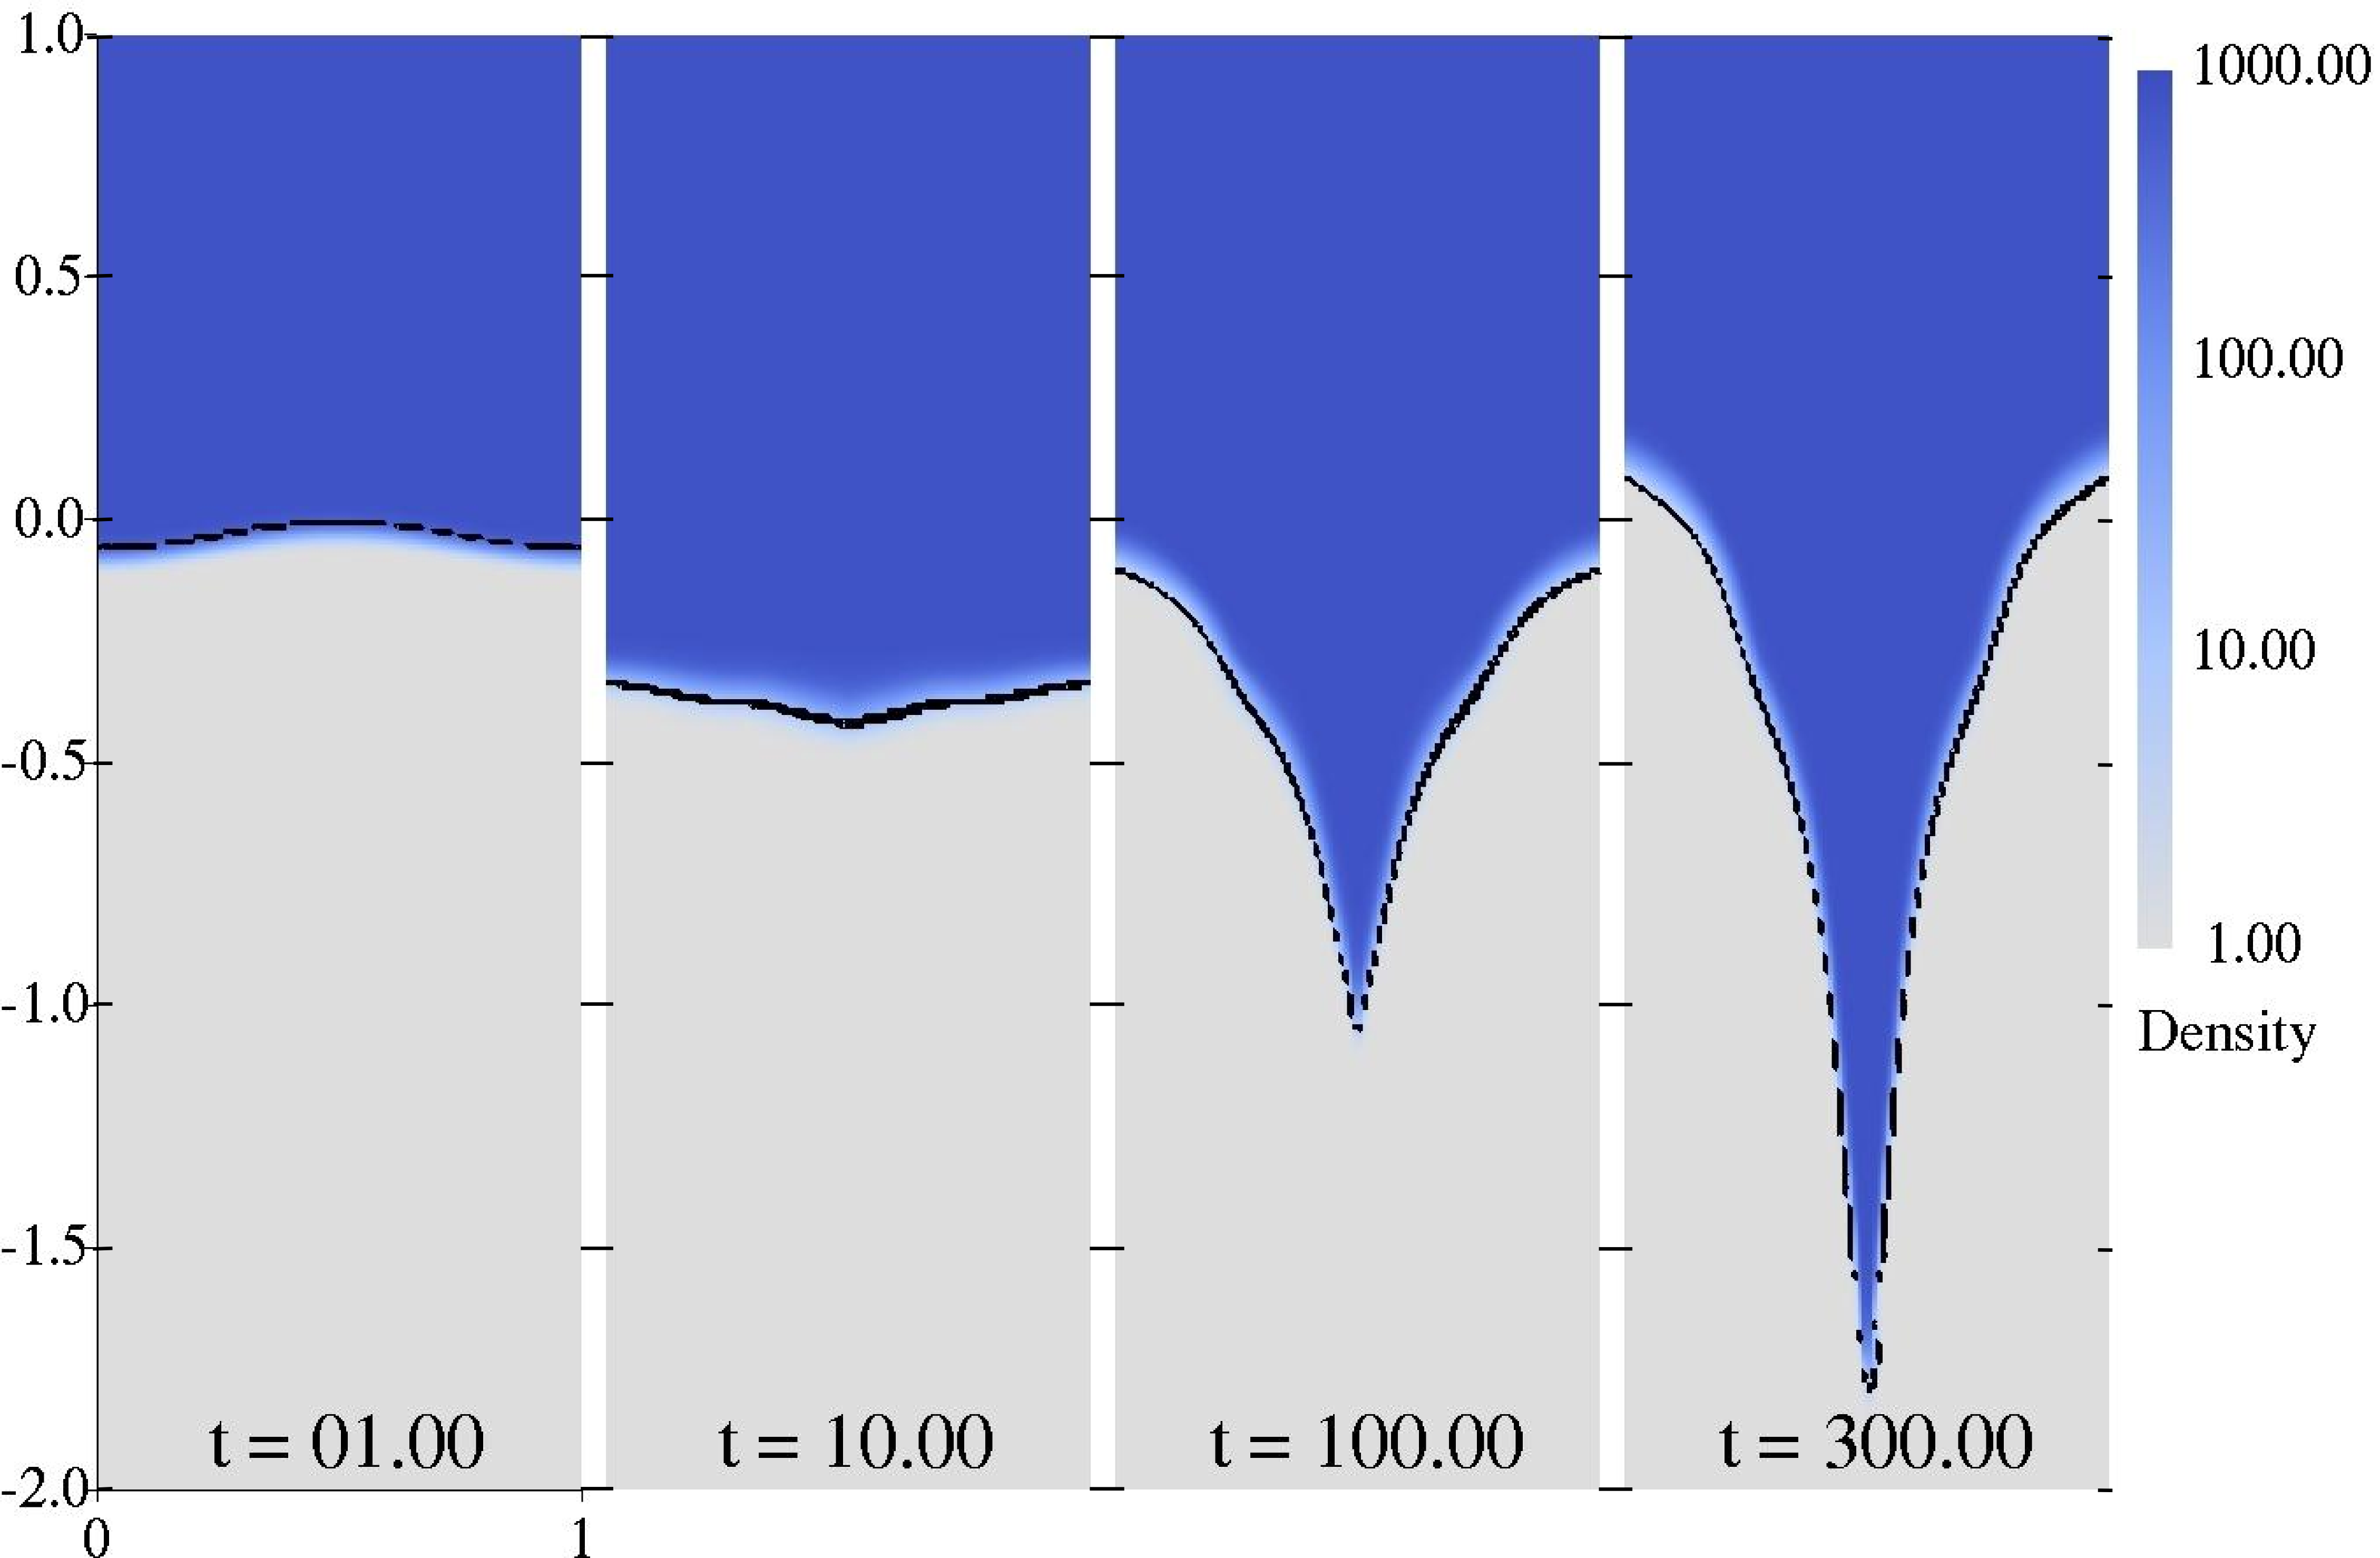
\includegraphics[width=0.9\textwidth]{./figs/lung_figs/snapshots_density_t1}
%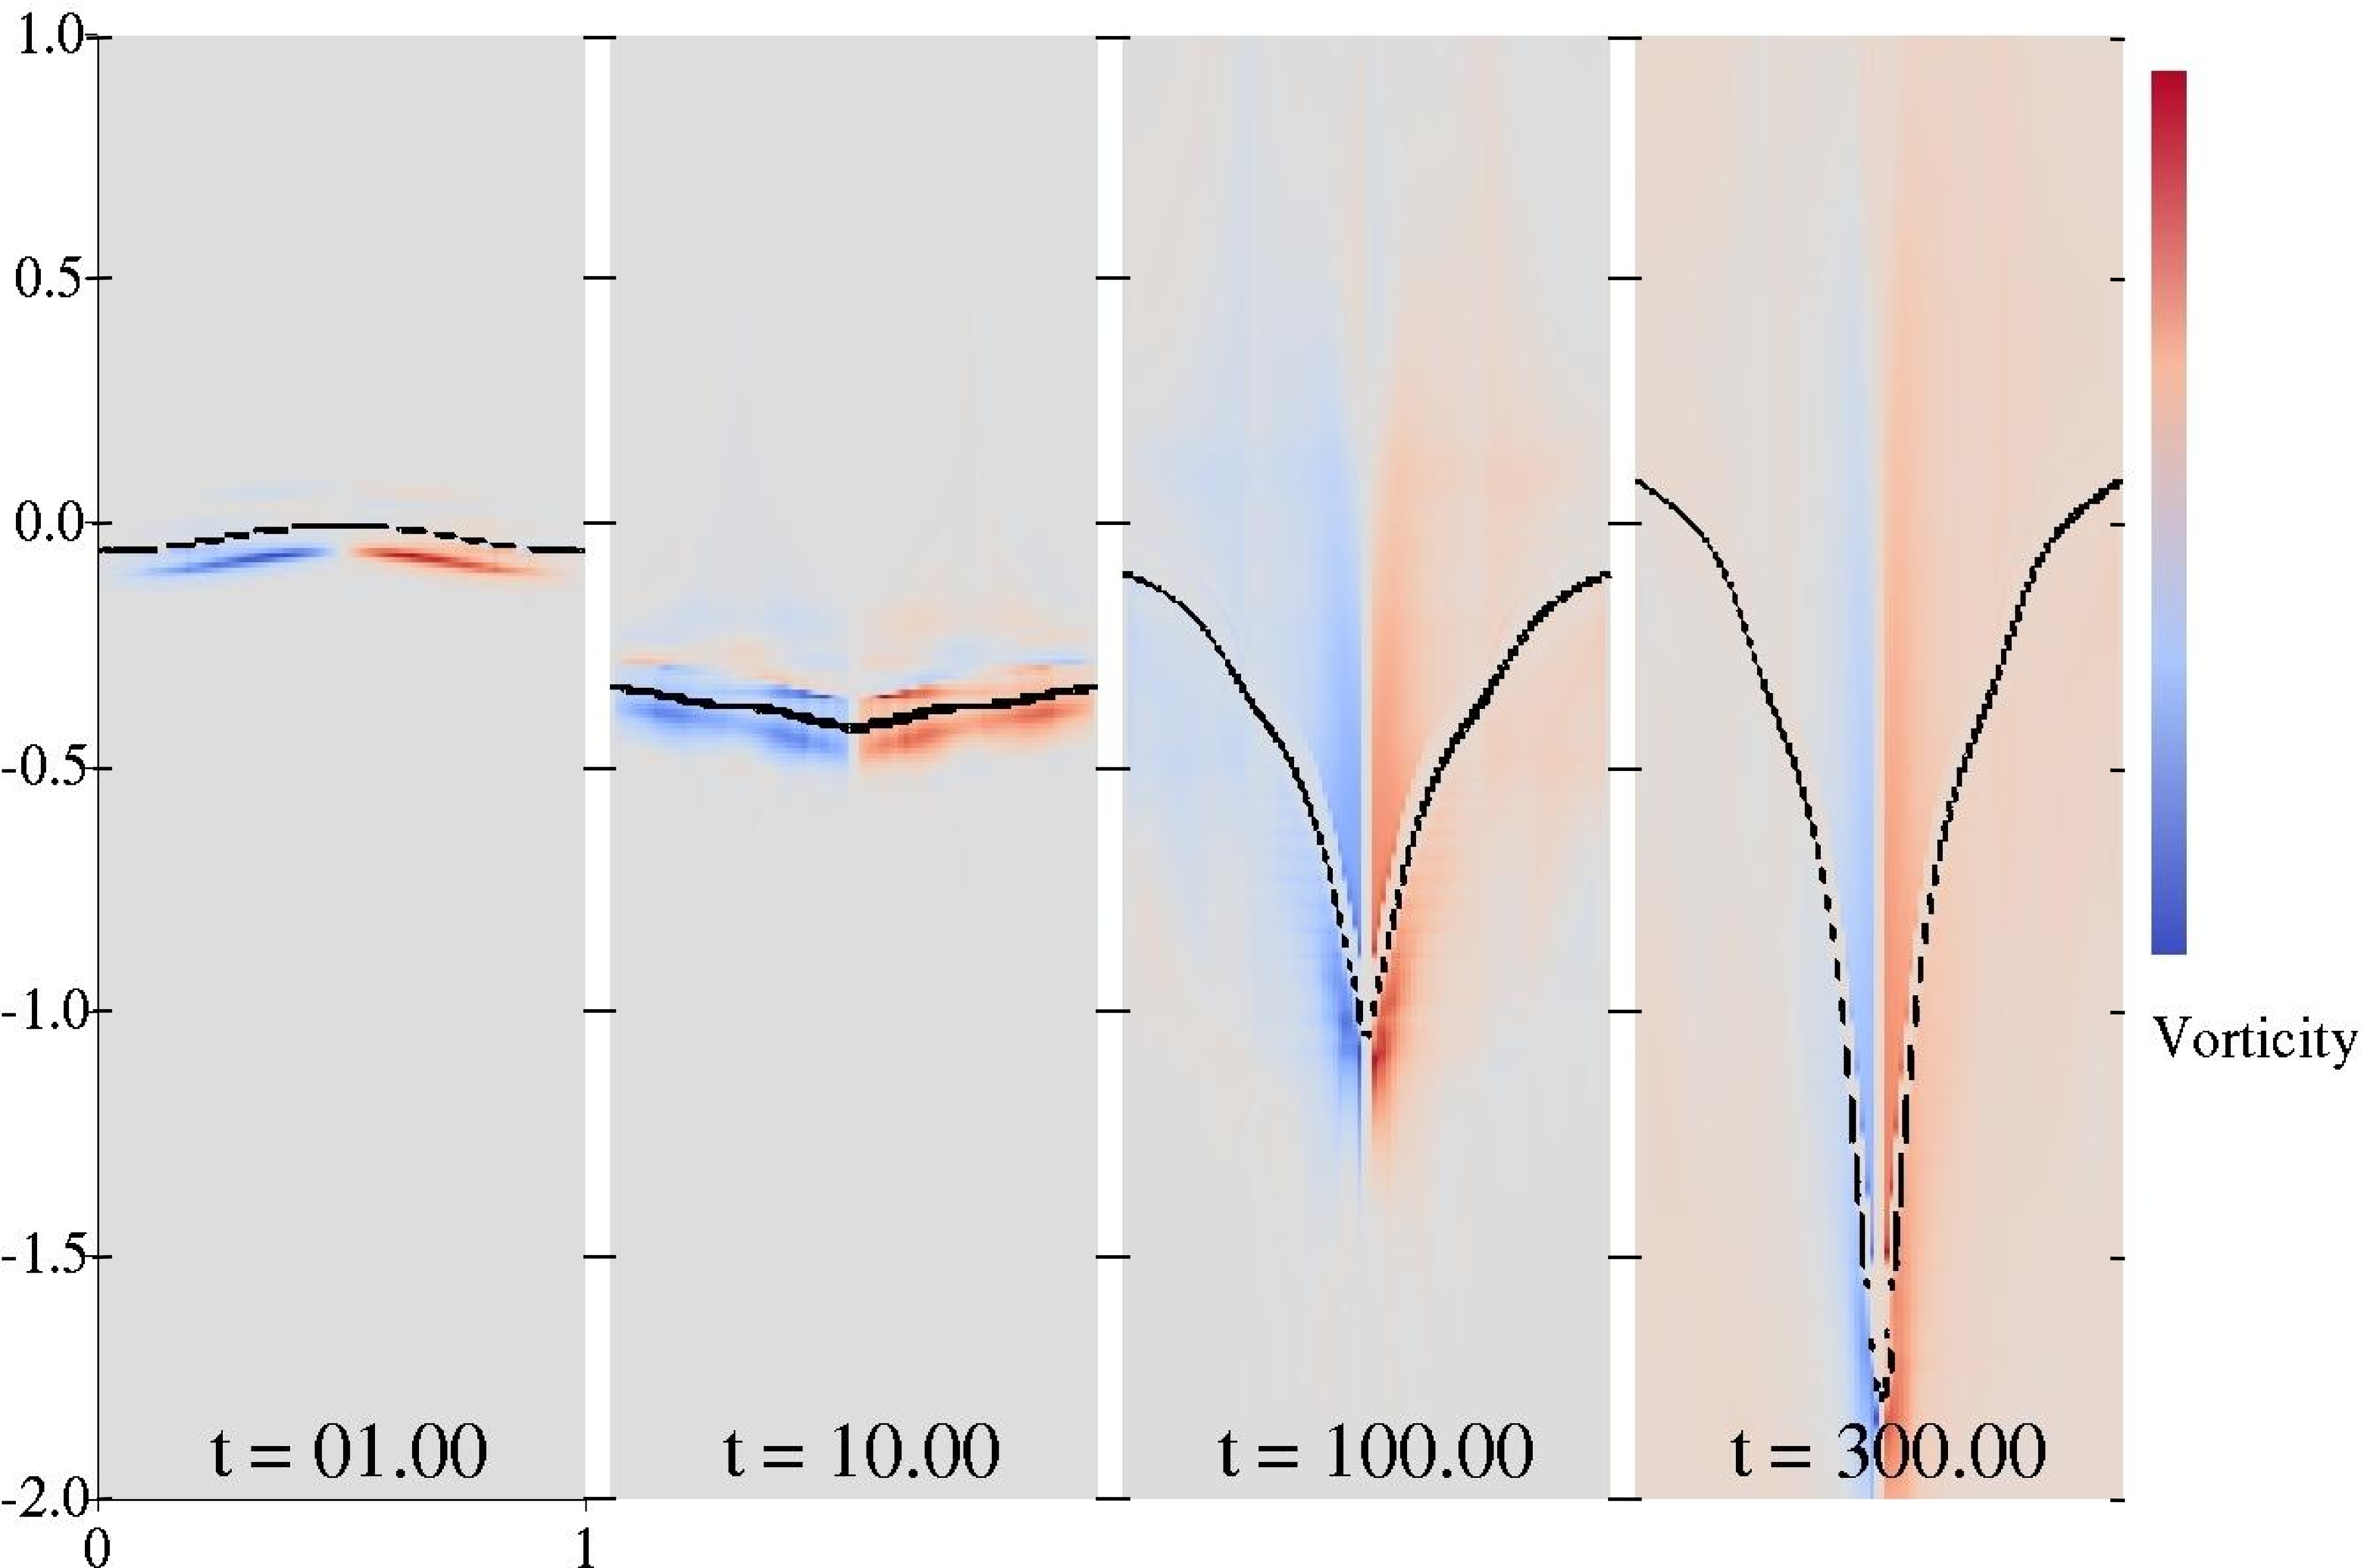
\includegraphics[width=0.9\textwidth]{./figs/lung_figs/snapshots_vorticity_t1}
\caption[The evolution of the acoustically perturbed interface]
{Surface plots of density throughout the evolution of the interface,
  at $t=1, 10, 100, 300$, for the $10$ MPa trapezoidal wave
  case. Areas of high density (i.e., water) are indicated in dark
  blue. Areas of low density (i.e., air) are indicated in white.}
  \label{fig:interface_snapshots}
\end{figure}
%
To illustrate the evolution of the interface, Figure
\ref{fig:interface_snapshots} contains color plots of the density
during the compression-interface interaction $(t=1)$, immediately
after the wave leaves the interface $(t=10)$, and at late times
$(t=100, 300)$. Contours of 0.5 volume fraction of water are indicated
in black on both plots. The initially smooth interface perturbation
grows from a smooth sinusoid to a sharp point at late times.


\section{OLD}
%---------------------------------------------------------------------

 vorticity (Bottom) fields at different instances in
the flow's evolution. Areas of high density (i.e., water) are dark
blue and areas of low density (i.e., air) are light-blue. On the
vorticity contours, counterclockwise (positive) vorticity is red, and
clockwise (negative) vorticity is blue. The purpose of the vorticity
plots is only to show the location and direction of vorticity at each
time. For sake of visualization, the range of the vorticity color
scale changes at each time slice because the vorticity spreads over
time. Hence the vorticity magnitudes are not shown here.  

The initially smooth interface perturbation grows from a smooth
sinusoid to a sharp spike at late time.  vorticity is heavily
concentrated in the air. At $t=1$, the compression-interface
interaction has nearly completed and 97\% of the total circulation in
the left or right half domain exists in fluid with volume fraction
$\alpha<0.5$. This is qualitatively consistent with our analysis. As
time progresses, it can be seen that the vorticity disperses
throughout the domain, but remains concentrated around the interface
and the vertical center of the domain.

To more closely exam the interface and circulation dynamics associated
with the compression wave-interface interaction, Figure
\ref{fig:trapz10_circ_interface} shows the early-time histories of the
interface amplitude $a(t)$ and half-domain circulation $\Gamma$. We
have labeled the times at which different portions of the incoming
wave encounter the interface as $t_{1-4}$, denoted with black
$\bs{\times}$s along the curves in these figures and those
hereafter. From $t_1=0^+$ to $t_2$ the compression wave encounters the
interface. During this interaction the perturbation amplitude
decreases, and the right half-domain circulation $\Gamma$ rises
sharply. At $t_2\approx1.1$, the pressure reaches its maximum
amplitude, $p_a=10$ MPa, and remains constant until $t_3$. We note
that at $\overline{a(t_{1-2})}/a_0\approx0.96$, suggesting that the
static interface assumption made in our vorticity generation order of
magnitude analysis was reasonable. The interface amplitude continues
to decrease and the half-domain circulation $\Gamma$ stops its rapid
growth and changes little during this static elevated pressure period,
until the expansion wave hits at $t_3$. At $t\approx 5.0$, the
perturbation undergoes a phase inversion and begins to grow, as is
observed for the heavy-light interface Richtmyer-Meshkov problem. At
$t_3\approx8.5$ the expansion wave first hits the interface. The
perturbation amplitude continues to grow, and $\Gamma$ increases
sharply again. At $t_4\approx9.7$ the acoustic wave has finished
traversing the interface, and atmospheric pressure is resumed. The
perturbation amplitude $a_0$ continues to grow long after the
wave-interface interaction has finished.
%
\begin{figure}[h] 
  \centering
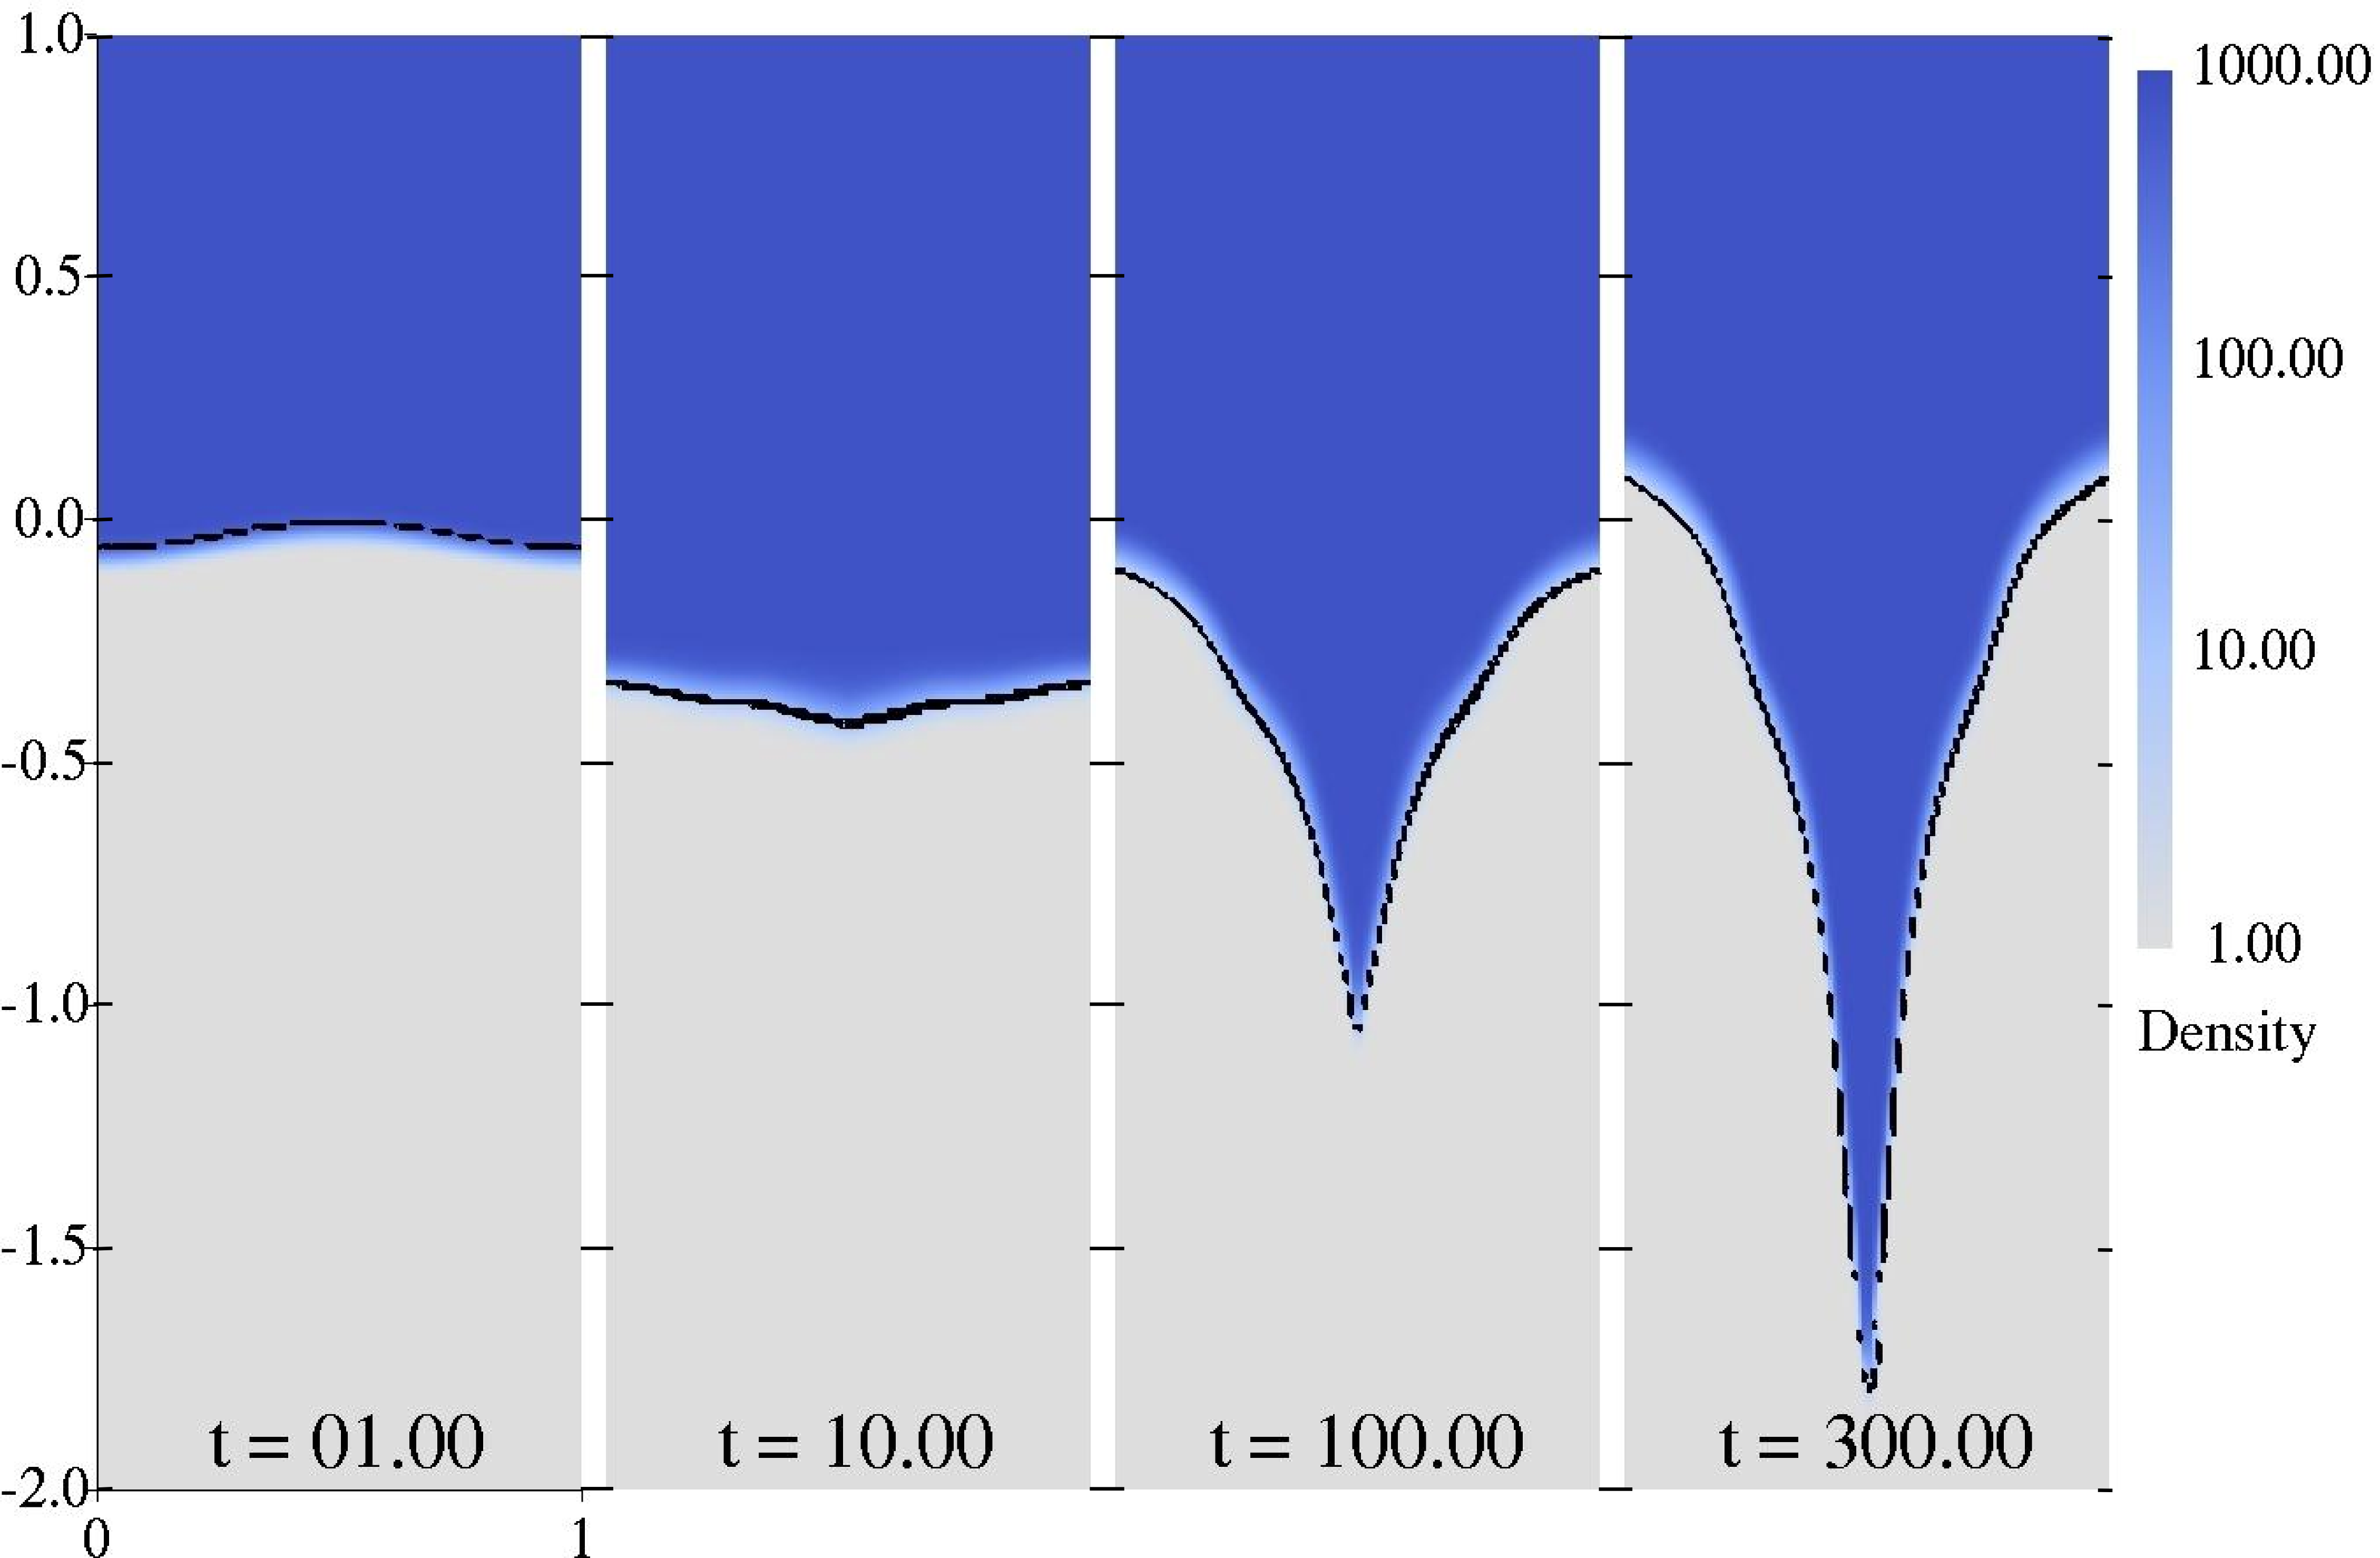
\includegraphics[width=0.9\textwidth]{./figs/lung_figs/snapshots_density_t1}
%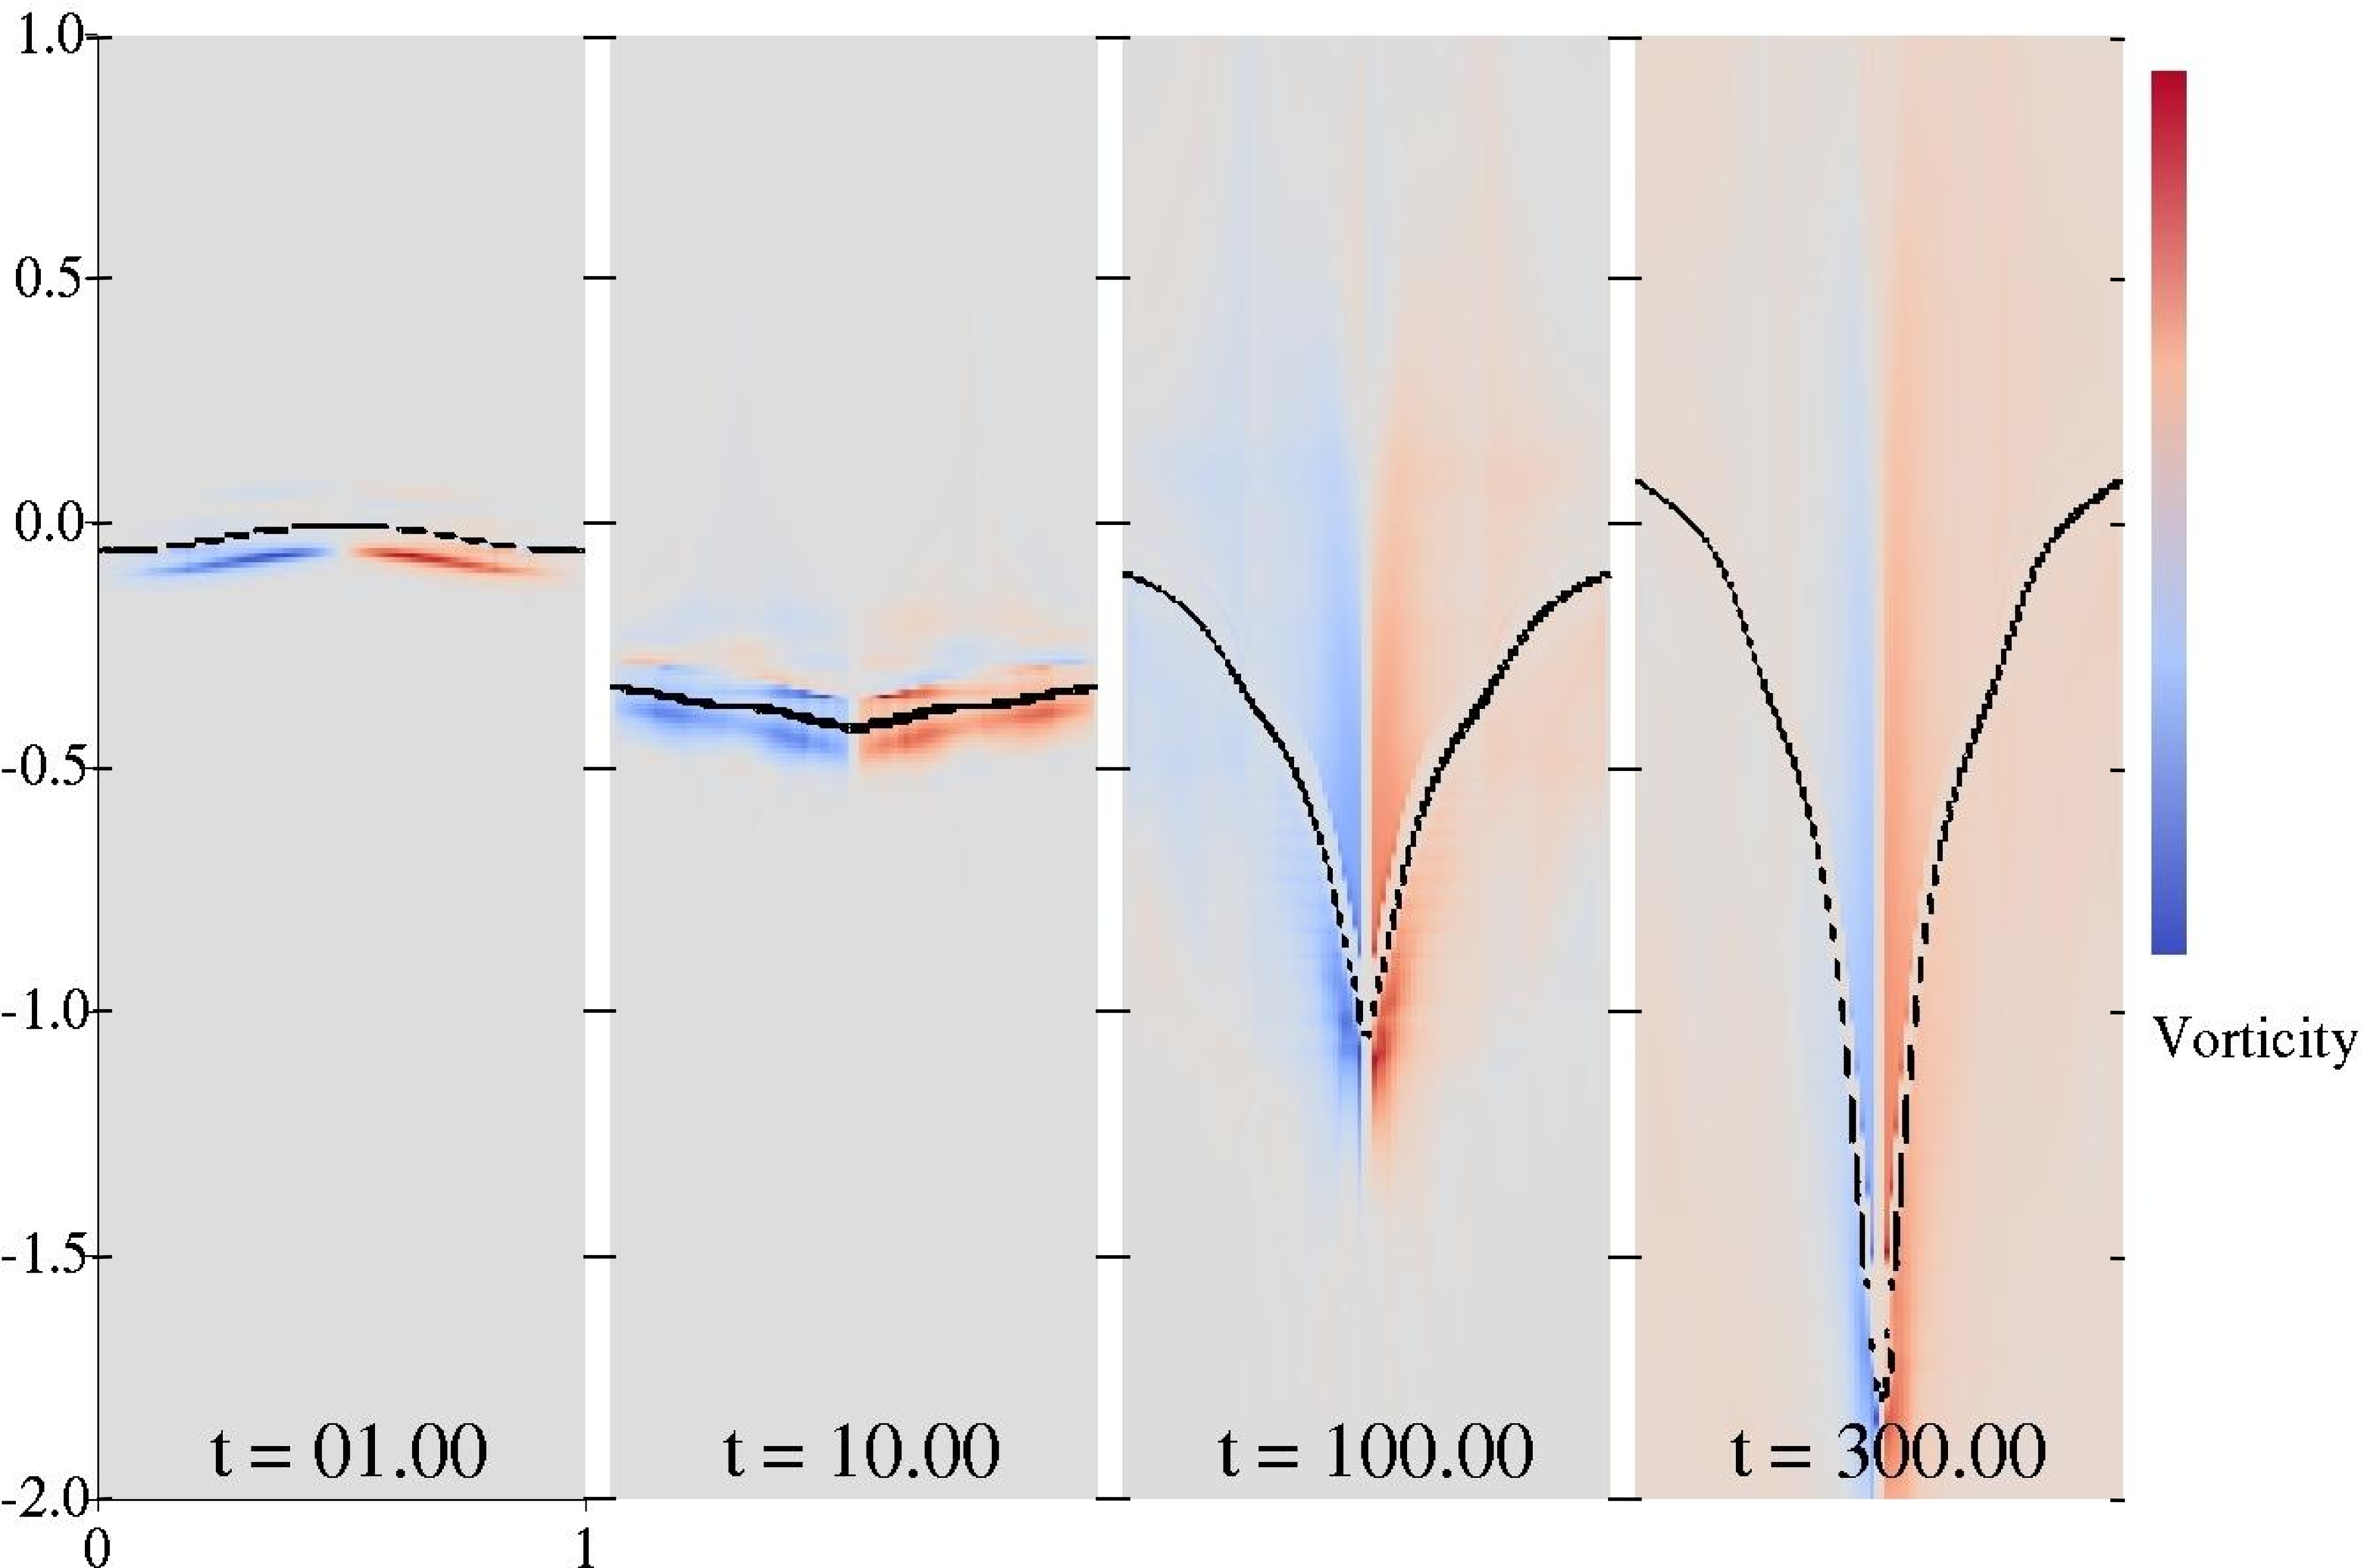
\includegraphics[width=0.9\textwidth]{./figs/lung_figs/snapshots_vorticity_t1}
\caption[The evolution of the acoustically perturbed interface and vorticity field]{Surface plots of density (Top) and vorticity (Bottom)
  throughout the evolution of the interface for the $10$ MPa
  trapezoidal wave case. Areas of high density (i.e., water) are
indicated in dark blue. Areas of low density (i.e., air) are indicated
in white.  Positive (counterclockwise) vorticity is indicated in red,
and negative (clockwise) vorticity can be seen in blue.}
  \label{fig:interface_snapshots}
\end{figure}
%
\begin{figure}[h] 
  \centering
  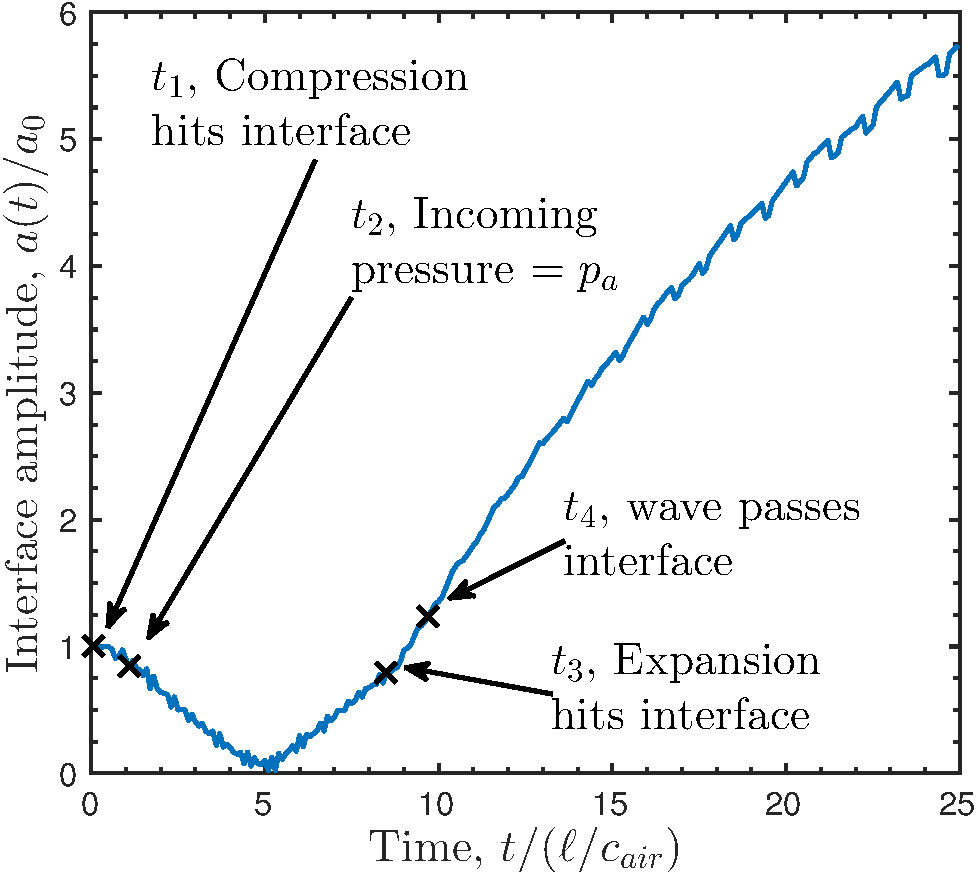
\includegraphics[width=0.48\textwidth]{./figs/lung_figs/trapz10_intf_schematic}
  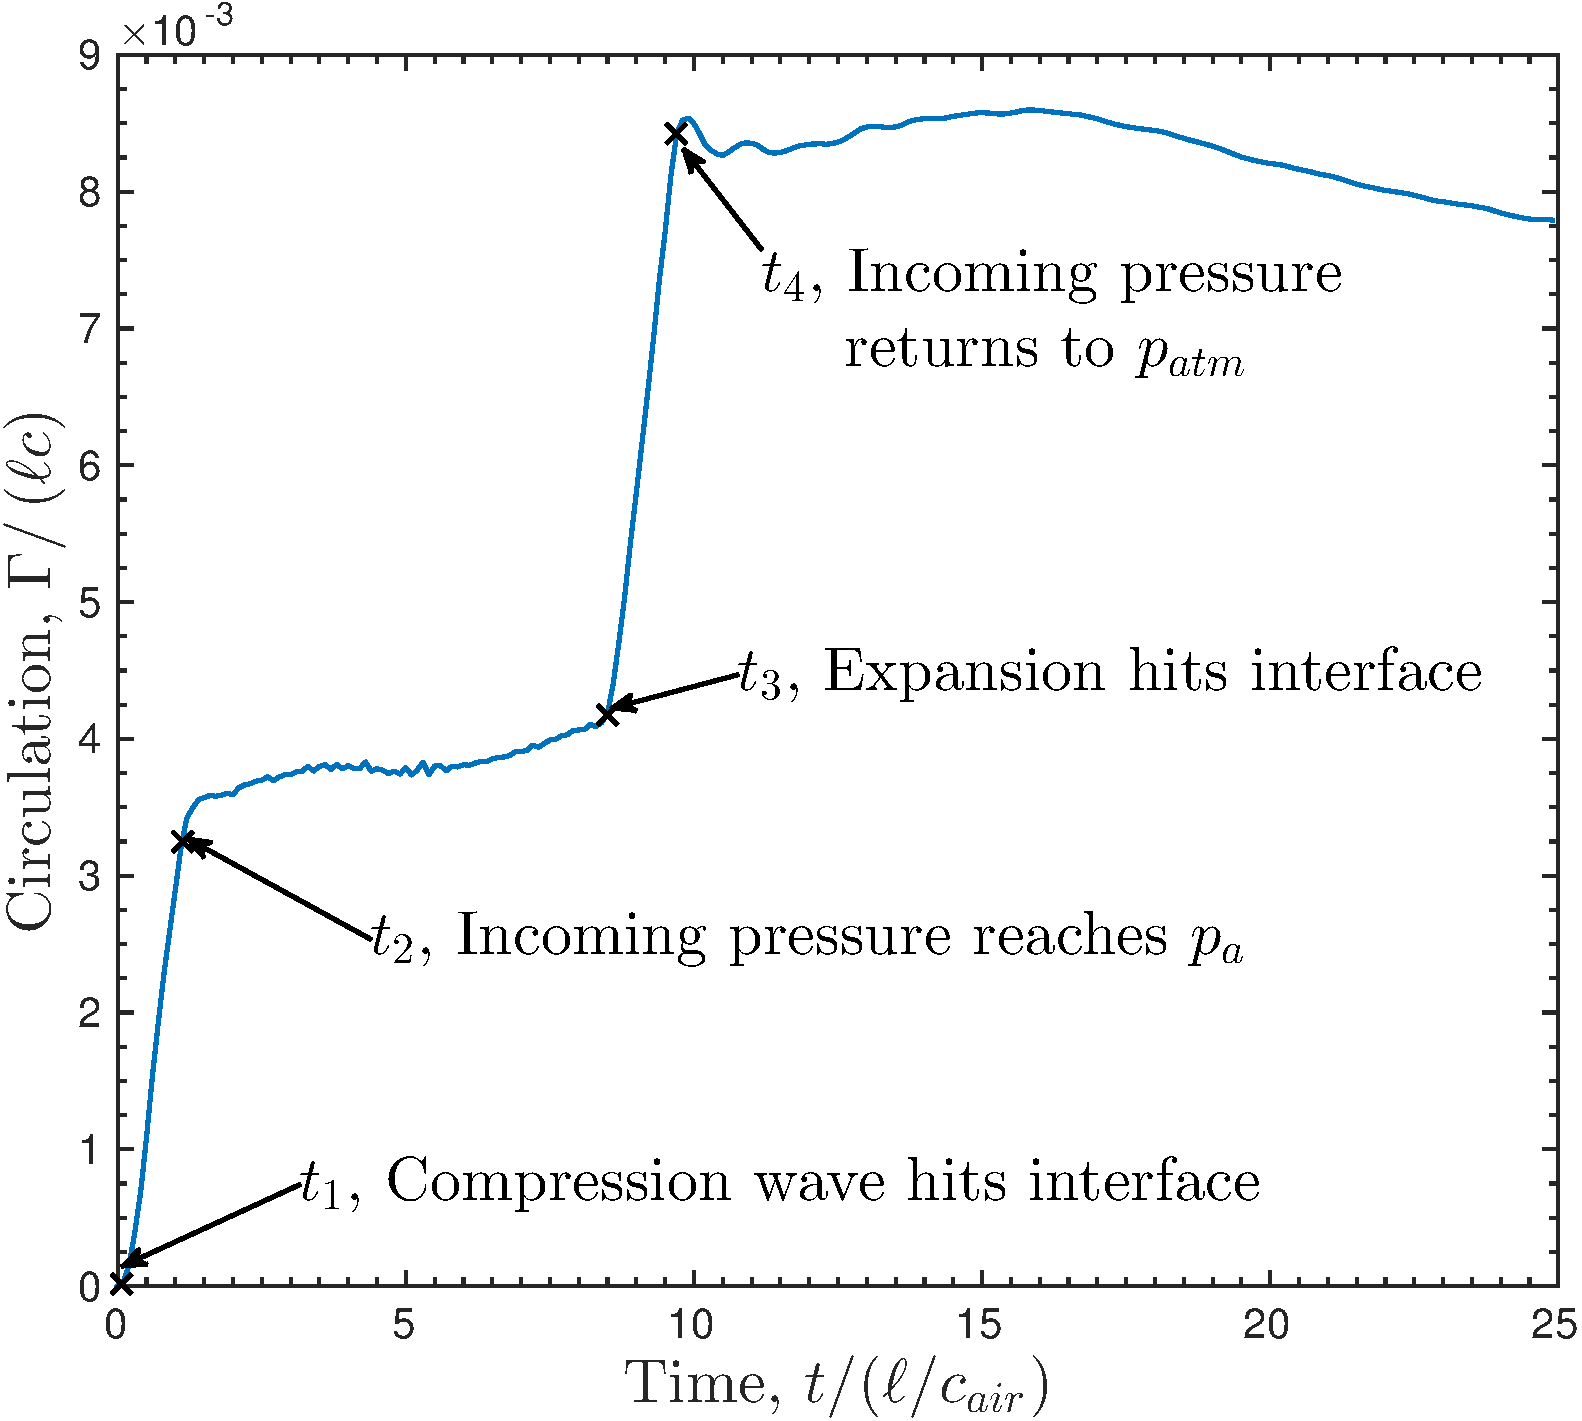
\includegraphics[width=0.48\textwidth]{./figs/lung_figs/trapz10_circ_schematic}
  \caption[The interface amplitude and circulation histories for the $10$ MPa trapezoidal wave]{The interface amplitude (left) and circulation (right)
    histories corresponding to the $10$ MPa trapezoidal waves are
    shown for $t\leq25$. Indicated times, $t_{1-4}$, are the times at
    which different stages of the incoming trapezoidal pressure wave
    shown in Figure \ref{fig:p0} first encounter the interface.}
  \label{fig:trapz10_circ_interface}
\end{figure}
%
%
\subsubsection{Dependence on acoustic wave amplitude}%
\label{subsubsec:amplitude_dependence}%
To investigate the dependence of the dynamics on the trapezoidal wave
amplitude, we compare results for $p_a=1$, $5$, and $10$ MPa while
keeping the initial lengths of the wave $L$ and the rise and fall
$\Delta L_a$ constant such that $p_a$ scales linearly with the
acoustic pressure gradient. Figure
\ref{fig:trapz_circ_interface_early}, illustrates the interface
amplitude and $p_a$-normalized circulation histories for $t\leq25$,
during and shortly after the wave-interface interaction. Black
$\bs{\times}$s along the curves indicate $t_{1-4}$, described
previously in Subsection \label{subsec:Qualitative}. During the
interaction between the interface and the compression wave, the rate
at which the perturbation amplitude decreases is greater for higher
amplitude waves. The circulation deposited during this period scales
linearly with $p_a$ as is consistent with baroclinically-generated
circulation based on our analysis. For the $10$ MPa wave, the phase of
the interface inverts at, before the expansion hits, causing
circulation deposited by the expansion to have the same sign as that
deposited by the compression. For the $1$ and $5$ MPa waves interface
phase inversion occurs after the expansion and consequently deposits
circulation opposite that of the compression wave.

Figure \ref{fig:trapz_circ_interface_loglog} \hl{(update this figure)}
shows the interface amplitude and circulation histories for $5$ and
$10$ MPa trapezoidal wave cases for $0 \leq t\leq 1000$. The
perturbation amplitude history is plotted on logarithmically-scaled
axes. For both waves, the slope of the perturbation amplitude is
approximately $0.60$ long after the waves have left the
interface. This is slightly higher than the 0.5 slope predicted by
scaling law \eqref{eq:intf_circ_scaling}. The results for the $1$ MPa
trapezoidal wave were not included because interface evolved too
slowly to obtain useful data given the computational resources available.
%
\begin{figure}[h] 
  \centering
  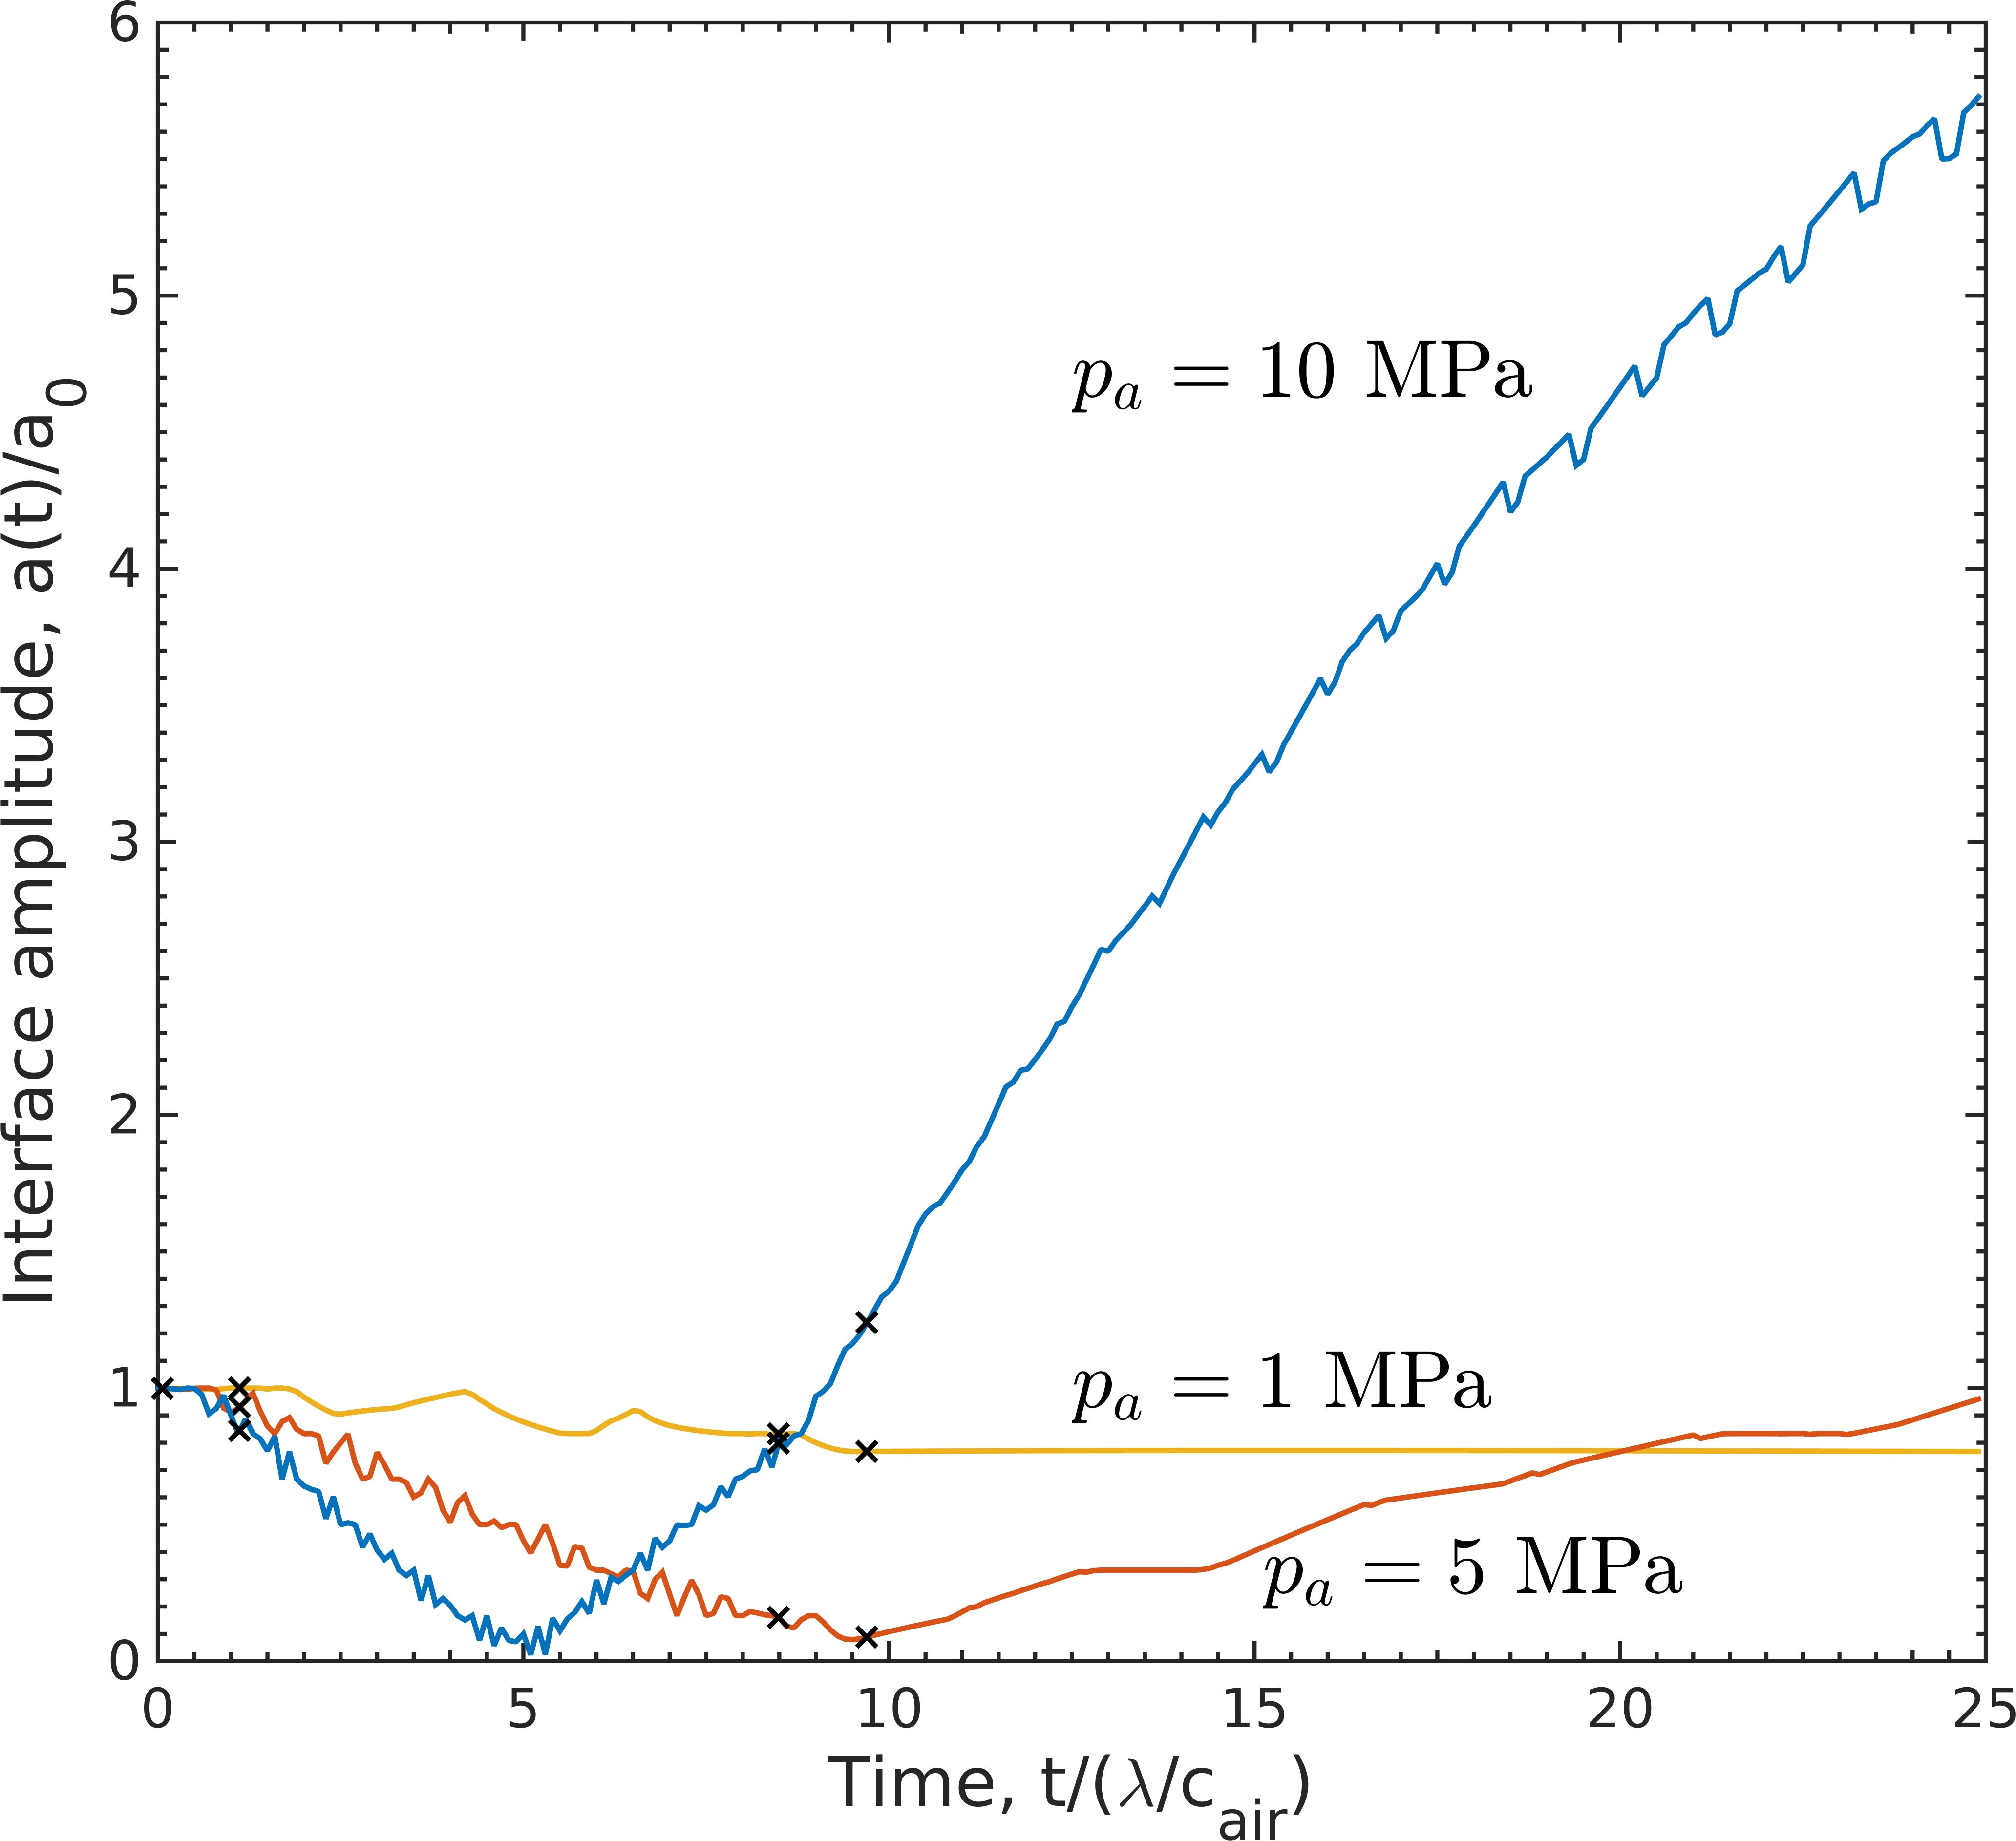
\includegraphics[width=0.48\textwidth]{./figs/lung_figs/interface_multi-amp_norm}
  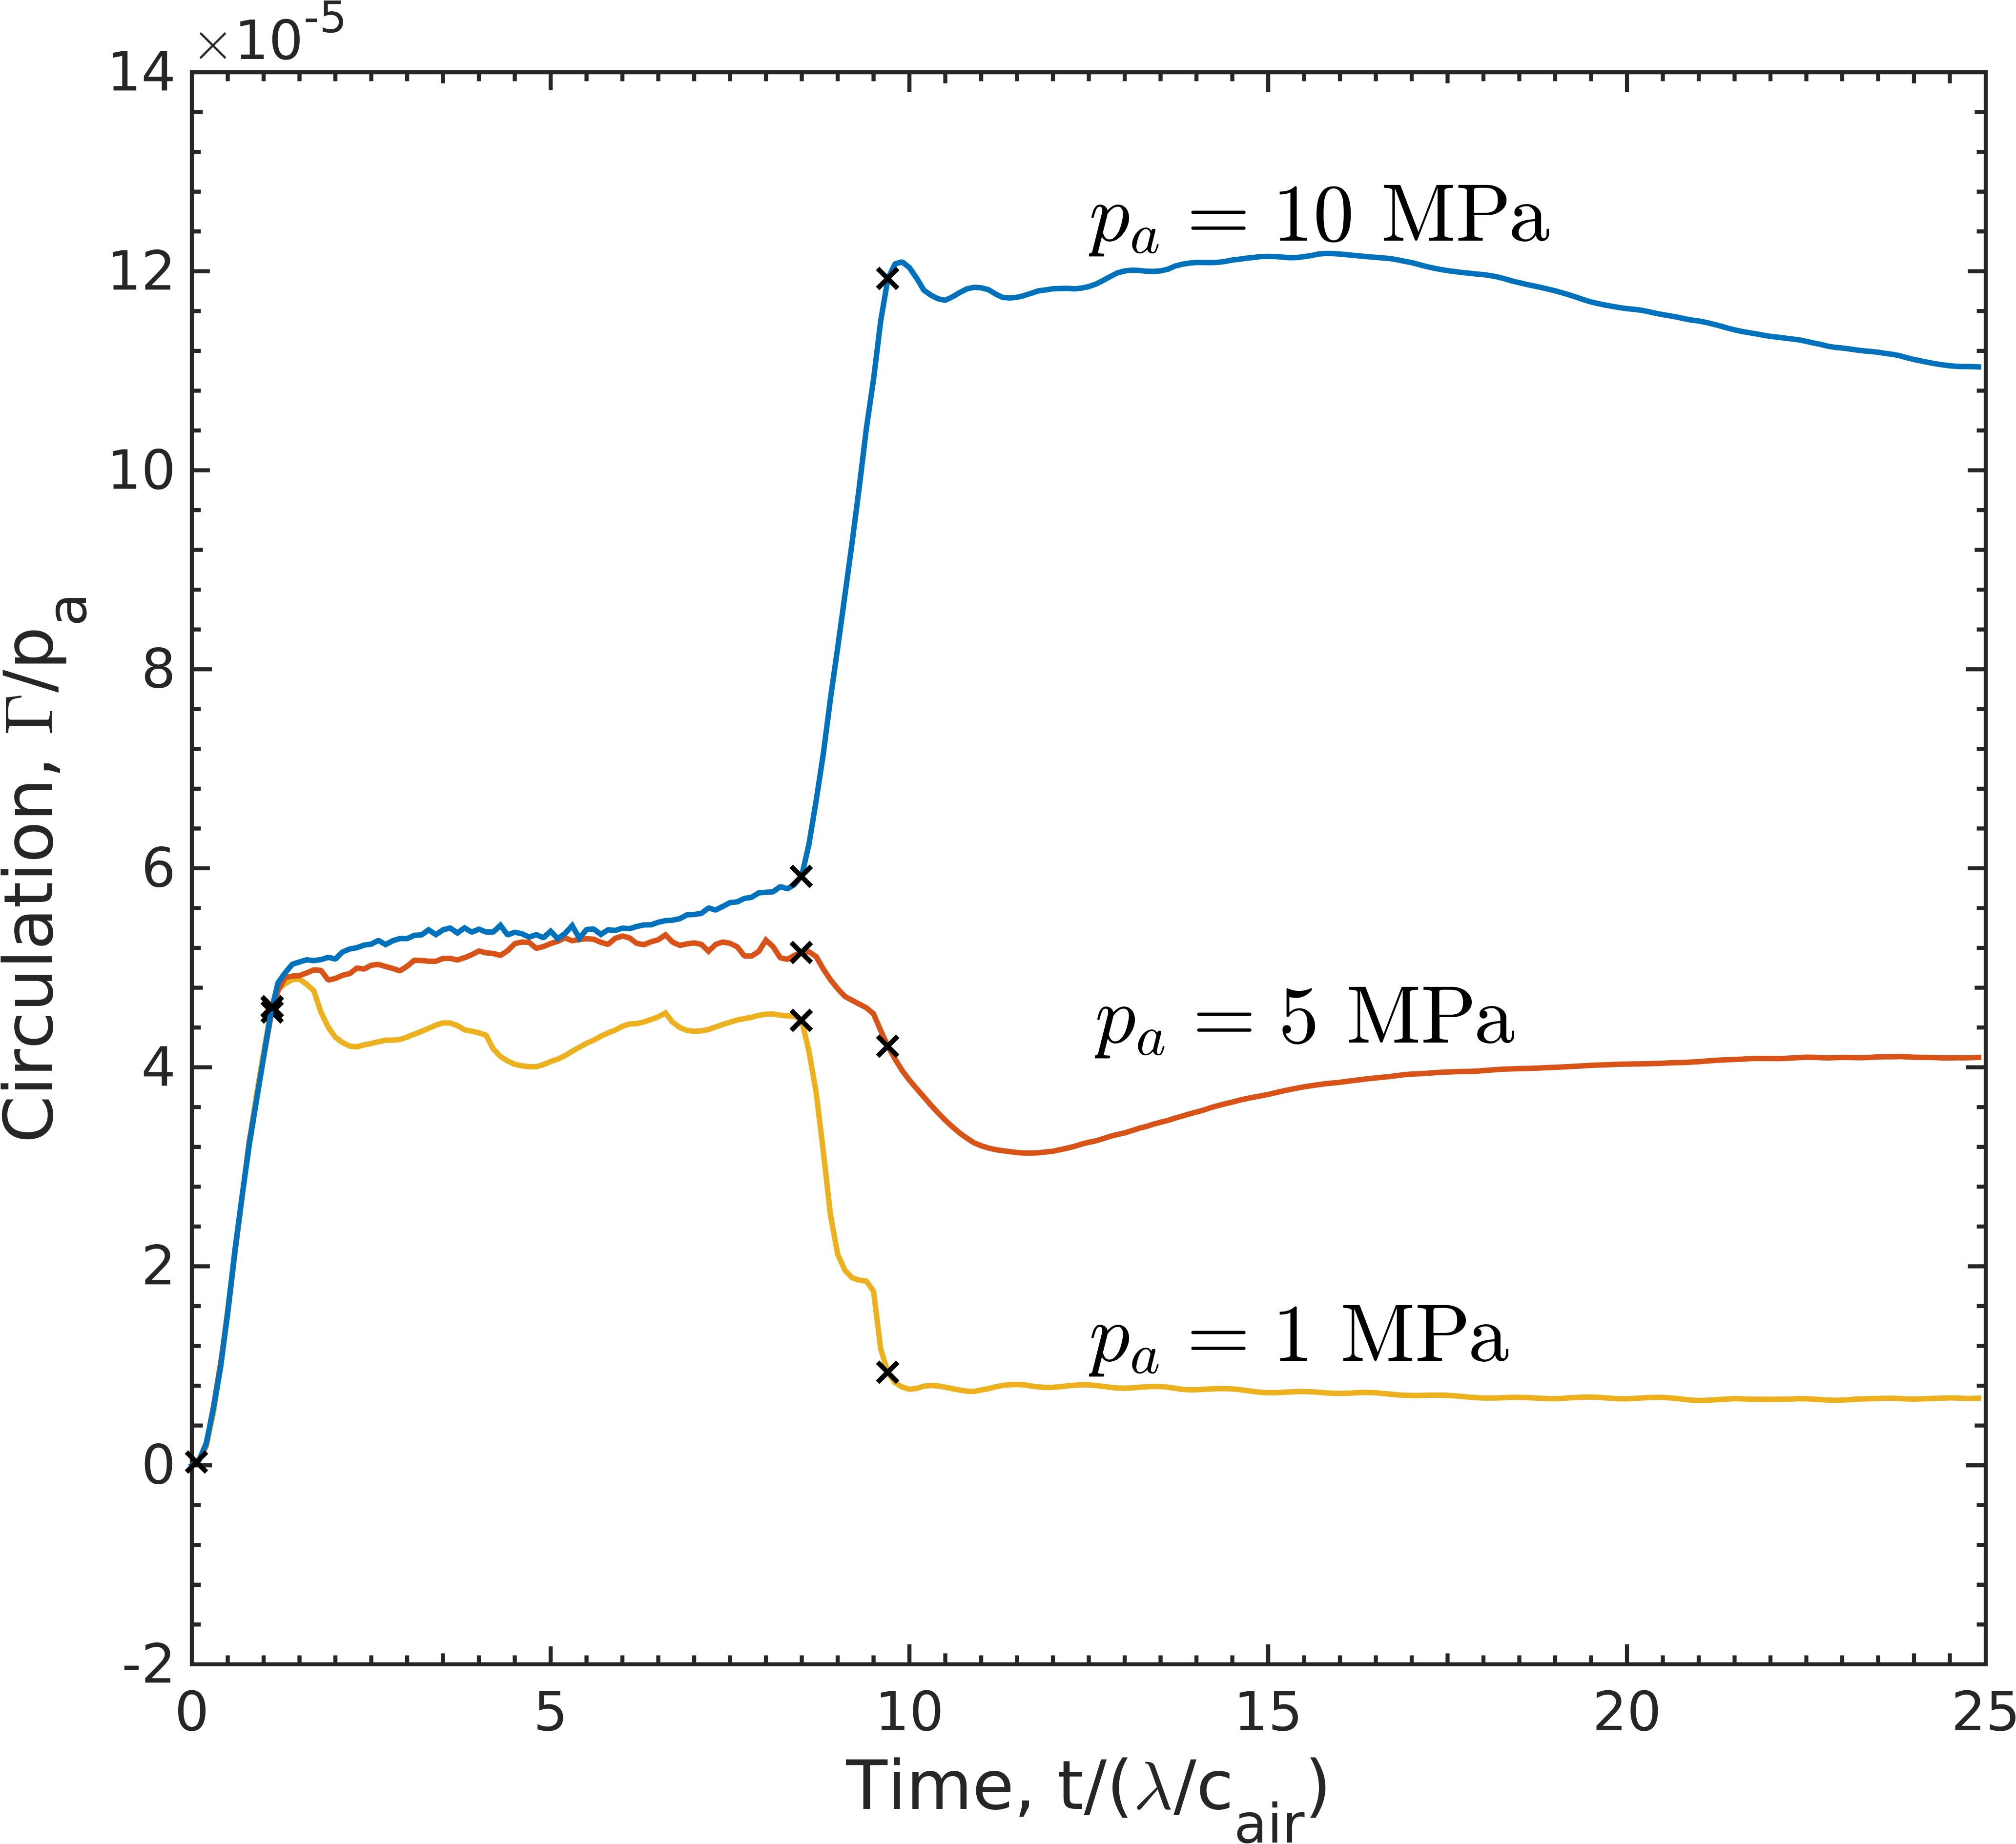
\includegraphics[width=0.48\textwidth]{./figs/lung_figs/circulation_multi-amp_norm}
  \caption[The interface and circulation dependence on wave amplitude at early time]{The interface amplitude (left) and circulation (right)
    histories corresponding to the $1$(yellow), $5$(orange), and
    $10$(blue) MPa trapezoidal waves are shown for $t\leq 25$. The
    circulation history is normalized by the acoustic amplitude of the
    incoming wave to illustrate that circulation deposition by the
    compression wave scales linearly with $p_a$.}
  \label{fig:trapz_circ_interface_early}
\end{figure}
%
\begin{figure}[h] 
  \centering
  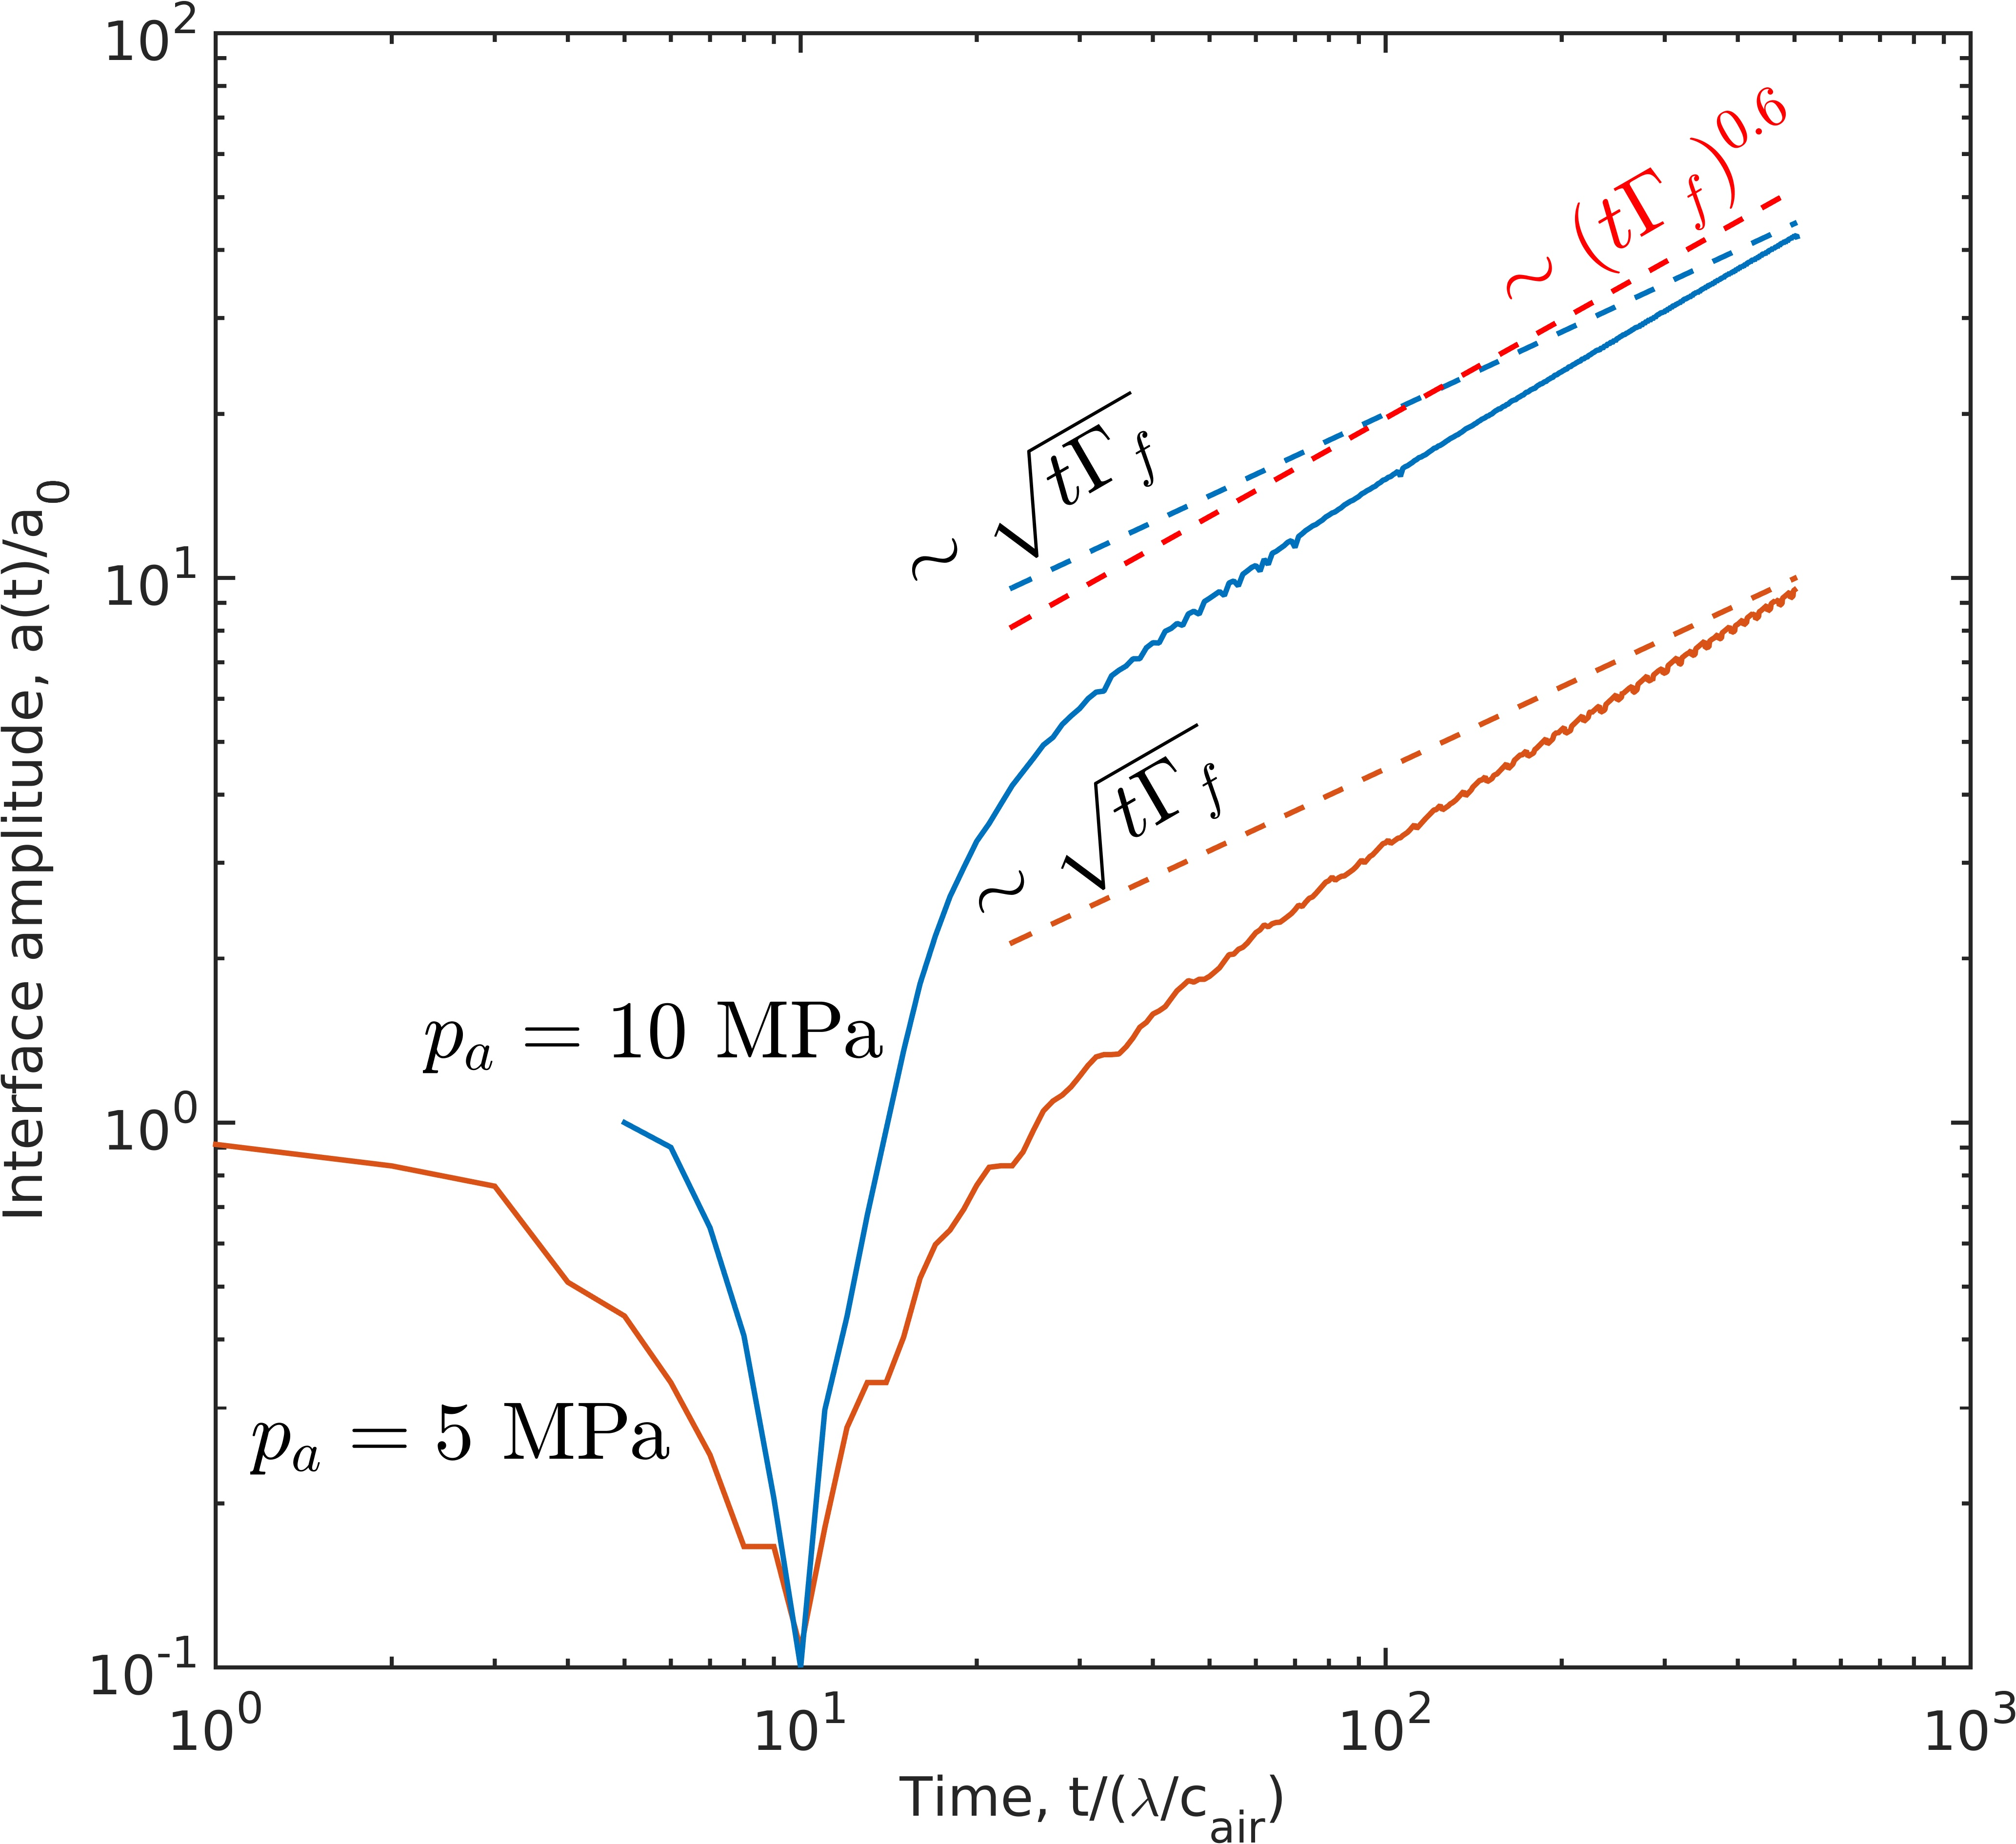
\includegraphics[width=0.48\textwidth]{./figs/lung_figs/interface_multi-amp_loglog_roe_extra}
  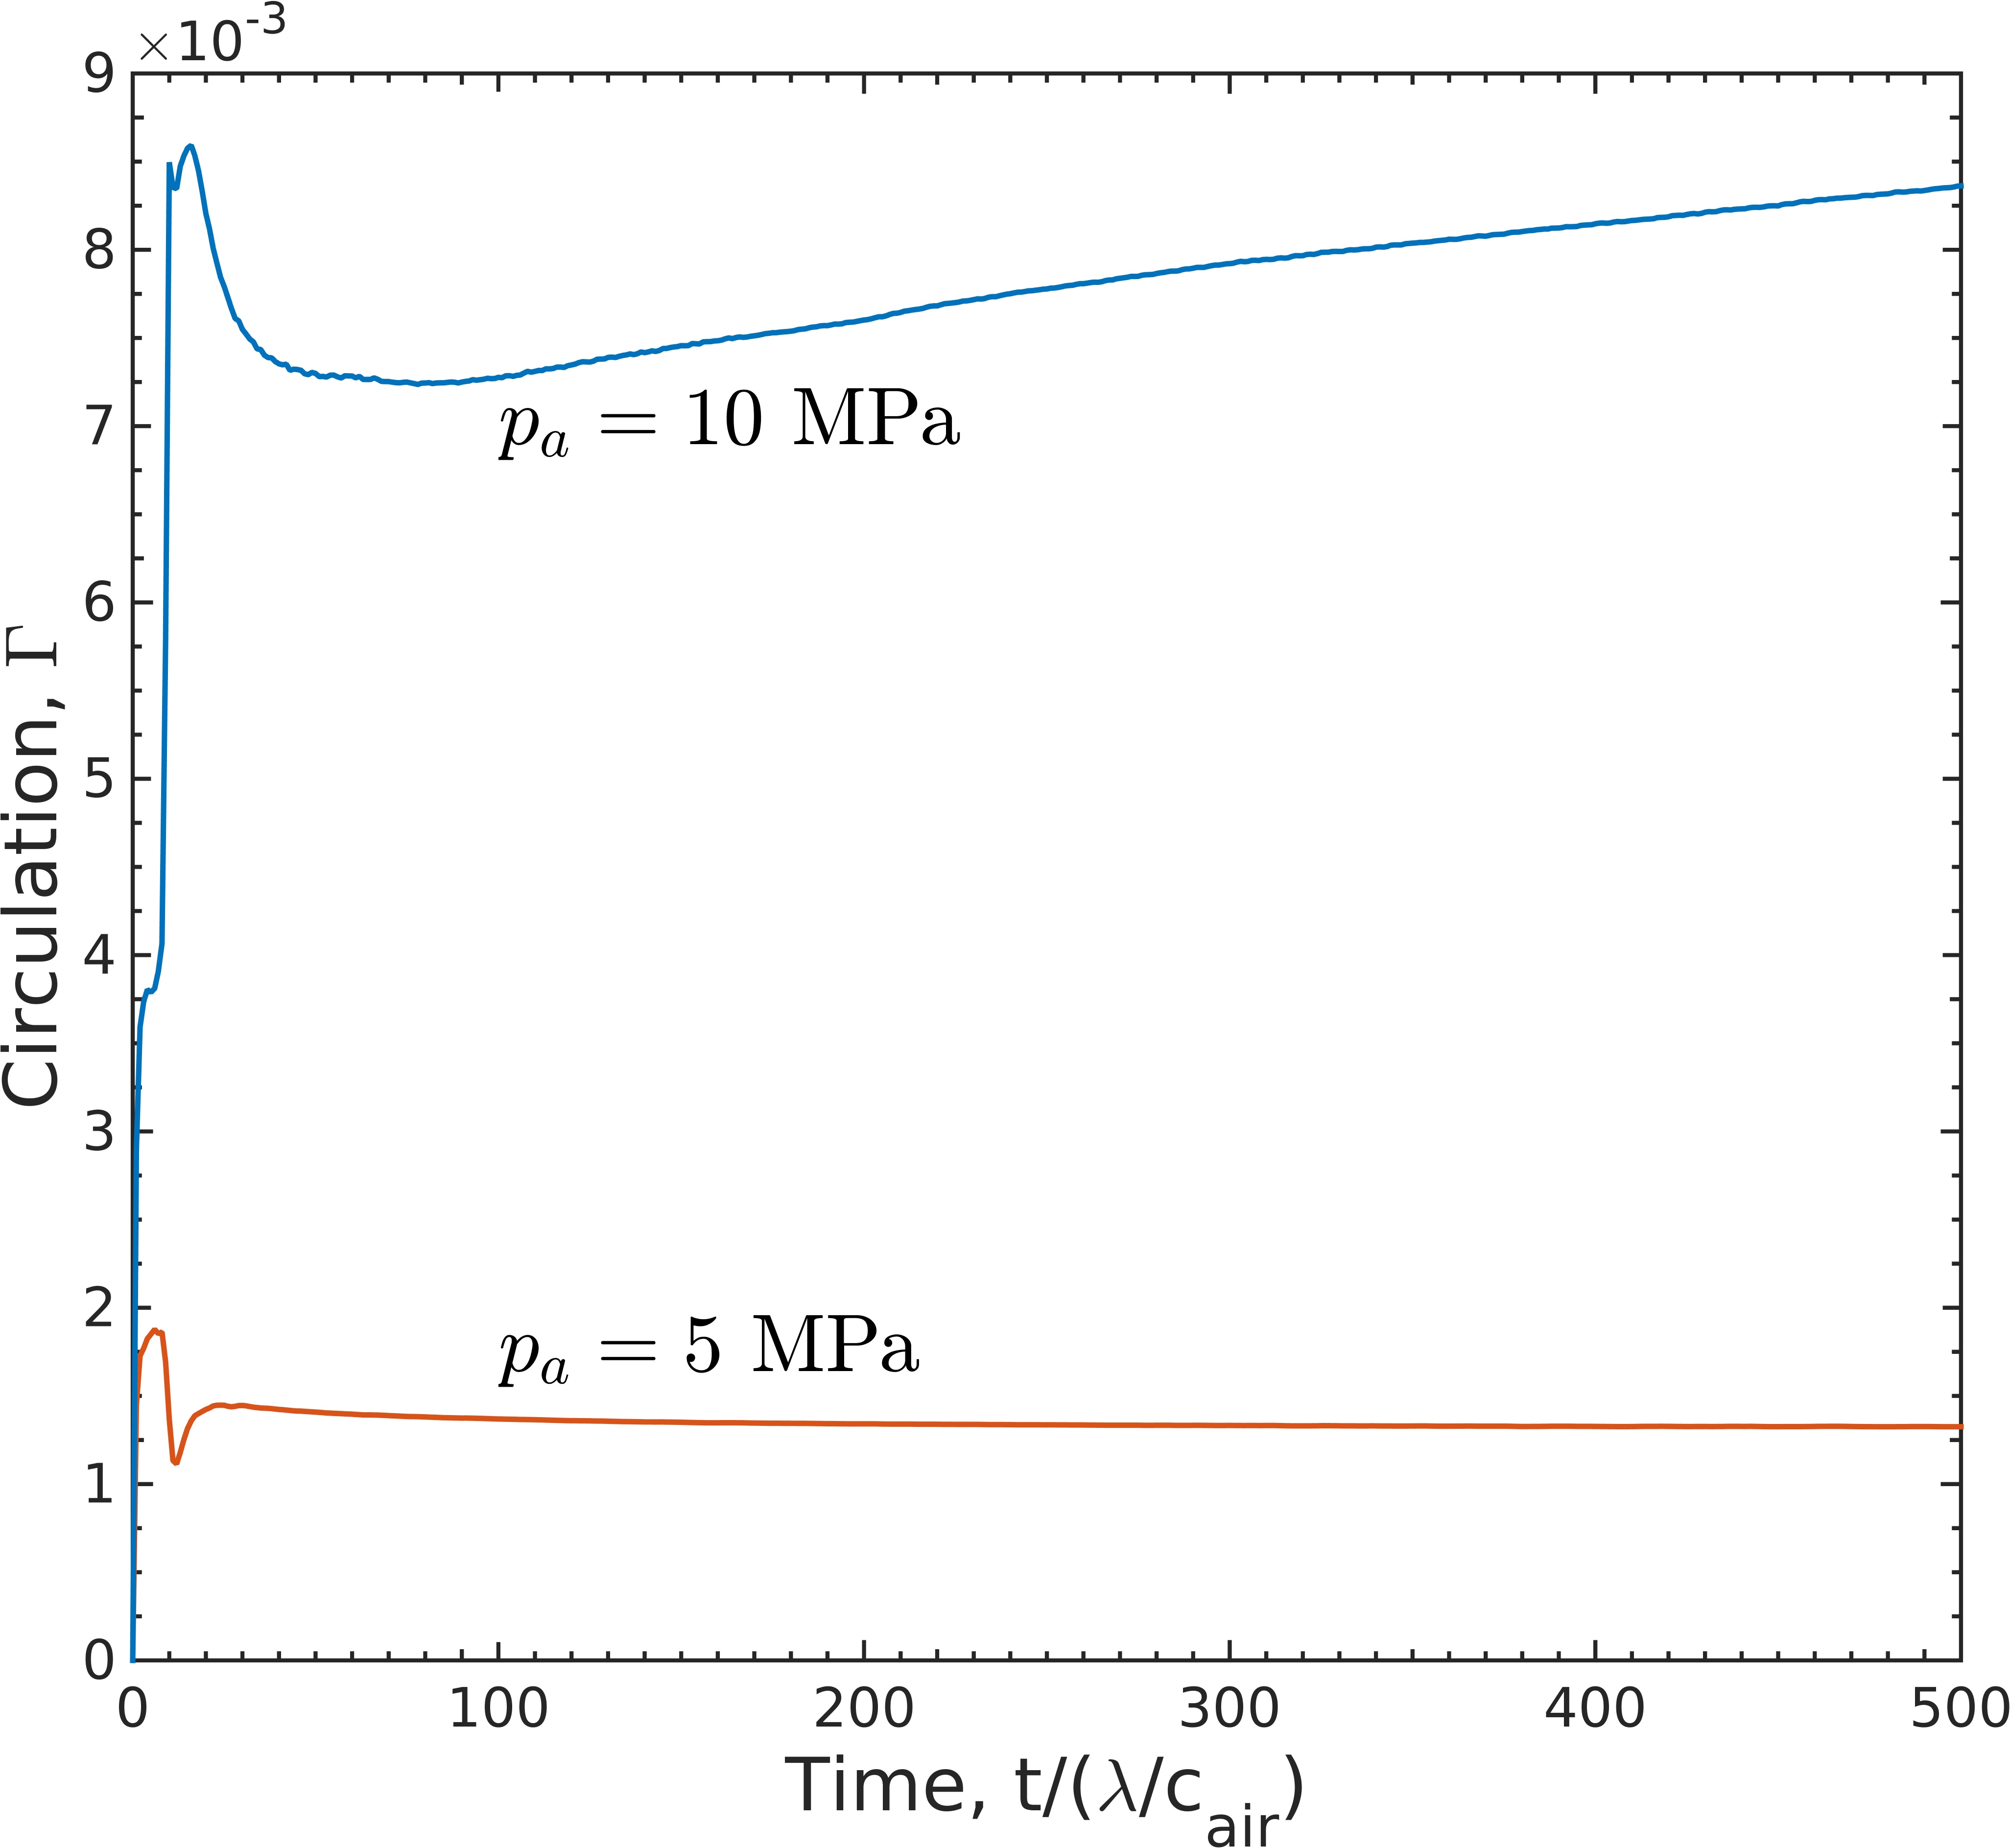
\includegraphics[width=0.48\textwidth]{./figs/lung_figs/circulation_multi-amp2_roe}
  \caption[The interface and circulation dependence on wave amplitude
  at long time]{The interface amplitude (left) and circulation (right)
    histories corresponding to the $5$(orange) and $10$(blue) MPa
    trapezoidal waves are shown for $t\leq 500$. To appropriately
    compare late time dynamics, time has been offset in the interface
    amplitude history such that the phase reversal appears to occur
    simultaneously in both simulations. Dashed lines of the same color
    are used to demonstrate the expected slope of pure circulation
    driven interface growth, based on Equation
    \eqref{eq:intf_circ_scaling}. The red dashed line shows the slope we
    appear to be approaching for the $10$ MPa wave case for the end time.}
  \label{fig:trapz_circ_interface_loglog}
\end{figure}
%
\subsubsection{Dependence on the length of the wave}%
To investigate the dependence of the dynamics on the length of the
trapezoidal wave $L$, and comparably the wave-interface interaction
time, we compare results for $p_a=10$ MPa waves of constant rise and
fall length $\Delta L_a$. This effectively changes the time the
interface has to evolve while experiencing the constant elevated
pressure portion of the wave between the compression and expansion.
Figure \ref{fig:trapz_circ_interface_multi-lag} shows the interface
amplitude and circulation histories corresponding to waves with
$L=45\lambda, 35\lambda ,30\lambda ,25\lambda ,15\lambda ,10\lambda$
for $0 \leq t\leq 25$.  For the three longest waves, $L \geq 30\lambda$,
the expansion encounters the interface after the perturbation reverses
phase. In these cases, the expansion deposits additional positive
circulation along the right half of the interface. For the shorter
waves, $L \leq 25\lambda$, the expansion encounters the interface before
the perturbation reverses phase and the net half-domain circulation is
decreased. Comparing cases in which the interface inverts phase before
the expansion occurs the larger $a(t)$ is at the time, the more
circulation is generated. The same is true when comparing cases in
which the phase inversion occurs after the interface inverts phase.
%
\begin{figure}[h] 
  \centering
  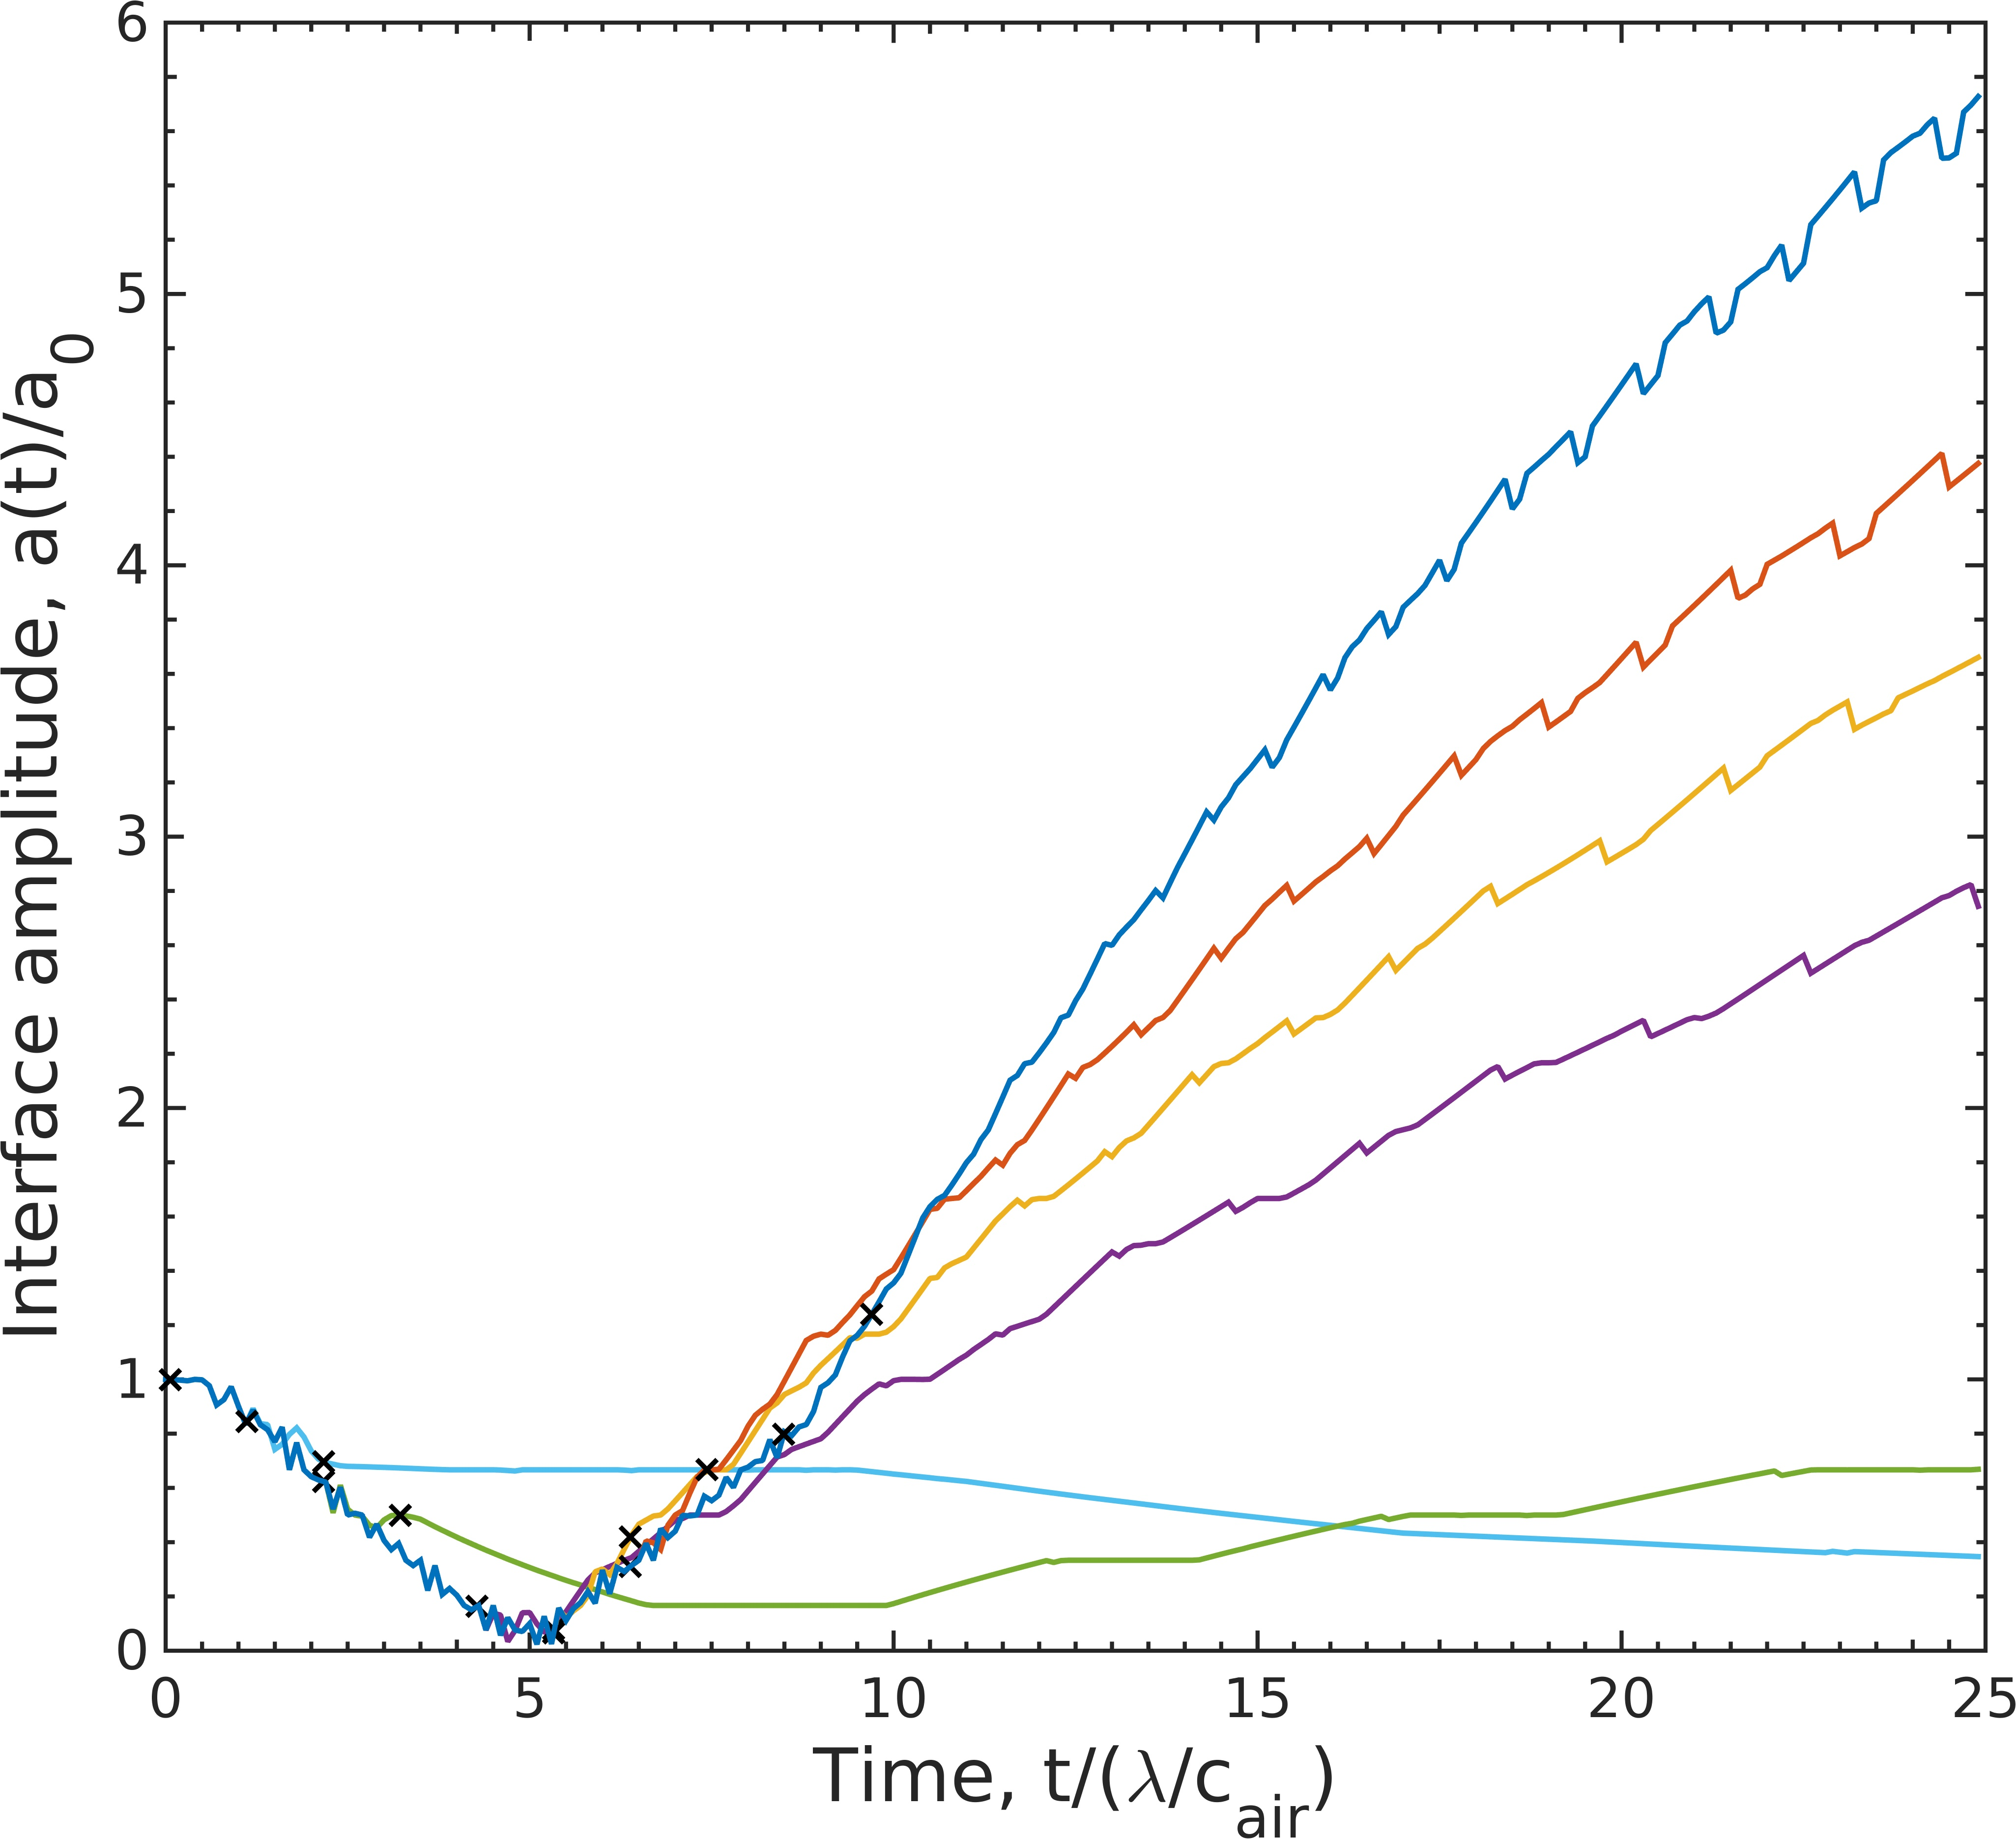
\includegraphics[width=0.48\textwidth]{./figs/lung_figs/interface_multi-lag}
  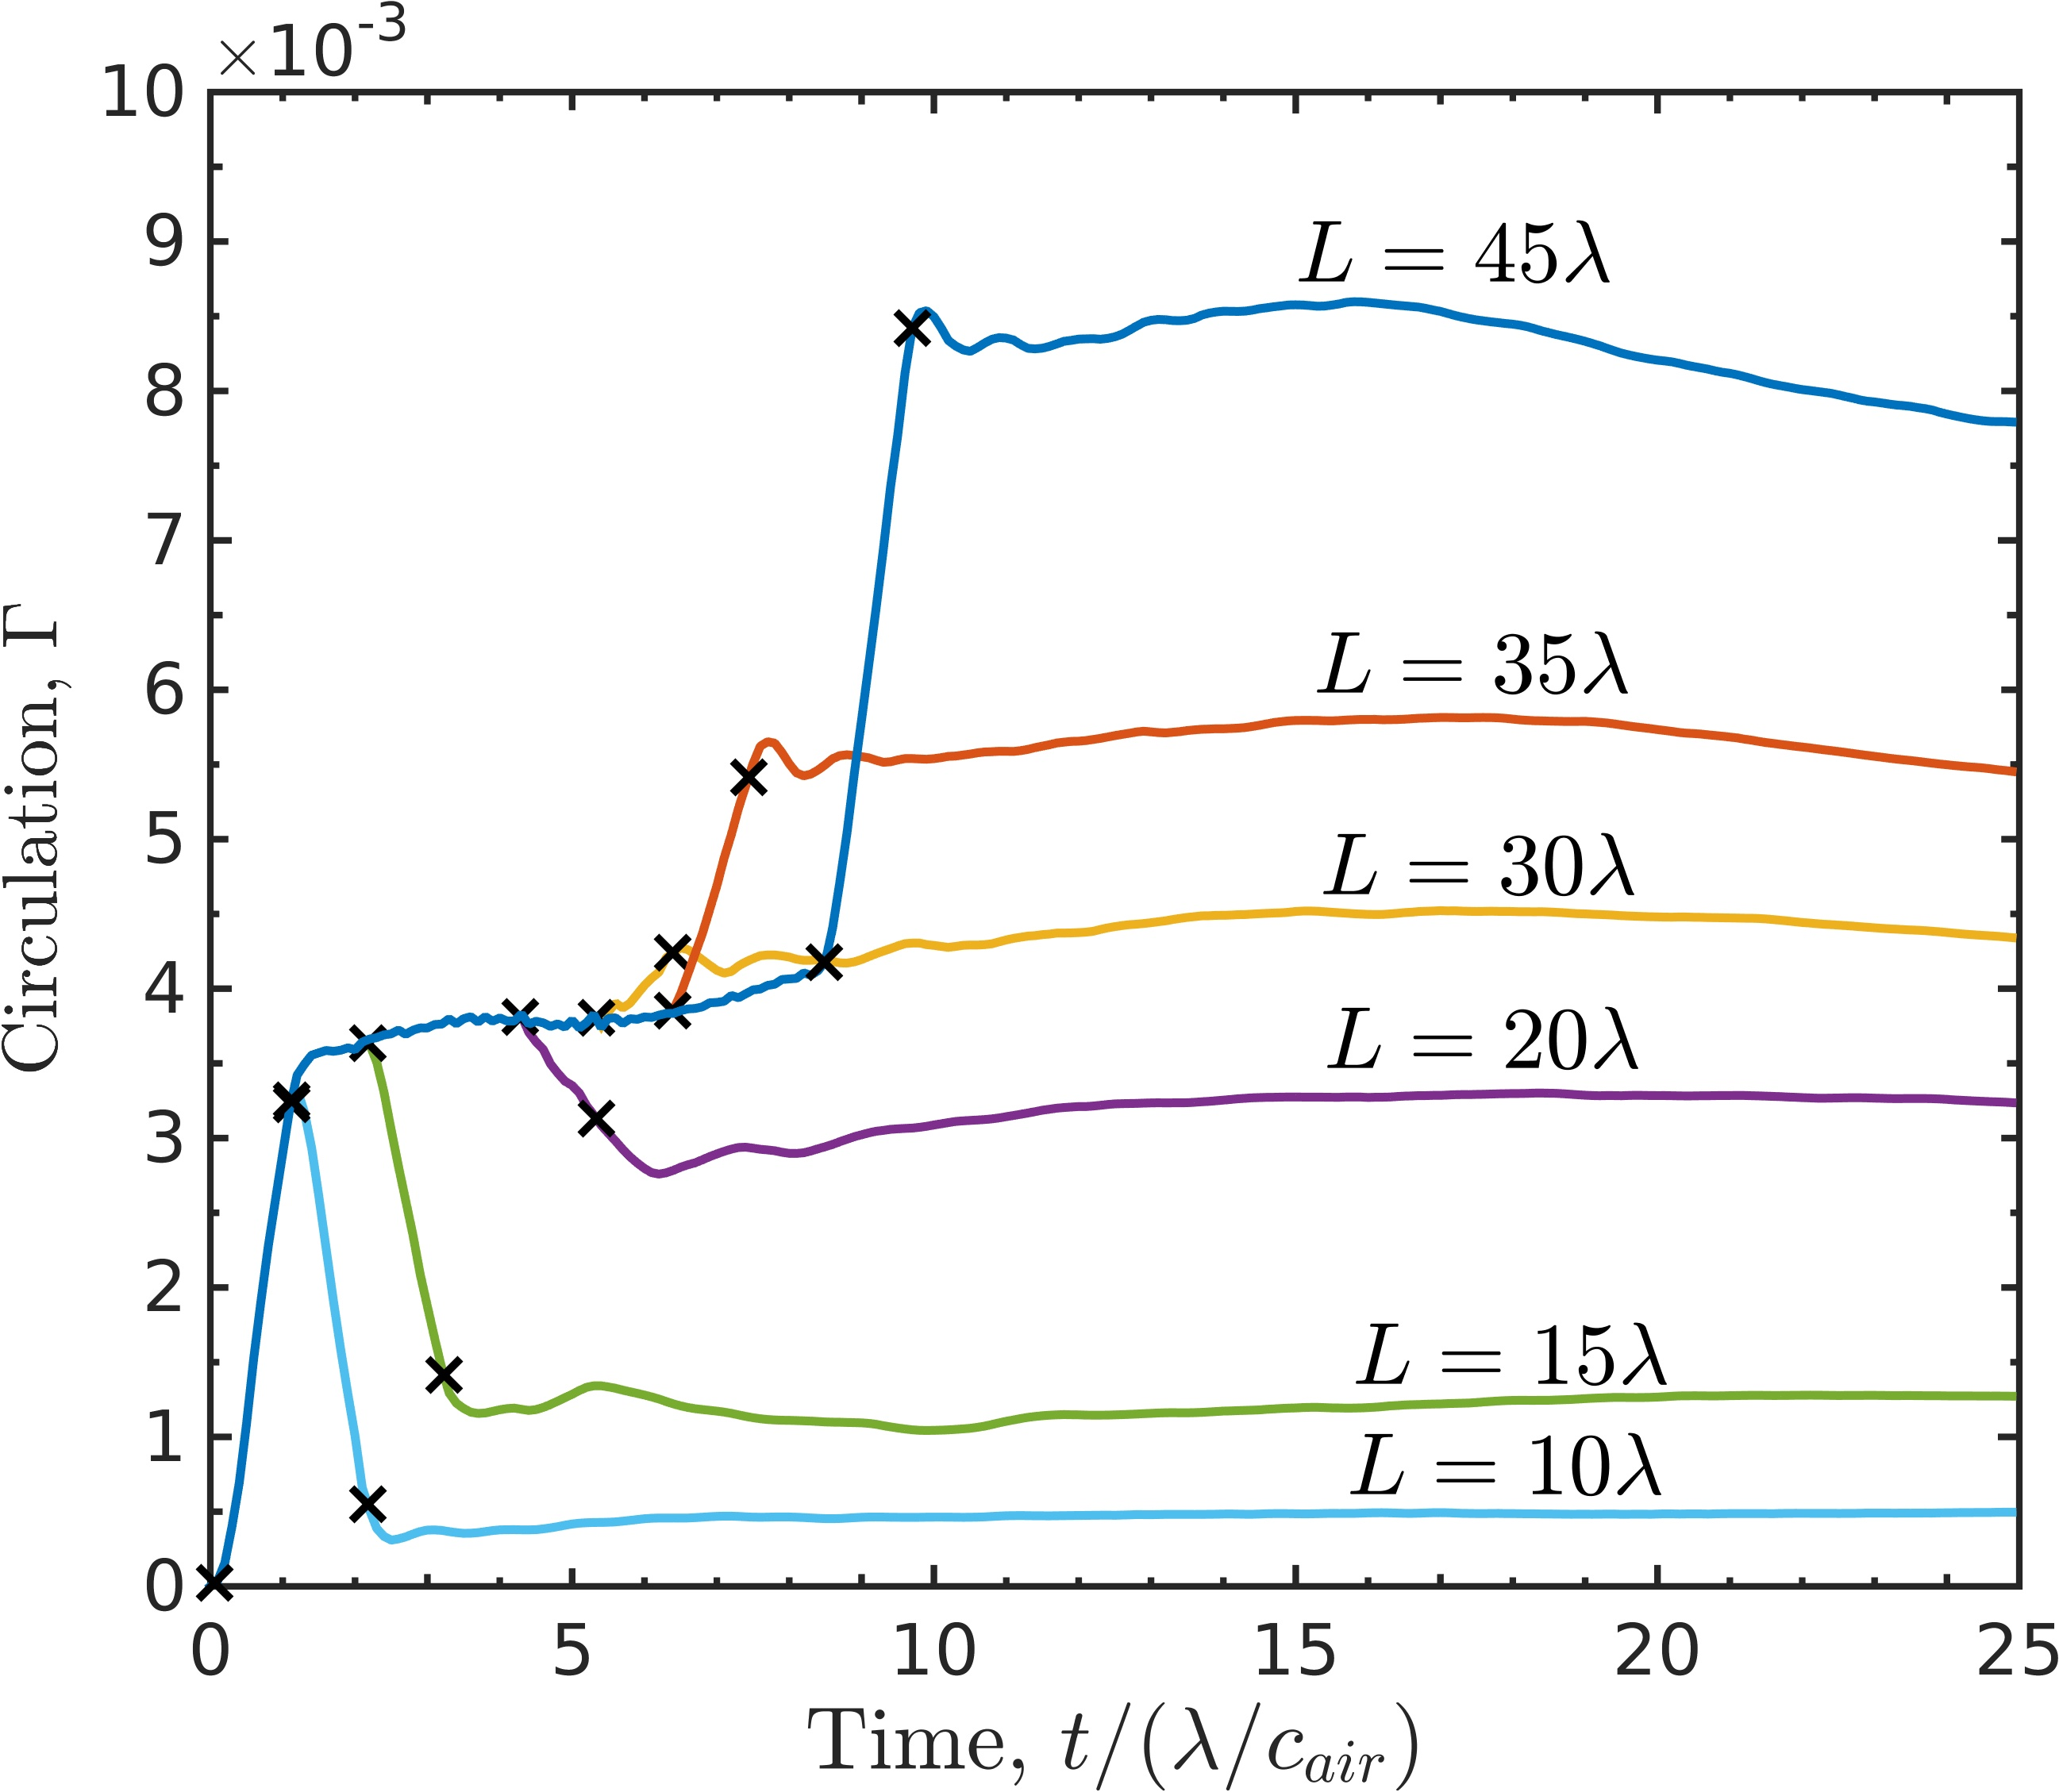
\includegraphics[width=0.48\textwidth]{./figs/lung_figs/circulation_multi-lag_fixed}
  \caption[The interface and circulation dependence on wave
  duration]{The interface amplitude (left) and circulation (right)
    histories for waves of varying total length $L$ and elevated
    static pressure duration between the expansion and compression
    . Here we show results for $L=45\lambda$ (blue), $L=35\lambda$
    (orange), $L=30\lambda$ (yellow), $L=20\lambda$ (purple),
    $L=15\lambda$ (green), $L=10\lambda$ (light blue)}
  \label{fig:trapz_circ_interface_multi-lag}
\end{figure}
%
\subsection{Discussion}
\label{subsec:discussion}
After the passage of the trapezoidal acoustic waves the pressure
returns to the initial, ambient conditions. This implies that the
integral of the pressure gradient $\nabla p$ along the interface, over
all time is zero. Hence we surmise that if the interface remains
unchanged during the interaction with the wave, as it would for a wave
moving with infinite velocity, $\nabla \rho$ would remain constant and
the net baroclinic circulation deposited must be zero. Thus for any
finite duration acoustic wave to deposit net baroclinic circulation
upon an interface, the interface itself must deform during interaction
with the wave. This deformation alters the misalignment of the
pressure and density gradients throughout the passage of the wave such
that vorticity deposited by the compression and expansion waves do not
cancel. Note that this of particular interest for waves in which
the pressure returns to the initial condition after the wave passes,
which is not the case for the traditional shock-accelerated \ac{RMI}
problem.

For the cases varying the length of the wave $L$, we previously noted
that whether the expansion increased or decreased the total
half-domain circulation depended on whether it encountered the
interface before or after the phase change. If indeed circulation is
driving the deformation of the interface, then changes in the waveform
that appear to have very little effect on the interface dynamics
during the wave-interface interaction period, may have far more
significant impacts on the long term dynamics of the interface via
vorticity.

%% Local Variables:
%%% mode: latex
%%% TeX-master: "../main"
%%% End:


\section{Results and discussion}%
\label{sec:results}%
% 
\subsection{Qualitative observations of the interface response to the trapezoidal wave}
\label{subsec:Qualitative}
We consider an acoustic wave initially in water, that propagates in
the $-y$-direction toward the water-air interface at $t = 0^+$. As a
base reference case we consider a trapezoidal wave with $p_a = 10$ MPa
(See Figure \ref{fig:p0}). Upon interaction with the interface, nearly
all of the acoustic energy is reflected back into the water as a
tensile wave due to the decrease in acoustic impedance across the
interface. The transmitted wave is weakly focused or defocused,
depending on the convex or concave nature of the curved interface. Both the
reflected and transmitted waves leave the domain at the inflow and outflow
boundaries.
% 
\begin{figure}
  \centering
  % \  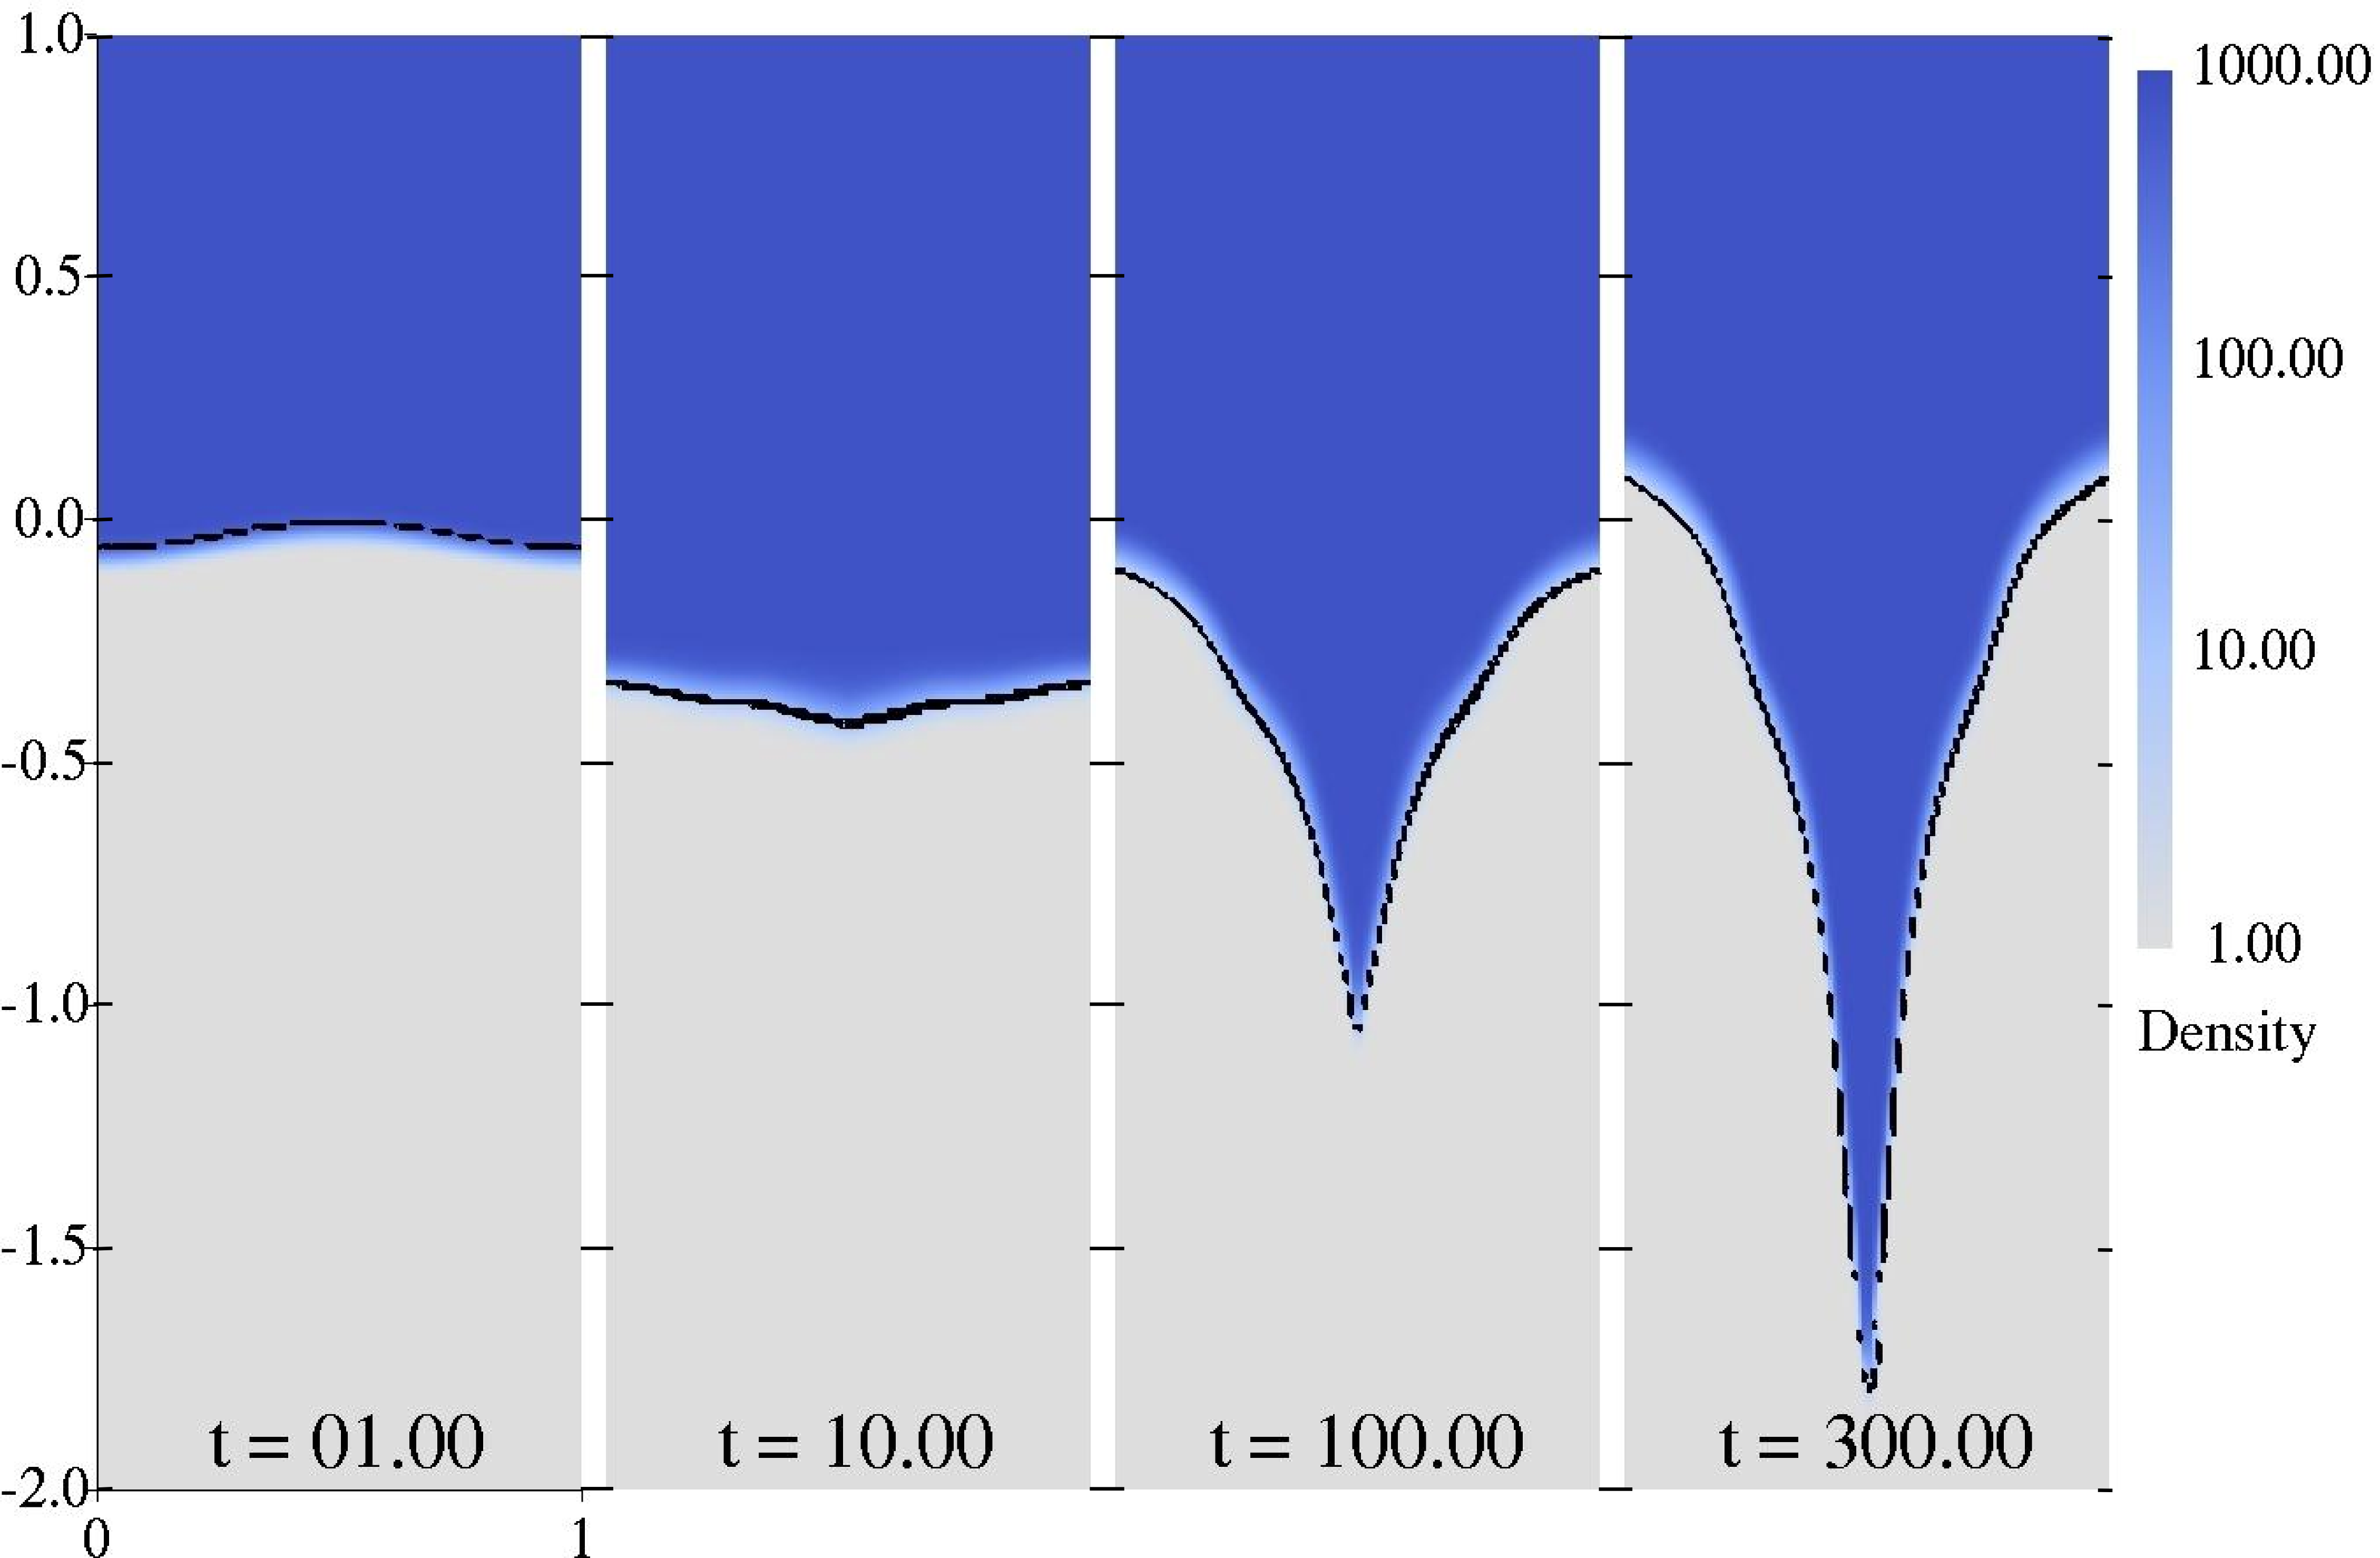
\includegraphics[width=0.9\textwidth]{./figs/lung_figs/snapshots_density_t1}
  \def\svgwidth{0.95\textwidth}
  \import{./figs/lung_figs/}{snapshots_density_t1_wnd_2017-05-23.pdf_tex}
  \caption[The evolution of the acoustically perturbed interface]
  {The evolution of the interface during and after the interaction
    with the wave is illustrated. Contour plots of density at
    $t=4.7, 47.5, 475, 1424$, %$t=1, 10, 100, 300$,
    for the baseline $p_a = 10$ MPa trapezoidal wave. Water (Blue);
    Air (grey); and constant volume fraction of water $\alpha=0.5$
    (black line) are indicated.}
  \label{fig:interface_snapshots}
\end{figure}
% 
Figure \ref{fig:interface_snapshots} illustrates the evolution of the
interface. Contour plots of the density during the
compression-interface interaction $(t = 4.7)$, shortly after the wave
leaves the interface $(t = 47.5)$, and at late times $(t = 475, 1424)$ are
shown. The interface perturbation grows from an initially smooth
sinusoid to a sharp spike at late times, long after all waves have
left the domain.
% 
\begin{figure} 
  \centering
  \begin{subfigure}[b]{0.45\textwidth}
    \centering
    % 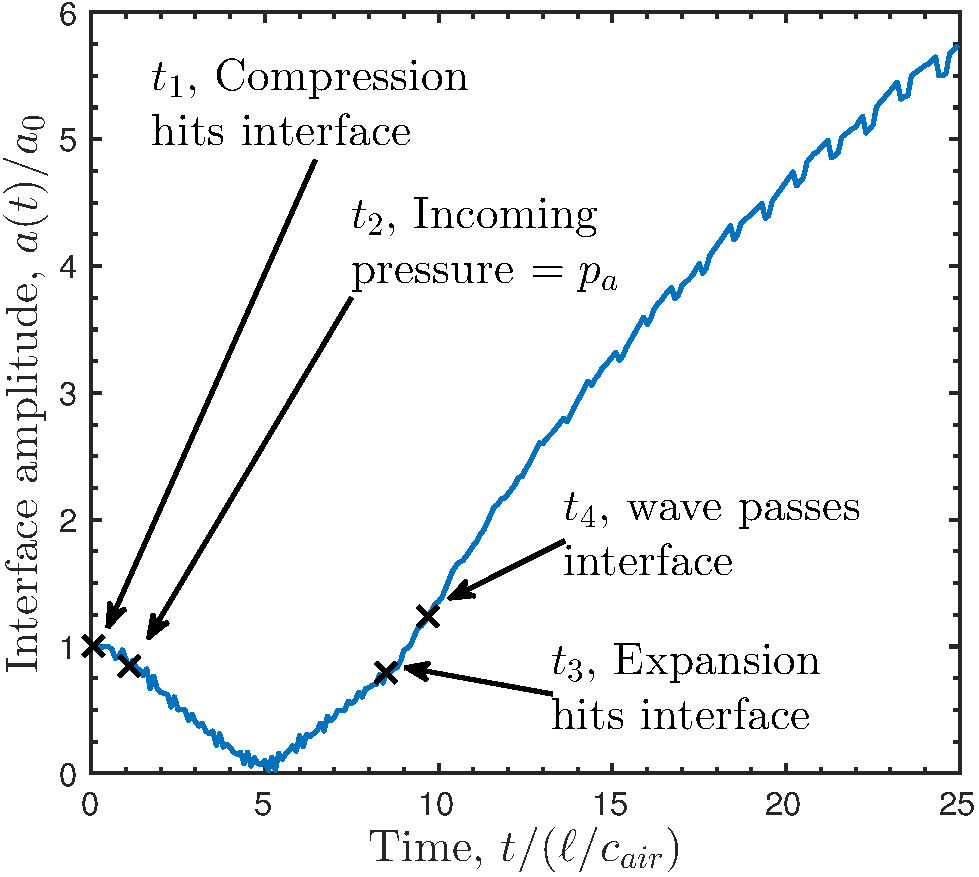
\includegraphics[width=\textwidth]{./figs/lung_figs/trapz10_intf_schematic.pdf}
    \includegraphics[width=\textwidth]{./figs/lung_figs/trapz10_intf_schematic_24-May-2017.pdf}
    \caption{\label{fig:trapz10_interface25} $0 \leq t/(\ell/c) \leq 120$.}
  \end{subfigure}
  ~
  \begin{subfigure}[b]{0.45\textwidth}
    \centering
    \includegraphics[width=\textwidth]{./figs/lung_figs/trapz10_intf_t1000_24-May-2017.pdf}%
    \caption{\label{fig:trapz10_interface1000} $0 \leq t/(\ell/c) \leq 5000$.}
  \end{subfigure}
  \caption[Interface perturbation amplitude history for $p_a = 10$ MPa
  trapezoidal wave]{The interface perturbation amplitude history
    $a(t)$ is shown for the baseline $p_a = 10$ MPa trapezoidal wave
    case, for $t \leq 120$ \protect\subref{fig:trapz10_interface25}
    and $t \leq 5000$ \protect\subref{fig:trapz10_interface1000}. The
    times at which different stages of the incoming trapezoidal
    pressure wave encounter the interface are indicated as $t_1$: the
    compression; $t_2$: the static elevated pressure $p_a$; $t_3$: the
    expansion; $t_4$: the return to ambient pressure.}
  \label{fig:trapz10_interface}
\end{figure}\par
% 
We examine the time evolution of the perturbation growth driven by the
wave interaction in Figure \ref{fig:trapz10_interface}. The initial
condition is such that the time axis origin coincides approximately
with the leading end of the wave impinging upon the interface. The
early time behavior (Figure \ref{fig:trapz10_interface25}) is
characterized by several distinct events. Following the impingement of
the leading end of the wave at $t_1=0^+$, the pressure at the interface
increases until $t_2\approx5.2$, at which point the pressure has reached its
maximum amplitude. The interface amplitude decreases to nearly zero
and starts to grow again thereafter. The pressure remains constant
until $t_3\approx40$, at which point the leading end of the rarefaction reaches
the interface. The pressure decreases until $t_4\approx47$, at which point the
full wave has left the interface and the pressure is atmospheric
again, as it was originally. Well after the wave has passed, the
perturbation amplitude continues to grow, reaching many times its
initial value. At these late times, the growth appears to smooth,
continuous and monotonic, such that it may obey a power-law dependence
on time.
% 
%%%%%%%%%%%%%%%%%%%%%%%%%%%%%%%%%%%%%%%%%%%%%%%%%%%%%%%%%%%%%%%%%% 
%%%%%%%%%%%%%%%%%%%%%%%%%%%%%%%%%%%%%%%%%%%%%%%%%%%%%%%%%%%%%%%%%% 
%%%%%%%%%%%%%%%%%%%%%%%%%%%%%%%%%%%%%%%%%%%%%%%%%%%%%%%%%%%%%%%%%% 
%%%%%%%%%%%%%%%%%%%%%%%%%%%%%%%%%%%%%%%%%%%%%%%%%%%%%%%%%%%%%%%%%% 
% 
\subsection{Vorticity and circulation dynamics}
\begin{figure}
  \centering
  % 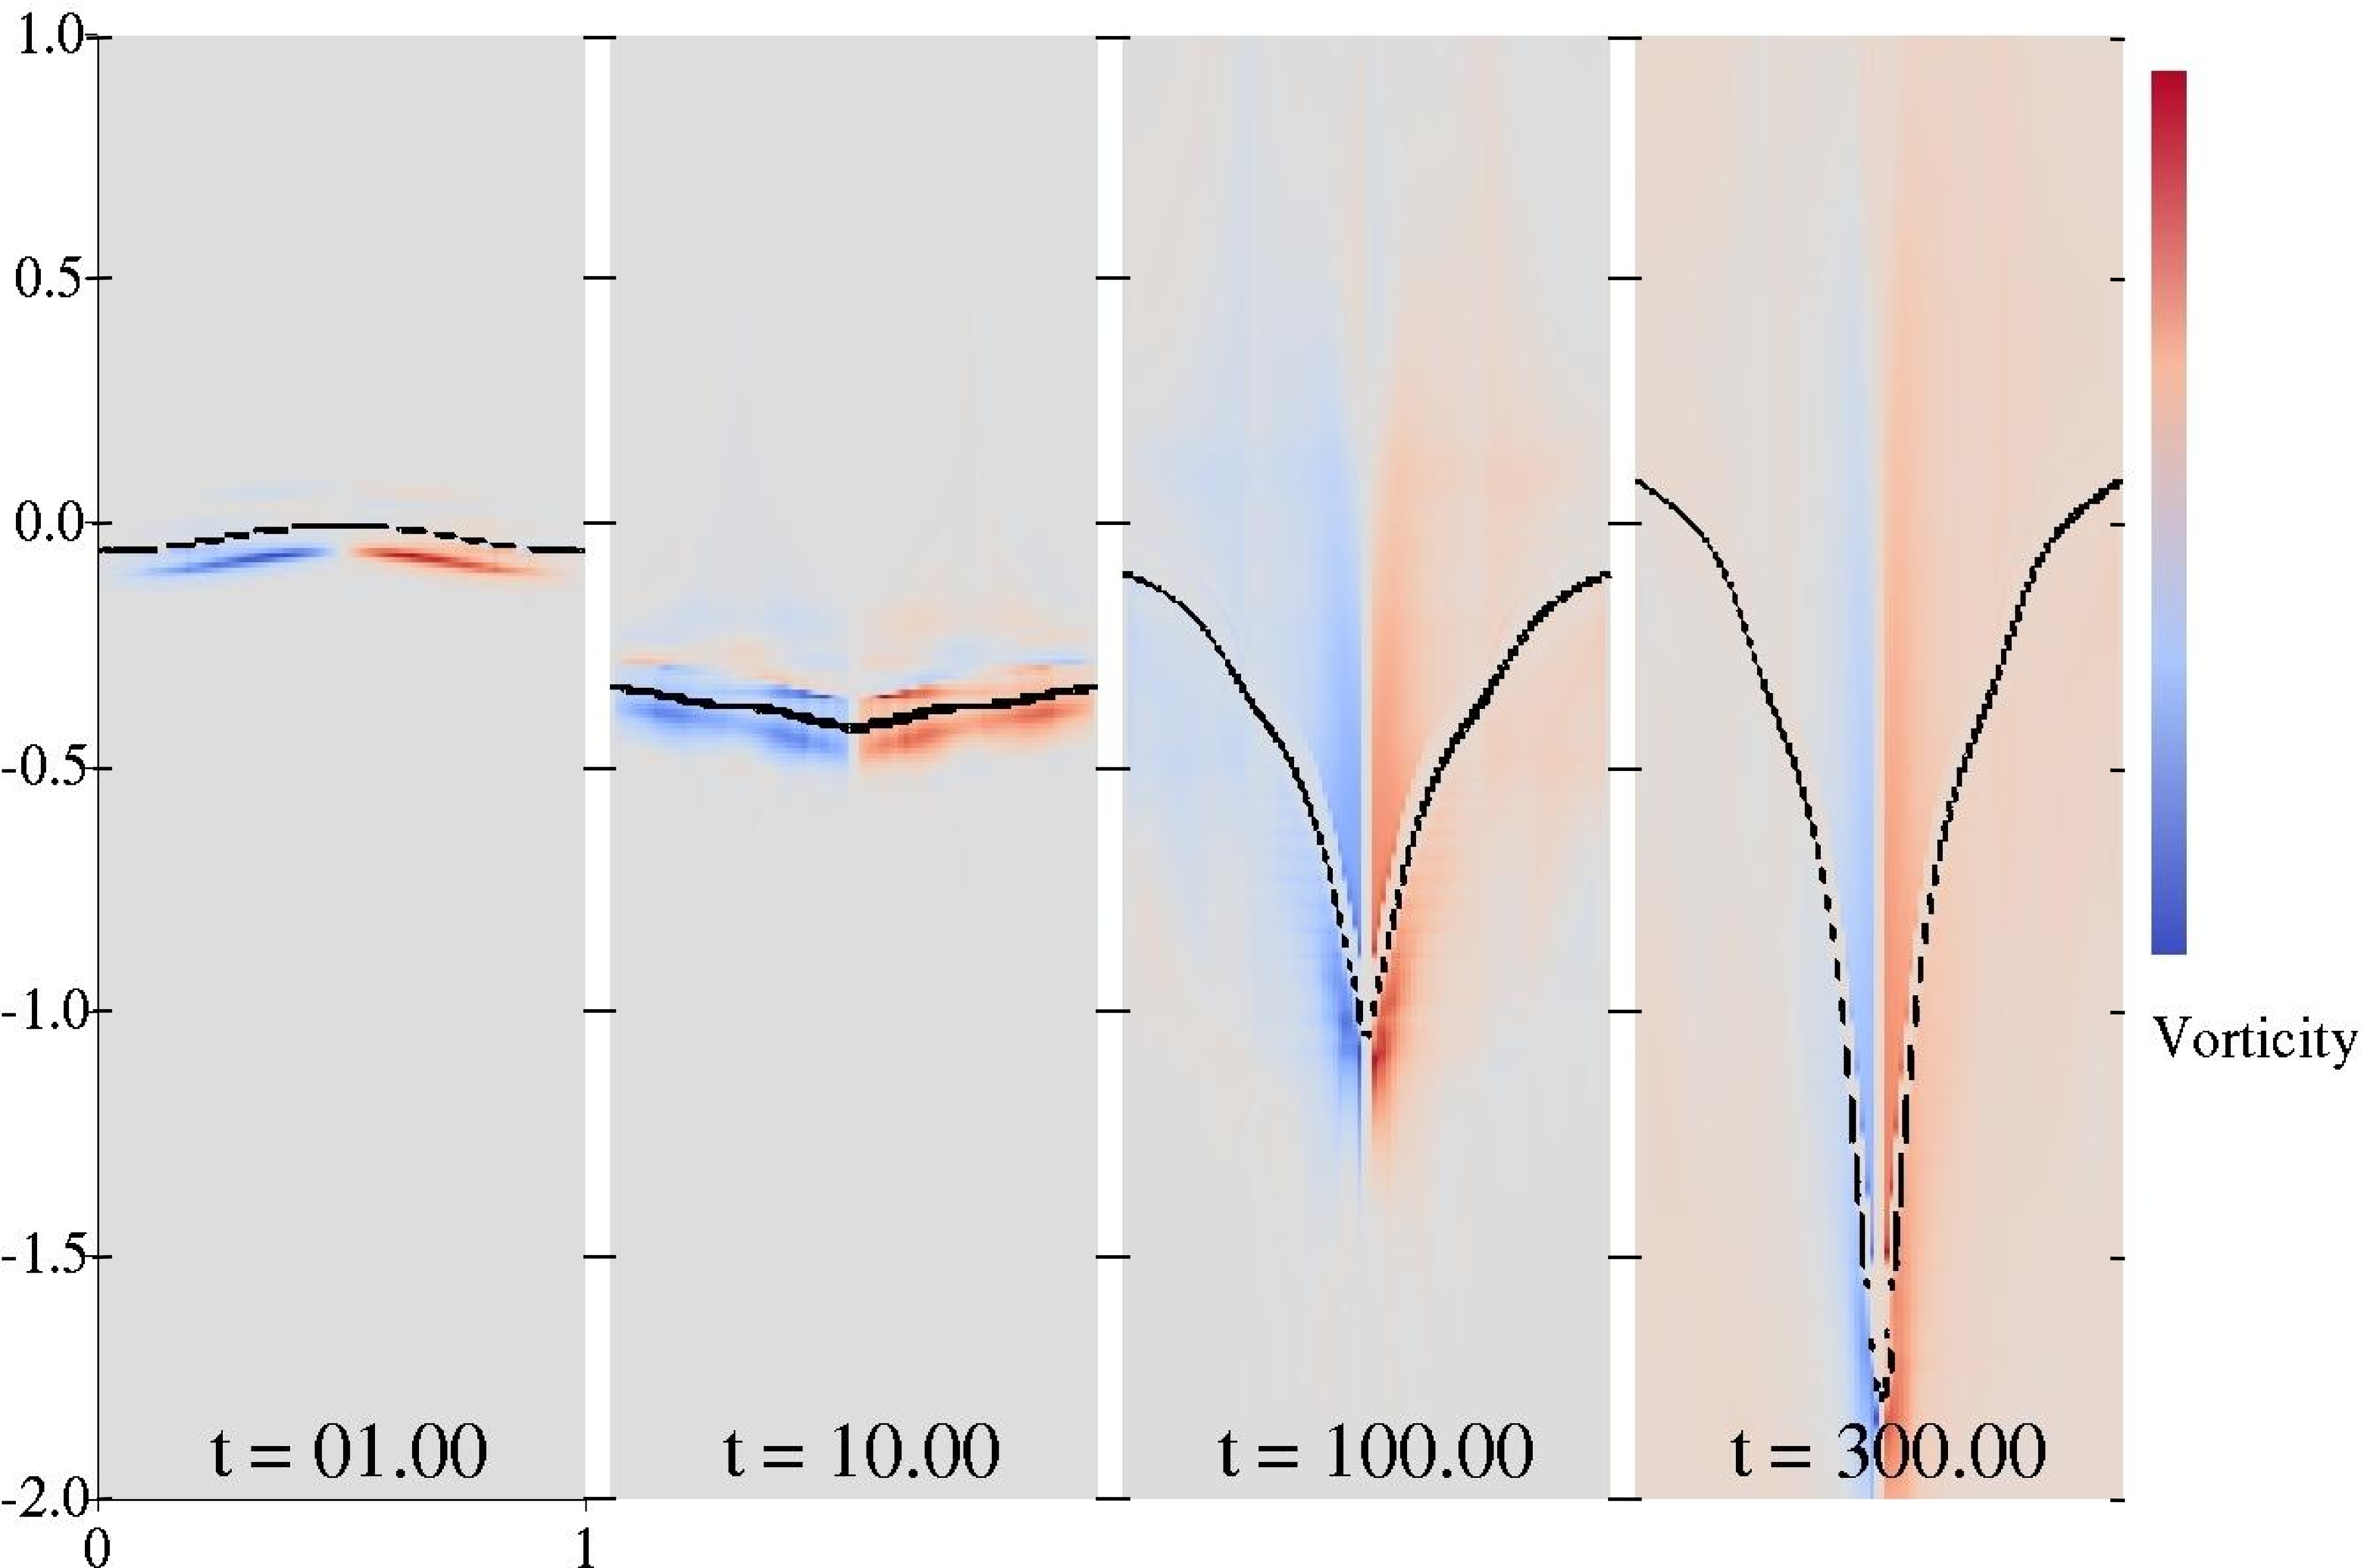
\includegraphics[width=0.9\textwidth]{./figs/lung_figs/snapshots_vorticity_t1}
  \includegraphics[width=0.98\textwidth]{./figs/lung_figs/vorticity_snapshot_fixcbar_mat_24-May-2017}
  \caption[The evolution of the vorticity] {The evolution of the
    vorticity field is illustrated. Contour plots of vorticity are
    shown for the baseline $p_a = 10$ MPa trapezoidal wave case at
    $t = 4.75, 47.5, 475, 1424$. Constant volume fraction of water
    $\alpha = 0.5$ contour lines are indicated in black.}
  \label{fig:vorticity_snapshots}
\end{figure}
% 
The perturbation growth can be understood in terms of
vorticity. Figure \ref{fig:vorticity_snapshots} shows contour plots of
the vorticity field at $t = 4.75, 47.5, 475, 1224$, for the baseline
$p_a = 10$ MPa trapezoidal wave case. At $t = 4.75$, near the end of the
compression-interface interaction, a vortex sheet exists along the
interface. Given the interface-capturing approach, the interface
numerically diffuses over a few computational cells such that
vorticity is primarily concentrated in the air. This vorticity drives
the interface deformation after the passage of the wave. By $t = 48$ the
expansion end of the wave has passed. Since the interface is no longer
a smooth sinusoid but is corrugated, vorticity of both signs is
deposited by the wave. As the interface deforms, bubbles of light
fluid rise upwards and spikes of dense fluid fall. The vorticity
concentrates along the spike. Even at late time, the vorticity is
largely concentrated along the interface.

The vorticity dynamics are described by the vorticity equation,
written here for two-dimensional flows,
\begin{align} \label{eq:vorticity_euler}
  \frac{\partial \boldsymbol{\omega}}{\partial t}+\left(\boldsymbol{u}\cdot\nabla\right)\boldsymbol{\omega} =% 
  - \boldsymbol{\omega}\left(\nabla\cdot\boldsymbol{u}\right) + \frac{\nabla\rho\times\nabla p}{\rho^2},%
\end{align}
where $\boldsymbol{\omega}$ is the vorticity. The temporal and spatial
evolution of vorticity (left-hand side) is governed by dilational
changes and baroclinic vorticity. The high impedance mismatch and
relatively low dilation at the wave amplitudes of interest make the
first term on the right-hand side essentially negligible compared to
the baroclinic term, given the nearly discontinuous density gradient
and the significant pressure variations over relatively short
lengths. Appendix \ref{sec:oom_analysis} quantitatively demonstrates
that the vorticity production is dominated by the baroclinic term. In
the following sections, we investigate the relation between the
vorticity dynamics and the perturbation growth.

\subsubsection{Circulation deposition}
As an intergral measure of vorticity, we consider the circulation
produced in the right-half domain (the left is equal and opposite by
symmetry) for the baseline case in Figure
\ref{fig:trapz10_circ_schematic}%
\begin{figure}
  \centering
  \begin{subfigure}[b]{0.48\textwidth}
    \centering
    \includegraphics[width=\textwidth]{./figs/lung_figs/trapz10_circ_schematic_24-May-2017.pdf}
    \caption{\label{fig:trapz10_circ_schematic_t25} $0 \leq t \leq 120$ }
  \end{subfigure}
  ~
  \begin{subfigure}[b]{0.48\textwidth}
    \centering
    \includegraphics[width=\textwidth]{./figs/lung_figs/Gamma_t1000_24-May-2017.pdf}
    \caption{\label{fig:trapz10_circ_schematic_t1000} $0 \leq t \leq 5000$}
  \end{subfigure}
  % 
  \caption[Circulation deposition by the $p_a = 10$ MPa trapezoidal
  wave] {The circulation history for the right-half domain is shown
    for the baseline $p_a = 10$ MPa trapezoidal wave case for
    $t \leq 120$ \protect\subref{fig:trapz10_circ_schematic_t25} and
    $t \leq 5000$
    \protect\subref{fig:trapz10_circ_schematic_t1000}. The times at
    which different stages of the incoming trapezoidal pressure wave
    encounter the interface are indicated as $t_{1-4}$.}
  \label{fig:trapz10_circ_schematic}
\end{figure}
% 
Figure \ref{fig:trapz10_circ_schematic}, shows circulation history of
the right-half domain for the baseline $p_a = 10$ MPa wave case for $t \leq 120$, during
and shortly after the wave-interface interaction, and for the duration
of the simulation, $t \leq 5000$. The points at which different
components of the wave encounter the interface are indicate as
$t_{1-4}$, as described in section \ref{subsec:Qualitative}.

From $t_1$ to $t_2$, positive vorticity (circulation) is deposited
given the misalignment between the density and pressure
gradients. From $t_2$ to $t_3$ the pressure gradient is essentially
zero, but the interface is still deforming due to the vorticity
deposited by the compression. The circulation remains nearly constant
during this time interval; the small changes are due to waves
reflecting in the traverse direction as the interface is
deforming. The initial peak (at $x=0.5\ell$) moves downward while the
initial troughs at $x=0$ and $1\ell$ move upward, such that the phase
of the perturbation inverts at $t \approx 24$. From this point on, the
density gradient along the right hand side of the interface no longer
points toward the top-right, but toward the top-left. At $t_3$ the
expansion wave starts to interact with the interface. Although the
pressure gradient has inverted, the direction of the density gradient
after phase inversion is such that baroclinic vorticity \emph{of the
  same sign} is deposited. At $t_4$ the ultrasound wave has finished
traversing the interface and ceases depositing vorticity along the
interface. The circulation then decreases before steadily increasing
over time. The decrease occurs as a consequence of the vorticity being
initially concentrated more heavily in the lighter, more gaseous
portion of the interface region. As the vorticity mixes the light and
heavy fluid along the interface, the rotational energy spreads into
the heavier fluid. As vorticity is a kinematic metric and is not
conserved, the total circulation decreases such that energy is
conserved. The rise in vorticity that follows appears to be secondary
baroclinic vorticity generated by the acceleration fields producing
pressure gradients misaligned with the density gradient along the
interface. This can be shown using the methods provided for
calculating individual physical contribution to circulation in
Appendix \ref{sec:oom_analysis} and pressure and density contours of
the domain (not shown here).

\subsubsection{Early circulation-driven interface growth}
\label{subsubsec:tgamma}
\begin{figure}
  \centering
  \captionsetup[subfigure]{labelformat=empty}
  \begin{subfigure}[t]{0.45\textwidth}
    \centering
    \includegraphics[height=0.8\textwidth]{./figs/lung_figs/trapz10_bubble-spike_location_01-Jun-2017}
    \caption{Bubble and spike location}
  \end{subfigure}
  % \begin{subfigure}[t]{0.45\textwidth}
  %   \centering
  %   \includegraphics[height=0.8\textwidth]{./figs/lung_figs/trapz10_bubble-spike_location_t1000_24-May-2017}
  %   \caption{Bubble and spike location}
  % \end{subfigure}
  \caption{The $y$-locations of the bubble and spike are shown for the
    baseline $p_a = 10$ MPa trapezoidal wave case, for $t \leq
    120$. By definition, the bubble is the top curve and the spike is
    bottom.}
  \label{fig:trapz10_bs_location}
\end{figure}
Throughout the wave-interface interaction, the evolution of the
interface is driven by both the acoustic velocity and baroclinic
vorticity deposited by the wave. The effects of vorticity can be
observed relatively early on. As previously explained, from $t_2$ to
$t_3$ the interface experiences acoustic pressure and velocity that
are approximately constant in time and uniform in the
$x$-direction. Linear acoustics explains the downward motion of the
interface during this time. However, as seen in Figure
\ref{fig:trapz10_circ_schematic_t25}, the interface perturbation
decreases amplitude, inverts phase, and then increases amplitude
during this period as well. This deformation cannot be explained by
linear acoustics, but can be easily explained as a result of
baroclinic vorticity observed at the interface.

The interplay between the acoustic and vorticity mechanisms driving
the interface is useful to understand when attempting to analyze and
explain the dynamics of the flow. At some point during the wave
interface interaction, as the acoustic amplitude decreases and
baroclinic vorticity increases, the baroclinic vorticity overcomes the
acoustic pressure and becomes the dominant mechanism driving the
growth. We will define at time $t_\Gamma$ as the earliest point, in
which we can be certain we have entered this regime. At this point we
can begin analyzing the evolution of the interface in terms of
circulation and vorticity.

After the wave has passed, baroclinic vorticity is the only remaining
mechanism to drive the deformation of the interface, so intuitively
$t_\Gamma \leq t_4$. To determine $t_\Gamma$ more precisely, we
consider the physical mechanisms driving the bubble and spike during
the wave-interface interaction. Figure \ref{fig:trapz10_bs_location}
shows the $y$-location of the bubble and spike for the $p_a = 10$ MPa
trapezoidal wave case. By definition, the bubble is the top curve and
the spike is bottom curve. At $t = 44.6$ (indicated by the black
dotted line), in approximately the middle of the expansion-interface
interaction, the nature of the bubble and spike velocities appear to
change simultaneously. The bubble (located at $x = 0, 1\ell$) reverses
direction and begins moving upward; simultaneously, the spike (located
at $x = 0.5\ell$) continues to move downward, but at a noticeably
slower velocity. Plots of pressure and volume fraction as a function
of $y$ at $x=0.5$ and $1$ (not shown here) reveal that at this time,
both the bubble and the spike experience a negative pressure gradient
in the upper portion of the interface region
$(0.65 \leq \alpha < 1.0)$ and approximately zero pressure gradient
throughout the remainder of the interface region
$(0 \leq \alpha < 0.65)$. From linear acoustics alone, we would expect
an upward motion for both the bubble and the spike. However the
divergence of the two, and specifically the upward motion of the
bubble, suggest that the acoustic velocity is no longer dominating the
vertical movement of the bubble and spike. However, the observed
motion is exactly what one would expect from the opposing vortex
pairs which surround the bubble and spike. This suggests that by this
point in time, vorticity has become the dominant mechanism driving the
bubble and spike, and as such we define $t_\Gamma$ as the point,
during the wave-interface interaction when the bubble and spike first
begin to diverge. For the $10$ MPa trapezoidal wave case shown here,
$t_\Gamma=44.6$.
%
%At $t_\Gamma=9.4$ nearly the entire interface region
%$(\alpha \leq 0.98)$ is subject to positive pressure.
% At $t_\Gamma=9.4$ $(\alpha \geq 0.65)$ is subjected to negative pressure gradient in y-direction.
% $(\alpha < 0.65)$ is subjected to no pressure gradient in y-direction.
%
\subsubsection{Circulation-driven, late-time growth of the interface}
\begin{figure}
  \centering
  \begin{subfigure}[t]{0.45\textwidth}
    \centering
    \includegraphics[height=0.8\textwidth]{./figs/lung_figs/a0_t1000_24-May-2017}
    \caption{\label{fig:trapz_interface_t1000} Interface amplitude: $a(t)/a_0$}
  \end{subfigure}
  ~
  \begin{subfigure}[t]{0.45\textwidth}
    \centering
    \includegraphics[height=0.8\textwidth]{./figs/lung_figs/Circulation_t1000_24-May-2017}
    \caption{\label{fig:trapz_circ_t1000} Circulation amplitude: $\Gamma/\ell c$}
    % \caption[The circulation long time]{The circulation histories
    % $\Gamma(t)$ corresponding to the $p_a = 5$ (blue), $7.5$ (red), $10$
    % (green), and $12.5$ (Purple) MPa trapezoidal waves are shown for
    % $t\leq 1000$. }
    \label{fig:trapz_circ_t1000}
  \end{subfigure}
  % 
  \caption[The interface amplitude and circulation for long time and
  multiple wave amplitudes]{The interface amplitude
    \subref{fig:trapz_interface_t1000} and circulation
    \subref{fig:trapz_circ_t1000} histories are shown for trapezoidal wave cases 
    $p_a = 5$ (blue), $7.5$ (red), $10$ (green), and $12.5$ (Purple) MPa, for $t \leq 5000$.}
  \label{fig:trapz_interface_acirc}
\end{figure}

\begin{table}[ht]
\centering
\caption{Circulation during the wave-interface interaction}
\label{tab:circ}
\begin{tabular}[t]{L{0.15\linewidth} L{0.1\linewidth} L{0.1\linewidth} L{0.1\linewidth} L{0.1\linewidth} }
\toprule
&\multicolumn{4}{c}{$\Gamma(t_i)/(\ell c_{water}) \times 10^{4}$}\\
$p_a$ (MPa) &$t_1$&$t_2$&$t_3$&$t_4$\\% t = 0, 5.22,40.36,47.00
\midrule
5.0&0&3.3&3.8&2.9\\
7.5&0&5.0&6.0&8.7\\
10.0&0&6.8&8.8&18.0\\
12.5&0&8.5&11.9&30.5\\
\bottomrule
\end{tabular}
\end{table}%
\begin{comment} %time [circ (t1-4)]
5.00 MPa         0    0.0000    0.3349    0.3834    0.2949
7.50 MPa    5.2227    0.0000    0.5041    0.6006    0.8704
10.0 MPa   40.3573    0.0000    0.6758    0.8814    1.7981
12.5 MPa   47.0044    0.0000    0.8529    1.1856    3.0511
\end{comment}
Section \ref{subsec:Qualitative} clearly demonstrates that the
perturbation amplitude grows well after the incident ultrasound wave
has traversed the interface. Such a growth may have significant
implications when considering ultrasound-generated damage on the lung
as the alveolar surface may elongate, potentially until rupture of
capillaries. Here, we are interested in predicting this late-time
perturbation growth.

This growth is driven by the baroclinic vorticity deposited by the
interaction of the ultrasound wave with the interface. It is therefore
reasonable to expect the growth rate to increase if more vorticity is
deposited. A reasonable measure of the magnitude of vorticity is the
circulation (in one half of the domain as that in the other half is
equal and opposite). In the present problem, the relevant variable of
interest is the wave amplitude; wave length is another one that will
be considered in Section \ref{subsubsec:transient}. Since the
baroclinic term is proportional to the pressure gradient, the
circulation is expected to increase with increasing wave pressure
amplitude, and so is the perturbation amplitude. Figure
\ref{fig:trapz_interface_acirc} shows the time history of the
perturbation amplitude and circulation in the right-half plane for
different wave pressure amplitudes. As expected, the perturbation
growth rate increases with increasing pressure amplitude in a fashion
that appears monotonic. At late times, the data suggests that the
growth may be reaching an asymptotic rate. In all cases, the
circulation reaches a peak value at the time the wave has finished
traversing the interface; thereafter, the circulation decreases before
reaching a plateau (for $p_a = 5.0$ and $7.5$ MPa) or steadily increasing
(for $p_a = 10$ and $12.5$ MPa). While the peak circulation at $t_4$ and the
late-time circulation magnitude both exhibit similar dependence on the
pressure amplitude, the decrease immediately after the wave has left
the interface behaves in a very different fashion for $5$ MPa, where
the decrease and recovery are much faster. This due to the phase
inversion occurring during as the expansion wave encounters the
interface for the $p_a = 5$ MPa case, aligning the pressure and density
gradients such that the incoming expansion deposits little vorticity.

We now determine whether there is a universal rule governing the
perturbation growth $a$ in time $t$. Clearly, the perturbation will
depend on the circulation, $\Gamma$. As the perturbation grows, it is
expected that the vorticity becomes redistributed along the interface,
such that there may be a dependence on the instantaneous interface
length $s$, as well as the initial wavelength $\ell$. Finally, given
that the wave takes a finite duration to traverse the interface,
dependence on the sound speed of the water $c$ is expected. Thus, the
dependence of the amplitude on these variables can be formulated as a
dimensional analysis problem as follows:
\begin{align}
  \label{eq:dimensional_amplitude}
  a(t)=f(\Gamma, s, \ell, c; t) \quad \Rightarrow \frac{a(t)}{\ell} = F\left(\frac{\Gamma}{\ell c}, \frac{s}{\ell}; \frac{t}{\ell/c}\right),
\end{align}
where $\ell$ and $c$ are used for non-dimensionalization.

Once the wave has traversed the interface, there is no significant
mechanism to affect the circulation (except in the $p_a = 12.5$ MPa
case). However, as the interface deforms and elongates (i.e., $s(t)$
increases), the vorticity gets redistributed along the interface. As
suggested by \hl{[add references about Sam's vortex sheet model]}, the
circulation density $\Gamma / s$ is the relevant driver for the
interface dynamics. As observed in Section \ref{subsubsec:tgamma},
baroclinic vorticity begins to dominate the motion of the interface at
$t_\Gamma$. Thus, we expect the perturbation amplitude to depend on
this quantity taken at the instant when growth is dominated by
baroclinic vorticity, $\Gamma(t_\Gamma)/s(t_\Gamma) = \Gamma_0 /
s_0$. It therefore follows that
% 
\begin{align}
  \label{eq:dimensionless_groups}
  \frac{a(t)}{\ell}=G\left(\frac{\Gamma_0}{s_0 c}, \frac{t c}{\ell} \right).
\end{align}
% 
As suggested by the observed behavior in Figure
\ref{fig:trapz_Interface_acirc} and Table \ref{tab:circ}, we hypothesize
that the perturbation growth scales linearly with the circulation
density, such that
% 
\begin{align}
  \label{eq:dimensionless_relationship}
  \frac{a(t)}{\ell}=\frac{\Gamma_0}{s_0 c}\mathcal{F}\left(\frac{t c}{\ell} \right).
\end{align}
% 
To test this hypothesis, we scale $a(t)$ by the circulation density in
Figure \ref{fig:trapz_interface_t1000_scaled}. To facilitate the
comparison, the time origin has been shifted such that the instant the 
phase inverts occurs simultaneously in each case. Two observations
stand out. First, the scaled growths collapse onto what appears to be
a single curve. Second, this curve appears to asymptote to a constant
slope in this logarithmic plot, thus indicating a power-law
behavior. To compute the time exponent $n$, we write
\begin{align}
  \label{eq:log_a}
  \ln\left[(a(t-t_p) / \left(\frac{\Gamma_0}{s_0}\frac{\ell}{c}\right)\right] = b + n\ln\left[(t-t_p)/(\ell/c)\right],
\end{align}
where $t_p$ is the time of phase reversal and $b$ is the $y-$intercept
of the best fit line, which depends on the value of
$(a(t-t_p) / \left(\frac{\Gamma_0}{s_0}\frac{\ell}{c}\right)$ when the
interface growth becomes asymptotic. Using late time data, from
$(t-tp)\geq2000$, we perform a linear regression analysis to determine
the best fit values for $n$ in a least squares sense. We find that $n$
in $t^n$ appears to tend to $n \approx 3/5$, as illustrated in Table
\ref{tab:growth_exponents}. The only outlier is $p_a=12.5$, where $n$
is closer to $2/3$. The discrepancy is attributable to the fact that
circulation, even at late times, still grows in a non-negligible
fashion in this case, due to secondary baroclinic vorticity.
%
\begin{table}[ht]
\centering
\caption{Interface amplitude growth time exponents, $\frac{a(t)}{\ell}\sim t^n$}.
\label{tab:growth_exponents}
\begin{tabular}[t]{L{0.15\linewidth} L{0.1\linewidth} }
\toprule
$p_a$ (MPa) & $n(t\geq2000)$\\
\midrule
5.0&0.61\\
7.5&0.59\\
10.0&0.61\\
12.5&0.66\\
\bottomrule
\end{tabular}
\end{table}%
%
\begin{figure}
  \centering
  \captionsetup[subfigure]{labelformat=empty}
  \begin{subfigure}[t]{0.45\textwidth}
    \centering
    \includegraphics[height=0.8\textwidth]{./figs/lung_figs/intf_amp_t1000_24-May-2017}
    \caption{\label{fig:trapz_interface_t1000_scaled} Vortex strength
      scaling: $a(t)/\left(\frac{\Gamma_0}{s_0}\frac{\ell}{c}\right)$}
  \end{subfigure}
  \caption{The interface amplitude for multiple wave amplitudes is
    shown scaled by $\Gamma_0/s_0$, the circulation per unit arc
    length of the interface at $t_\Gamma$. Curves are shown for
    trapezoidal waves with $p_a = 5$ (blue), $7.5$ (red), $10$
    (green), and $12.5$ (Purple) MPa, for $t \leq 5000$. To facilitate
    comparison, the time origin has been shifted such that the instant
    the phase inverts occurs simultaneously in each case. The black
    dashed line above the curves at late times corresponds to power
    law growth with $t^{3/5}$.}
\end{figure}
%
\subsubsection{Bubble and spike growth}
The individual growth of the bubble and spike are calculated for the
$p_a = 10$ MPa trapezoidal wave case and plotted on Figure
\ref{fig:trapz_bubble-spike_t1000}. Here we define the bubble
amplitude $a_b(t)$ and spike amplitude $a_s(t)$ as the location of the
interface maximum and minimum relative to the location of an
unperturbed flat interface also driven by the wave. The
calculated growth of each goes as $t^n$ where
$n=0.42 ( \text{bubble} ), 0.66 ( \text{spike} )$, and
$0.61 ( \text{bubble + spike} )$.

\begin{figure}
  \centering
  \begin{subfigure}[t]{0.45\textwidth}
    \centering
    \includegraphics[height=0.8\textwidth]{./figs/lung_figs/bubble-spike_t1000_24-May-2017}
    \caption{\label{fig:trapz_bubble-spike_t1000_unscaled} Constant scaling: $a(t)/\ell$}
  \end{subfigure}
  ~
  \begin{subfigure}[t]{0.45\textwidth}
    \includegraphics[height=0.8\textwidth]{./figs/lung_figs/bubble-spike_scaled_t1000_24-May-2017}
    \caption{\label{fig:trapz_bubble-spike_t1000_scaled} Vortex strength scaling: $a(t)/\left(\frac{\Gamma_0}{s_0}\frac{\ell}{c}\right)$}
  \end{subfigure}
  \caption{The dimensionless amplitude histories of the bubble (blue),
    spike (red), and sum of the two (green) are shown for the baseline
    $p_a = 10$ MPa trapezoidal wave case for $t \leq
    5000$. \subref{fig:trapz_bubble-spike_t1000_unscaled} shows the
    amplitudes $a(t)$ scaled by a constant
    $\ell$. \subref{fig:trapz_bubble-spike_t1000_scaled} shows the
    interface amplitude after the phase inversion scaled by
    $\Gamma_0/s_0$, the circulation per unit arc length at
    $t_\Gamma$. To facilitate the comparison, the time origin has been
    shifted such that the instant the phase inverts occurs
    simultaneously in each case. The dashed lines above the curves at
    late times corresponds to power law growth with time.}
  \label{fig:trapz_bubble-spike_t1000}
\end{figure}


\subsubsection{Interfacial length}
The baroclinically deposited vorticity driving the growth of the
perturbation can be understood based on vortex sheet dynamics \hl{[add
relevant references from Sam's methods].} The quantity of interest in
this context is the circulation density, which for the entire
interface can be defined $\Gamma(t) / s(t)$, where $s(t)$ is
the length of the interface. In addition to its time-dependence, we
expect this circulation density to depend on the wave amplitude $p_a$,
the initial wavelength $\ell$, the density and sound speed of
the liquid, $\rho$ and $c$, respectively. Following a dimensional
analysis process similar to that for the amplitude in the previous
section, we find that the inverse of the circulation density (in
other words: the interfacial length scaled by instantaneous
circulation) bears the following dependence on the relevant
dimensionless parameters:%
%
\begin{align}
  \frac{s(t)}{\Gamma(t)}c = \psi\left(\frac{p_a}{\rho c^2},\frac{t}{(\ell/c)}\right).%
\end{align}
%
Given that the growth is baroclinic, we hypothesize that the
circulation scales with pressure amplitude, such that%
%
\begin{align}
  \frac{s(t)}{\Gamma(t)/c} = \mathcal{C} \frac{\rho c^2}{p_a}f\left(\frac{t}{(\ell/c)}\right).%
\end{align}%
%
To determine the actual functional dependence of the inverse of the
circulation density on time, we plot in Figure 10 the interfacial
length and the interfacial length scaled by circulation
vs. time. Again, the time origin is taken to be the time when the
phase inverts. This simple scaling collapses the interfacial length
scaled by circulation $p_a = 7.5, 10$ and $12.5$ MPa amplitude and yield a
time exponent of $1/2$, namely:%
%
\begin{align}%
  \frac{s(t)}{\Gamma(t)/c} = \mathcal{C} \frac{\rho c^2}{p_a}\left(\frac{t}{(\ell/c)}\right)^{1/2}.%
\end{align}%
%
The result from the $p_a = 5$ MPa case differs from the others in two
ways. First, the value of $s(t)/\Gamma(t)$ does not collapse with the
other curves. Second, this quantity does not achieve $t^{1/2}$ by the
end of the simulation. There are a few things that could be
contributing to this. For this case in particular, the expansion wave
encounters the interface at the time when the phase inverts, at which
point the interface is its flattest upon interaction with the
expansion. Thus, the density gradient is nearly aligned with the
pressure gradient, such that little vorticity is deposited during this
latter interaction. However, the expansion does serve to accelerate
the interface and stretch the interfacial length, such that the
circulation density decreases, thus creating a different initial
condition at the start of the circulation-driven regime than is
observed in the other cases. Furthermore, in contrast to the other
cases, the circulation density in the $p_a = 5$ MPa case has not reached
asymptotic behavior by the end of the simulation, so it is not
surprising that the $t^{1/2}$ growth has not yet been
achieved. Running the simulation to asymptotic behavior would be
prohibitively expensive from a computational standpoint.%
%
\begin{figure}
  \centering
  \begin{subfigure}{0.45\textwidth}
    \includegraphics[height=0.8\textwidth]{./figs/lung_figs/s_t1000_24-May-2017}
    \caption{\label{fig:trapz_scp_t1000_unscaled} Constant scaling: $s(t)/\ell$}
  \end{subfigure}
  \begin{subfigure}{0.45\textwidth}
    \includegraphics[height=0.8\textwidth]{./figs/lung_figs/scp_t1000_24-May-2017}
    \caption{\label{fig:trapz_scp_t1000_scaled} Vortex strength scaling: $\frac{s(t)}{\Gamma(t)} \frac{p_a}{\rho c}$}
  \end{subfigure}
  \caption[The interface arc length at long times]{The dimensionless
    interface arc length histories are shown scaled by constant $\ell$
    \subref{fig:trapz_scp_t1000_unscaled}, and by the inverse
    circulation density per unit input pressure,
    $[(\Gamma(t)/s(t))/p_a]^{-1}$. Curves are shown for trapezoidal
    wave cases with $p_a = 5$ (blue), $7.5$ (red), $10$ (green), and
    $12.5$ (Purple) MPa trapezoidal wave cases for
    $10\leq t\leq 5000$. For comparison sake, time has been shifted
    such that the instant the phase inverts occurs simultaneously in
    each case.}
  \label{fig:trapz_scp_t1000}
\end{figure}
% 
\subsubsection{Dependence on transient wave-interface interactions}%
\label{subsubsec:transient}
\begin{figure}
  \centering
  \begin{subfigure}{0.48\textwidth}
    \centering
    \includegraphics[width=\textwidth]{./figs/lung_figs/interface_multi-lag_01-Jun-2017}
    \caption{\label{fig:trapz_interface_multi-lag} Interface amplitude, $a(t)/a_0$}
  \end{subfigure}
  ~
  \begin{subfigure}{0.48\textwidth}
    \centering
    \includegraphics[width=\textwidth]{./figs/lung_figs/circulation_multi-lag_nomarks_01-Jun-2017}
    % \includegraphics[width=0.48\textwidth]{./figs/lung_figs/circulation_multi-lag_marks_01-Jun-2017}
    \caption{\label{fig:trapz_circ_multi-lag} Circulation, $\Gamma/(\ell c)$}%
  \end{subfigure}
  \caption[The interface and circulation dependence on wave
  duration]{The interface amplitude
    \subref{fig:trapz_interface_multi-lag} and circulation
    \subref{fig:trapz_circ_multi-lag} histories for waves of varying
    total length $L$ via the elevated static pressure duration between
    the expansion and compression. Curves are shown for $L=45\ell$
    (blue), $L=35\ell$ (orange), $L=30\ell$ (yellow), $L=20\ell$
    (purple), $L=15\ell$ (green), $L=10\ell$ (light blue).}
  \label{fig:trapz_circ_interface_multi-lag}
\end{figure}
The results from the previous section for the $p_a = 5$ MPa wave indicate
that the instant during the phase reversal, when the expansion
impinges upon the interface, affects the dynamics. If the expansion
impinges upon the interface before phase inversion has occurred,
vorticity of the opposite sign is deposited and will counteract the
vorticity deposited by the compression. However, for the higher
amplitude cases, the interface has undergone phase inversion by the
time the expansion has arrived, such that vorticity of the same sign
is deposited, thus increasing the growth. To investigate this
behavior, we hold the pressure amplitude constant at $p_a = 10$ MPa and vary
the time (or length $L$) between the compression and expansion. The
corresponding amplitude and circulation histories are shown in Figure
\ref{fig:trapz_circ_interface_multi-lag}.

For the two longest waves, $L=35\ell$ and $45\ell$, the expansion
encounters the interface well after the phase inversion. In these
cases, the expansion deposits additional vorticity of the same sign
(e.g., positive vorticity in the right side of the domain) along the
interface. For the $L=30\ell$ case, the expansion hits the interface
very shortly after the interface phase-reversal, when the interface is
nearly flat. As a result of this, the pressure gradient and density
gradient are closely aligned and very little circulation is generated
by the expansion wave such that the growth is driven purely by the
circulation deposited by the compression. For the shorter waves,
$L \leq 25\ell$, the expansion encounters the interface before the
perturbation reverses phase such that the circulation decreases.

Among cases for which the interface inverts phase before encountering
the expansion, the larger the perturbation amplitude $a(t)$ at the
time of the expansion, the greater the circulation generated due to
the increasing angle between the density and pressure gradients. The
same is true when comparing cases for which the interface inverts
phase before encountering the expansion. After the passage of the
wave, the pressure returns to the initial, atmospheric
conditions. This implies that the area integral of the pressure
gradient $\nabla p$ along the interface, over all time is zero. If the
interface were to remain undeformed during the interaction with the
wave, as it would for the hypothetical case of a wave moving with
infinite velocity, $\nabla \rho$ would remain the same but $\nabla p$
associated with the compression would have the opposite sign to that
associated with the expansion, such that the net baroclinic
circulation deposited would be zero. Thus, any wave propagating at a
finite speed and interacting with an interface will produce net
baroclinic circulation due to the deformation of the interface (and
thus due to the modification of the density gradient) during the
interaction, whether the wave is symmetric about its maximum or
not. As a result the vorticity deposited by the compression and
expansion waves does not cancel. This finding is of particular
interest for waves in which the pressure returns to the initial
condition after the wave passes, which is the case for acoustic waves
in general, but not for the traditional shock-accelerated \ac{RMI}
problem.
%
\subsection{A note on convergence}
The presented results are based on simulations run at a resolution of
$100$ points/$\ell$ in both the horizontal and vertical directions. At
this resolution, both the circulation and the interface amplitude are
not fully converged, though the qualitative behavior of each does not
appear to very greatly with increasing resolution. In Appendix
\ref{sec:convergence}, Figure \ref{fig:convergence} shows plots of
interface length per unit circulation, $s(t)/\Gamma(t)$ for variable
resolutions of $50, 75, 100,$ and $125$ points/$\ell$. While the
early-time behavior varies considerably between the lowest and highest
resolution case, the late-time behavior appears to have largely
converged to asymptotic growth. We do not claim that the specific
asymptotic growth rates of $a(t)$ and $s(t)/\Gamma(t)$ observed here
are perfectly physically accurate. However, the collapse of the data
across wave amplitudes and consistency of qualitative results with
increasing resolution suggests that the asymptotic growth observed
here is realistically feasible.%

% ============================== Conclusions ================
\section{Conclusions}
\label{sec:conclusions}
This paper demonstrates that acoustic waves may trigger significant
deformation of perturbed liquid-gas interfaces over long periods of
time. The driving mechanism behind this deformation is baroclinic
vorticity, which occurs as a result of misalignment between the
pressure gradient of the acoustic wave and density gradient of the
perturbed interface. To demonstrate this we simulate trapezoidal
acoustic waves of MPa-order amplitude impinging from water onto a
perturbed air interface air.

The work presented here supports the following three conclusions: (1)
Acoustically-generated baroclinic vorticity is capable of
significantly deforming perturbed liquid-gas interfaces. We observed
that much of the vorticity generated by the acoustic wave at the
interface remains with the interface as it evolves and deforms even
long after the passage of all acoustic waves. Part of this is
attributed to a lack of physical mechanism for dissipating vorticity
in the inviscid case considered. From dimensional analysis we find a
scaling law for the interface growth
\eqref{eq:dimensionless_relationship}, as a function of the
circulation per unit arc length of the interface at the point when
vorticity becomes the dominant mechanism driving the interface
motion. Empirically, from computed results we find the perturbation
amplitude grows as $t^{\frac{3}{5}}$. (2) The interface arc length
per unit circulation grows as $t^{\frac{1}{2}}$ at late times and
scales inversely with the amplitude of the incoming wave.
% 
(3) Changes in the acoustic waveform that have little effect on the
interface dynamics during their interaction can substantially effect
the interface over longer periods of time, via vorticity. By comparing
the effects of $p_a = 10$ MPa trapezoidal waves with varying static pressure
durations between compression and expansion, we observe that the
evolution of the interface between these two wave components
drastically effects the ultimate growth rate of the interface. The
phase and amplitude of the interface perturbation at the time it
encounters the expansion wave determine the direction and magnitude
respectively of the vorticity deposited. Consequently, the amount of
vorticity remaining at the interface and in the surrounding fluid
after the passage of the wave changes greatly based on the
time-dependent features of the wave. A consequence of this is that it
should be possible to design waves that minimize the growth of the
interface perturbation.

This work is a step toward understanding the effects of acoustically
generated vorticity on gas-liquid interfaces, but there are many
questions left to be answered. Physical effects not considered here
such as viscosity, which is critical to understanding the dissipation
of viscosity, may be important in certain regimes. Additionally, to
fully understand the application of these findings to the motivating
problem of diagnostic induced lung hemorrhage, it will be pertinent to
consider waveforms and geometries more relevant to the problem.

\subsection*{Acknowledgements}

\appendix
\section{Order of magnitude analysis of vorticity generation mechanisms}
\label{sec:oom_analysis}
To quantifiably compare the various mechanisms by which vorticity
changes within the flow we perform an order of magnitude analysis on
each term of the vorticity transport equation
\eqref{eq:vorticity_euler}. Initially, there is no vorticity. Given
the present problem set-up, the only mechanism that can lead to the
production of vorticity is the baroclinic torque, which is clearly
non-zero during the interaction of the ultrasound wave with the
interface since the pressure (wave) and the density (interface)
gradients are misaligned. For this reason, we focus on the relative
magnitude of each term during the interaction time,
$\Delta t_a \approx 5\ell/c_{water}$. Since the average perturbation
amplitude during the interaction is sufficiently small
($\sim 0.96a_0$), we assume the interface remains static and
undeformed during the interaction. We treat the divergence and
magnitude of curls/gradients of some quantity $f$ as
$\sim \Delta f/ \Delta L$, where $\Delta L$ is the problem's
characteristic length scale. Since flow is driven by the acoustic wave
$\Delta p=\Delta p_a$,
$\Delta u=\Delta u_a$, and
$\Delta \rho=\Delta \rho_a$, where the subscript $_a$ denotes acoustic
quantities. The quantities are related according to \citep{Anderson1990},
\begin{align}%
  \label{eq:acoustic_relations}%
  \Delta p_a=\pm\Delta u_a \rho c=c^2\Delta \rho_a.%
\end{align}
Since $a_0/\ell\ll 1$ (indicating small misalignment between
$\nabla \rho$ and $\nabla p$), we can approximate
$sin \theta \approx \theta$. It thus follows that the magnitude of the
baroclinic term is
\begin{align}
  \label{eq:baroclinic_vorticity}%
  \norm{\frac{\nabla\rho\times\nabla p}{\rho^2}} =%
  |\nabla \rho||\nabla p||\sin\theta|=
  \orderof{\frac{\abs{\Delta \rho_I}}{\abs{\Delta L_I}}\frac{\abs{\Delta p_a}}{\abs{\Delta L_a}}\frac{1}{\abs{\rho}^2}\abs{\theta}}.%
\end{align}
where $\Delta \rho_I$ is the density jump across the interface,
$\Delta p_a$ is the pressure amplitude of the wave, $\Delta L_I$ is
the characteristic length of the interface (thickness) and
$\Delta L_a$ that of the wave (wavelength). Approximating the
vorticity as of equal magnitude to the baroclinic term, the dilational
term can be estimated as
\begin{align}
  \label{eq:compressible_advective_vorticity}%
  \norm{-\boldsymbol{\omega}\left(\nabla\cdot\boldsymbol{u}\right)} = %
  \orderof{%
  \frac{\abs{\Delta u_a}}{\abs{\Delta L_a}} \frac{\abs{\Delta \rho_I}}{\abs{\Delta L_I}}%
  \frac{\abs{\Delta p_a}}{\abs{\Delta L_a}} \frac{1}{\abs{\rho}^2}\abs{\theta}%
  }.%
\end{align}
%
Making use of Equation \eqref{eq:acoustic_relations}, the relative magnitude of the baroclinic to dilational terms is:
\begin{align} \label{eq:vorticity_comparison}
  \frac{\norm{\frac{\nabla\rho\times\nabla
  p}{\rho^2}}}{\norm{-\boldsymbol{\omega}\left(\nabla\cdot\boldsymbol{u}\right)}}
  \sim \orderof{\frac{\abs{c}}{\abs{\Delta u_a}}} = \orderof{\frac{\abs{\rho}}{\abs{\Delta \rho_a}}}%
\end{align}

To evaluate the above expressions for comparison with our
computational results, we consider our base trapezoidal wave case
where $p_a = \Delta p_a = 10$ MPa. The length scale associated with
the acoustic wave is the initial length of the pressure rise
$\Delta l_a=5\ell$. The initial interface length scale $\Delta L_i$,
defined as the thickness of the thickness of the mixed layer from
$\alpha=0.05$ to $0.95$ volume fraction of water is estimated as
$\Delta L_i \approx 0.05\ell$. We approximate the order of $\theta$
based on its average value along a half-wavelength of the interface
for $a_0=0.03\ell$ such that $<\abs{\theta}>\approx0.12$. evaluating
expression \eqref{eq:vorticity_comparison} we to find that
$\abs{c}/\abs{\Delta u_a}$=247 and thus expect that the relative
contribution of baroclinic to compressible/advective vorticity
generation is approximately of order $\orderof{10^2}$ at
$t = \Delta t_a \approx 5$.

To compare our computational results to the analysis we consider the
integral of the vorticity and vorticity generation terms over the
right-half domain,
\begin{align}
  \Gamma = \int_{A_{rh}} \omega \,dA_{rh},
\end{align}
where
$\int_{A_{rh}} dA_{rh} =
\int_{-\infty}^{+\infty}\int_{\ell/2}^{\ell} \,dy\, dx$. Note that
the right-half domain is considered because the total circulation
over the whole domain is $0$ due to symmetry. Circulation is chosen
as the quantity of comparison as it is a global quantity, which
better captures the overall vorticity dynamics than the vorticity at
any single point. As a single quantity rather than a field, it is
also simpler to compare the computational and analytical
results. The relative order of magnitude relationships obtained in
\eqref{eq:vorticity_comparison} are spatially independent and
expected to hold when integrated over the right-half
domain. Accordingly we evaluate the vorticity generation terms from
our computational results integrated over the right-half domain. At
$t\approx5.0$ we find that %
\begin{comment}
  $$ \int_{A_{rh}} \left[\frac{\nabla\rho\times\nabla p}{\rho^2}\right]\,dA_{rh} / \int_{A_{rh}}\left[\left(\boldsymbol{u}\cdot\nabla\right)\boldsymbol{\omega}\right]\,dA_{rh}\approx 285=\orderof{10^2}$$
  and
\end{comment}
\begin{align}
  \frac{\int_{A_{rh}} \left[\frac{\nabla\rho\times\nabla p}{\rho^2}\right]\,dA_{rh}}%
  {\int_{A_{rh}} \left[-\boldsymbol{\omega}\left(\nabla\cdot\boldsymbol{u}\right)\right]%
  \,dA_{rh}}%\approx 145}
  =\orderof{10^2}.
\end{align}
% 
Hence the computational results and analysis are in agreement and
suggest that the vorticity is nearly entirely baroclinic.
% 

\section{Convergence}
\label{sec:convergence}
\begin{figure}
  \centering
  \includegraphics[width=0.5\textwidth]{./figs/lung_figs/convergence_scp_t1000_02-Jun-2017}
  \caption{Convergence}
  \label{fig:convergence}
\end{figure}

\bibliographystyle{jfm}
% note the spaces between the initials

\bibliography{./bibliography}

\end{document}

%%% local variables:
%%% mode: latex
%%% tex-master: t
%%% end:



% \begin{comment}
%   counter-rotating vorticies generated along perturbations of the
%   interface reinforce one-another at peaks and troughs of the
%   interface driving the perturbations to grow. at late times, after
%   the all waves have passed beyond the interface, circulation remaining
%   drives the flow and the growth of the interface. \cite{hawley1989}
%   performed numerical experiments to demonstrate that a vorticity
%   deposition and evolution can be used to explain the dynamics of
%   shock-accelerated fluid-fluid interfaces after early
%   times. furthermore, \cite{zabusky1999} showed that information
%   obtained from the quantification and tracking of vortex structures
%   could be used to improve \ac{RMI} modeling up to intermediate times.

%   The objective of the present study is to provide a detailed
%   explanation of the physics governing a perturbed water-air interface
%   driven by a trapezoidal acoustic wave. This separate from previous
%   research, which has largely looked at constantly-accelerated and
%   shock-accelerated interfaces. Consequently, there are physically novel
%   aspects of the present study. First, acoustic waves, which are
%   typically thought of as small amplitude are shown to drive
%   perturbation growth at the interface via baroclinic vorticity. Shock
%   waves are, by definition, discontinuous and hence their propagation is
%   a nonlinear process. In contrast, the propagation of acoustic waves in
%   a homogeneous medium is a linear process. In the present study
%   nonlinearity occurs as a result of the strong density discontinuity at
% the liquid-gas interface. Second, the acoustic wave has a finite
% duration. Hence the vorticity is deposited throughout a finite
% interaction time, unlike in the case of the \ac{RMI} in which it is
% created by an instantaneous acceleration or the \ac{RTI} in which
% vorticity results from constant acceleration. Unlike shocks, which
% occur over a few molecular mean free paths and interact nearly
% instantaneously, acoustic waves occupy a finite space. Hence their
% interaction with interfaces occurs over a finite time. And third,
% interface deformation that occurs during the acoustic wave-interface
% interaction cannot be neglected. This work demonstrates that interface
% deformations that occur during the interaction with the acoustic wave
% can affect the final growth of the interface.
% \end{comment}